\newpage \index{Thailand|see{Siam}}
\newpage \index{South Africa!Zulu people of|see{Zulus, the}}
\newpage \index{Egypt!Mohammedan people of|see{Mohammedans, the}}
\newpage \index{Payment!by set-off|see{Set-off}}

\section{\MakeUppercase{Legacy of A. Mitchell Innes}}\label{sec:innes}

\subsection*{Abstract}

Alfred Mitchell Innes (1864-1950)\index{Mitchell Innes, Alfred} was a \textit{chartalist/creditist}---to borrow the term in its combined appearence from \cite{goodhart2005} and \cite{earley1994}---of the resolute and unwavering type\index{Mitchell Innes, Alfred!creditist}. His rare writings on the matters of monetary theory and practice are called as dibblings in some corners of economic literature and the best articles on money ever written in others. Interest to his work revived among some heterodox economists over past several decades. After \ac{gfc} even mainstream economists started referencing it. This chapter reviews his both published and \textit{un}published works. The latter were found in the archives and never referenced in the literature. It pounts out there are useful parts of the \citeauthor{innes1913}'s work that still remain unexplored and left behind. In particular, his explanation of \textit{payment}\index{Payment} as the \textit{set-off}\index{Set-off} procedure, which naturally fits to the description of money as credit and arises from the fundamental recognition that money is a social, debt-credit relationship. This explanation is more clear than usual description of money as ``means of payment." In addition, \citeauthor{innes1913} explicitly rejected the notion of money as ``medium of exchange." These details of the analysis allow us to look critically and beyond the vail of the customary metaphors of motion used with respect to money such as capital ``flows/mobility".

\subsection{Introduction}

In the midst 1910s Alfred Mitchell Innes (1864-1950), a career serviceman of the \ac{bfo}, produced an intervention into the US economic thinking by publishing two articles in the \ac{nyc}-based financial journal. Back then, \citeauthor{keynes1914} did pick up one of them and left a short commentary on his contribution \citep{keynes1914}. Since then, \citeauthor{innes1913}'s  writings were left unnoticed by the economic profession for a long period of time. Today, economists of \ac{mmt} build on the Mitchel Innes theory. \ac{mmt} states its approach to macroeconomic analysis stands on the shoulders of such thinkers as John Maynard Keynes, Karl Marx, A. Mitchell Innes, Georg F. Knapp, Abba Lerner, Hyman Minsky, Wynne Godley \citep[p.~1]{wray2015}. Among these giants, \citeauthor{innes1913} stands out by the following recognition made by Wray: 

\begin{quote}
I believe the 1913 and 1914 articles by Innes stand as the \textit{best} pair of articles on the nature of money written in the twentieth century. \citep[p.~223, emphasis added]{wray2004}
\end{quote}

The inquiry of this chapter focuses on both the published and unpublished work by \citeauthor{innes1913} on the monetary theory, policymaking and commercial practices.

His best known work is the two articles he wrote, while being on his diplomatic assignment in the Washongton D.C., and published within a span of less than one-year period, which was between May 1913 and January 1914. He titled them respectively ``What is Money?" and ``Credit Theory of Money". Such was his highly concentrated outburst of his firmly established ideas on the monetary matters. 

\citeauthor{keynes1914} himself recognized \citeauthor{innes1913} work as having ``much foundations" after reviewing his 1913 just-published article \citep{keynes1914}. The \ac{mmt} literature embraced his work since the second half 1990s \citep{wray1998}. In addition, \citeauthor{ingham2004_} named it as ``two iconoclastic articles" \citep[p.~175]{ingham2004_}, while \citeauthor{goodhart2005} considered this work as ``extraordinary," because: 

\begin{quote}
\dots in them [Mitchell] Innes attacks the metallist/Mengerian theories head-on, just when the gold standard was riding high. It has been much easier to do so subsequently, after the adoption of fiat money has made the chartalist/credit role of money so much more obvious. \citep[p.~759]{goodhart2005}
\end{quote}
 
Aside of these infrequent episodes of recognition, economic writers rarely looked at his work because of enduring dominance of the monetary orthodoxy in that time period and nowadays. 

However, after the \ac{gfc} interest to the work by \citeauthor{innes1913} revived not only within the heterodox economics writings but in the orthodox ones, too, albeit on the margins. Such interest was spotted, remarkably, in such a sound-money bastion as Cato Institute at its 36th Annual Monetary Conference held on 15 November 2018 in Washington D.C. A keynote speaker from the \ac{bis} delivered a lecture to the audience upon the prepared paper, where the second sentence in the opening paragraph reads ``What is money?" and the explicit citation of Innes' work takes place on the eighth page and albeit in a footnote \citep{borio2018}.

To date the most elaborative discussion of the \citeauthor{innes1913} work by economic profession is a collection of essays written by academic economists associated with economics department of \ac{umkc} under the title \textit{The State and Credit Theory of Money} \citep{wray2004}. It provides detailed overview of the issues Mitchell Innes touched upon in his two articles. There is small introduction into his family origins and his personal career path. Too, this volume has some critique of his work.

This chapter aims to fill one important space still left unoccupied by the \citeauthor{innes1913} scholars, as it seems. There is an important question on the discussion of the background, or context, against which \citeauthor{innes1913} acted in 1913-14, when he submitted those articles to publication one after one. Another part of this question is what urged him to intervene into the public discussion on the money matters. To some the answer to this question appear short and obvious -- say, he tried to make a statement and make himself visible. Still, an answer like that does leaves a lot of interesting developments behind. The following discussion aims to answer that question with a bit greater dive into the literature that matters. 

Another aim of this chapter is to show that \citeauthor{innes1913} scholars missed to pick up the description of the payment as a process, which has been detailed in his writings. It is essential to understand (i) mechancs of an individual transaction, and (ii) everyday intensity and dynamism associated with money markets. It also is useful to respond to the critique of  \citeauthor{innes1913} work.

To summarize, this chapter builds out upon the analysis of the above-mentioned two published papers (published 1913 and 1914) and unpublished documents found in the U.K. National Archive\footnote{See \url{https://www.nationalarchives.gov.uk/}} and the archive of People's National Museum (Manchester, United Kingdom). The collection of the unpublished and (still unknown) papers written by \citeauthor{innes1913} include those that were (a) intended for the internal usage within the \ac{bfo}, and (b) written upon his retirement from the \ac{bfo}:

\begin{enumerate}%[label=(\roman*)]
\item \ac{bfo} Report \textit{Notes on the East} \citep{innes1909}
\item \ac{bfo} Internal Report \textit{Banking and Currency Systems of the United States} \citep{innes1910}
\item \ac{bfo} Internal Report \textit{On Uruguay} \citep{innes1914a}
\item \ac{bfo} Correspondencs: during 1909-12 \citep{innes1909_,innes1911}
\item Personal Correspondencs of 1940 with general secretary of the Labour Party \citep{innes1940}
\end{enumerate}

\subsection{Historical Background: The Rise of International Financial Advisers}\label{sec:money_docs}

Available short biographies of \citeauthor{innes1913} state he was born in 1864 in England in the family of Scottish origin.\footnote{Despite the Scottish origin of the parents \citeauthor{innes1913} associated himself with Englishmen in his own writings.} According to \cite[p.~4]{wray2004}, his grandfather served as cashier of the Royal Bank of Scotland during 1808-1827 and then became a director of the bank. In his own correspondence, \citeauthor{innes1913} mentioned just once and a little bit about the professional backgorund of his parents. He wrote that ``[m]y father (and I think, but I am not sure, my grandfather before him) was one of the Scottish Archers, otherwise The King's Scottish Bodyguard" \citep{innes1911}.  

His parents were wealthy enough to provide their son with a private education. At the age of twenty six, \citeauthor{innes1913} started his professional career in the British Empire administration by entering the \ac{bfo} in 1890. His first foreign assignment arrived next year. It was to Egypt\index{Egypt}. There, he was to serve as secretary to the British Consul-General Evelyn Baring, who shortly earned a title of Lord Cromer in 1892.\index{Lord Cromer}\index{Baring!Evelyin|see{Lord Cromer}} The latter's name embodied the very British Empire among the contemprories \citep{courtney1918,tignor1963,roger2004}. After a five-year period of serving in Egypt\index{Egypt}, \citeauthor{innes1913} was promoted within the ranks of the \ac{bfo} to serve as a financial advisor to King of Siam\index{Siam}.\footnote{Siam was renamed to Thailand in 1939 \citep[p.~267]{queralt2022}.} This promotion came about in 1896 upon the recommendation of Cromer, who happenned to discuss the matter with a Belgian advisor to King of Siam\index{Siam} \citep[pp.~67-68]{primel2016}. In Siam\index{Siam}, \citeauthor{innes1913} spent three years through 1899. Same year, he returned to Egypt\index{Egypt} to serve as Under-Secretary of State for Finance in the Egypt\index{Egypt}ion government \citep[pp.~3-7]{wray2004} with Comer still Consul-General \citep{roger2004}. In 1908, \citeauthor{innes1913} obtained an assignment to the Americas continents, where he served as Councillor of the British Embassy in Washington D.C. through 1913 and then in Uruguay as Minister Plenipotentiary to the President of Uruguay through 1919. After that he retired from the \ac{bfo} ending his international diplomtic career that lasted 28 years. It allowed him to observe and learn from the traditions, custom and governence of diverse nations from those vast parts of the world called back then as Orient and Americas. 

Writings by \citeauthor{innes1913} reveal he possessed innate abilities and elevated desire to learn continuously from the enviroments he happened to socialize. His most preferred method was personal engagement with the subject matter of his interest and thorough observations of any possible details. There are two major topics in his writings: (i) monetary theory and practice \citep{innes1910,innes1913,innes1914}, and (ii) justice systems and social coherence \citep{innes1907,innes1909,innes1913_}. In both, one can find those traits. These personal characteristics must had been not the last ones because of which he was selected within the \ac{bfo} for the first assignment of what later became a lengthy career in international diplomatic service. 

Connection between \citeauthor{innes1913} and Cromer requires a bit of detail. Judging from the biographies of Cromer, who was of the age of 50 when Mitchell Innes became a member of his administration of Egypt\index{Egypt}, the former firmly relied on the same very characteristics throughout his own career. Cromer's biography states from early in career he showed that he had that ``drive for self-education" \citep[pp.~19-20]{roger2004}. Indeed, that drive was strong and the reason was hidden in the Cromer's childhood.

It is worth to note that Lord Cromer was born in England in 1841 as Evelyn Baring, ``a member of the famous City banking family of Baring Brothers" \& Co  \citep[p.~viii]{roger2004}.\index{Baring!Evelyin|see{Lord Cromer}} It was Evelyn's grandfather Francis and his brother John \citep[p.~19]{zetland1932}, who ``founded the banking house of John and Francis Baring \& Co. in London in 1762" \citep[p.~3]{roger2004}.\index{Baring!Francis}\footnote{It was Francis Baring, who was the key person behind the rise of the financial firm Barings as a financial power. His father John Baring arrived to England from Germany to settle as merchant and cloth manufecture. Francis was born in 1740 and at young age ``was sent to London to study commerce under a leading firm of city merchants" \citep[p.~11]{traill1897}. He developed himself into an exceedingly successful business person and had become ``an authority on questions of Currency and finance, and a contributor of weighty additions to the literature of the subject." (ibid, p. 12)} 

Evelyn's father Henry, son of Francis, was an absent parent and due to old age died when Evelyn was seven years old. Similarly, Evelyn's mother ``seems to have maintained a distance \dots by regarding him as something of a dunce and, in his own words, the fool of the family" \citep[p.~7]{roger2004}. Due to absent parents and personal trait of being a wild child, Evelyn grew up having little education and later as a teenager he spent his time in the millitary academy eyeing career in the British army, not in the finance business. 

Evelyn Baring had seven siblings, of whom two brothers Edward and Thomas developed themselves for the top roles in the business of Baring Brothers \& Co.\index{Baring!Brothers \& Co.}\index{Baring!Edward C.}\index{Baring!Thomas} Thomas was just two years older than Evelyn, while Edward was older by fourteen years. With absent parents Evelyn and Thomas were growing up together and bonded so much that ``though their subsequent careers diverged widely \dots they maintained throughout life a weekly correspondence" \citep[p.~22]{zetland1932}. 

Very early in his career in the British military, while serving in the Greek island of Corfu, Evelyn Baring ``began to be aware of his lack of learning and became determined to do something about it" and over time, for example, he learned both modern and classic Greek languages. In addition, ``[a]s a Baring, Evelyn was also in a good position to learn something about the great world of politics and banking" \citep[pp.~19-20,35]{roger2004}. He spent four years in India, while serving in imperial administration as private secretary to Viceroy of India, who was his uncle and member of Baring family. 

Over time, Evelyn Baring earned repuation as a qualified person to deal with issues of international debts, in particular, debts of Egypt\index{Egypt} \citep[p.~143-144]{tignor1963}. In 1877 his named was mentioned as a proper candidate to deal with Egypt\index{Egypt}'s public debts, where the domestic government as debtor was increasingly behind the committed payments. And in 1878 he become a member of the multilateral comission dealing with that question \citep[p.~28]{primel2016}. At the time, this appointment faced severe criticism as some in England questioned Evelyn's aptitudes to this post on the grounds that he was trained to serve in the British Army artilerry \citep[p.~245]{courtney1918}. Nevetherless, that appointment did materialize and Evelyn Baring arrived to Egypt\index{Egypt} to serve in the multilateral debt commission, where he ``was a representative of the British bondholders but not of his own government" \citep[pp.~97]{roger2004}. This fact speaks about Evelyn's experience and reputation as well as knowledge in the matters of international finance. However, it might be claimed that him being a Baring did matter, too. Cromer's\index{Lord Cromer} biographers acknowledged that by the time, being already in the age of maturity, Evelyn Baring proved himself to be rather a financier by ``instinct and inheritance." His ``first object everywhere and always \dots was to set things on a firm financial basis" as his ``soul abhorred" the loosely ``kept accounts, vague [financial] statements as to the extent of a debit balance" \citep[p.~252]{courtney1918}. Eventually this type work in Egypt\index{Egypt}, where imperial govenence and international finance were extensively intertwined, catapulted Evelyn to the official position of Consul-General in 1883, one year after the British military envaded Egypt and launched occupation. According to a contemprory biographer, this position was ``perhaps the most important \textit{financial} position in the British Empire outside the United Kingdom" \citep[p.~337, emphasis added]{traill1897}. Effectively, Evelyn Baring (later Lord Cromer\index{Lord Cromer}) had become the ruler of Egypt\index{Egypt} and his tenure lasted through 1907. A short description by the same biographer tells it all about this turn of events:

\begin{quote}
In all probability [Evelyn Baring] was then under the impression that his work would be consultative rather than constructive, and that it would consist rather in keeping financial watch and ward over the government of Egypt\index{Egypt} in the hands of native administrators than, as it turned out to be, in superintending the instruction of Egyptians by European officials in the very rudiments of the administrative art. \citep[pp.~213-214]{traill1897}
\end{quote}

Cromer's professional background and family ties reveal that he belonged in term of the social status to what \cite{queralt2022} termed as gentlmently class. The latter did ``specialized in commercial activities (finance, shipping, and insurence) and civil service (government and military)" \citep[p.~99]{queralt2022}.

The details above on the Cromer's\index{Lord Cromer} background might seem exsessive to the reader. Neverthelles, they are made with a purpose to underline two main features of the environment of Cromer's administration of Egypt\index{Egypt}, in which \citeauthor{innes1913} managed to serve for thirteen years (this excludes his service in Siam\index{Siam}). 

Hence, the first feature of Cromer's administration comes from its major occupation with Egypt\index{Egypt}'s finances in the domestic and international domains. It dealt with Egypt\index{Egypt}'s debts accumulated in the past for foreign lenders, while the main task was domestic that is placing the country on the footing of commercialized production.\footnote{The Egypt\index{Egypt}'s cotton growers were the fist to become an industry worth of participating in overseas trade. See \cite{primel2016} for the details about that process.} \citeauthor{innes1913} himself wrote in one of his essays that his entire experience of serving in Egypt\index{Egypt} was associated with the Ministry of Finance of that country.\footnote{See \citep[p.~3]{innes1907}.} 

Second feature is less explicit and being deducted analytically from Cromer's boigraphies and \citeauthor{innes1913} own writings. This is continuous learning, which was a personal virture and professional style to both. 

For Cromer it meant realizing his lack of proper education. As discussed above it was a shortage from his childhood. Quite early in his career in the British army he discovered how extremely ignorant he was comparing to his colleagues, the young officers around him. In his own diary he noted that these officers ``were much better educated than himself" and then ``a number of things which they knew and I ought to have known" \citep[p.~25]{roger2004}. He managed to eliminate that shortage to an extent by learning while on the job.\footnote{Cromer humself wrote that ``I was for some while in Egypt\index{Egypt} before I fully realised how little I understood my subject; and I found, to the last day of my residence in the country, that I was constantly learning something new." \citep[p.~7]{cromer1908} It appears that his fears of knowing less than needed and required followed him from early to the late stages of his adulthood.}

For \citeauthor{innes1907} its meaning can be deducted from his own writings. For example, he wrote in on of this essays: ``[n]o man is fit to teach unless he is also willing to learn, and when he ceases learning his life's work is done" \citep[p.~45]{innes1907}. His willingness to learn manifested itself in his written elaborations on the topic of money and finance and on the issue of justic systems and social coherence. The quote mentioned above is from his critical essay \textit{To see with theirs' Eyes} on the British rule over the Egyptians, where the verbs 'to teach' and 'to learn' were addressed to those imperial relationships between the governors and the governed present in Egypt\index{Egypt} at that time. In other words, that quote made a statement that the Englishmen as the governors could not govern the Egyptians as the governed without learning from them.

At this point, we can make an intermidiate conclusion. From 1891 and through 1907, \citeauthor{innes1913} was involved in finance, while serving in Egypt\index{Egypt} and Siam\index{Siam} at top advisory positions in the governing bodies of those countries. His tenure on this capacity overlapped with the period, when money market of ``London was at the height of her financial supremacy" \citep[p.~13]{keynes1971_1}.\footnote{To be precise, the period of financial supremacy of London's money market was ``in the last quarter of the nineteenth century" \citep[p.~13]{keynes1971_1}.} To be precise, this was a type of finance, which \cite{polanyi1944} called \textit{haute finance}\index{Haute finance}\footnote{See \cite[pp.~9-19]{polanyi1944} on the discussion of \textit{haute finance} as an institution of international economic system of the late nineteenth and early twentieth centuries.} or what modern day economic history scholars such as \cite{queralt2022} named as the Bond Era, which lasted about a hundred years through 1914.\index{Bond Era 1815-1914}\footnote{In particular, the Bond Era lasted from the end of the Napleonic Wars in 1815 and through erruption of the World War I in 1914 \citep[p.~3]{queralt2022}. During this period the world experienced an eiphoria in sovereign lending via the means of bond issuance by the countries that lacked their own private financial industry. Such bonds were bought by the foreign private financiers. There is a contrasting difference in the conceptualizations of the same historical period as between \citeauthor{queralt2022}'s ``Bond Era" and \citeauthor{polanyi1944}'s ``haute finance." The former speaks of the high frequency of interstate conflict concentrated between 1815 and 1914, while the latter says the conditions laid down by the private financiers produced the hundred year's peace. It might be argued that \citeauthor{polanyi1944} refered to major powers of that world which were the largest empires. Whereas \citeauthor{queralt2022}'s analysis was focused on the smaller states that were on the periphery of the major empires and which were forced to modernize themselves under the pressure from them.} Haute finance was a private business, where private financiers from leading financial centers such London, Paris, Berlin, Vienna and later New York oragnized bonds issuance for the urgent needs of the sovereign governments of the economically ``backward", as it was said back then, or the catching-up nations. Such bonds usually attracted buyers because they promised a higher-than-average return (or yield). Non-payments on these bonds were not infrequent. The prevailing practice on the side of private financers in terms of dealing with non-payments was to rely on the soft and hard powers of their domestic government. Respectively, it meant applying diplomacy and the military. In extreme cases such as Egypt\index{Egypt} in 1882, military intevention and occupation was the means by which complete overhaul of domestic governence was undertaken to make past, current and future external debts servicable. In other words, such an overhaul supposedly would guarantee that committed future payments would be hornored by the debtor. Under the institution of \textit{haute finance}, the ``military intervention was considered an accepted practice of debt collection by the international community until the early part of the twentieth century" \citep[p.~107]{queralt2022}. And fears of military coercion applied by the major imperial powers was shared in many less mighty nations across continents. This made those nations cautious and extremely aware of military threats and concequences. Hence, the process of state building with modernized and capable accounting, taxation and commercial systems was quick, if not urgent, and required external advice from qualified and experienced people. 

While in Egypt\index{Egypt}, \citeauthor{innes1913} was one of numerous personnel of Englishmen in the British administration led by Cromer.\index{Lord Cromer} His trait of continous learning was backed by critical eyes. Having a daily job of dealing with \textit{haute finance} in such hot spot as Egypt must had made his curiousity about finance and money growing and his research inquiry progressing. There are no documented in the archives that reveal that Cromer's family connections in the world of \textit{haute finance} aided to \citeauthor{innes1913}'s learning of the subject matter. However, it is reasonable to suggest that some operational details of finance in terms of how is actually done by major financial houses such as Baring Brothers \& Co\index{Baring!Brothers \& Co.} was explained and understood by people involved in the Cromer's administartion dealing with finance. Collecting those bits and pieces along with other ones for own elaboration on the topic of his prime interest---money and justice---is evident and recognized in the writing by \citeauthor{innes1913}.

His service in Egypt was outstanding and noteworthy enough so that Cromer picked Mitchell Innes to be sent to Siam\index{Siam} as a financial advisor to the King, who was actively looking for an European advisor on the financial matters.\footnote{\cite{brown1992} describes this appoitment in some detail in Section 2.7 pp. 38-40. It is interesting that Cromer was approached on that question by Gustave Rolin-Jacquemyns, a Belgian who at the time was General Advisor to King Siam\index{Siam}, serving from 1892 through 1902, and it was who he insisted on the appointment of an experienced European person as a dedicated advisor on the financial matters. Prior to Siam\index{Siam}, Rolin-Jacquemyns served in the Egypt\index{Egypt} himself and apperantly knew Cromer personally. See \cite{hubert1965} for the detailed discussion of the work done by Rolin-Jacquemyns in Siam\index{Siam}.} Back then, Kingdom of Siam had a totally different pathway towards modernization and state building than that of Egypt. It managed to stay away from borrowing from the European financiers as local elite treated them with suspicion considering external indebtedness as a form of subjugation to Western powers \citep[p.~262]{queralt2022}. Also, it was not taken over by a major imperial power. However, it felt the pressure that was still mounting mainly from the British and the French empires. The incumbent leaders of the nation decidedly launched the Western-styled state building process in the second half of the 1880s. In early 1890s, due to French army invasion and annexation of parts of Siam, the process of state-building just accelerated. Against this background, \citeauthor{innes1913} arrived to Siam in June\footnote{See \citep[p.~39]{brown1992}.} of 1896 to become a Financial Advisor to King Chulalongkorn, the King of Siam. Such a position never existed in that nation before.\footnote{\cite{vella1955} does not mention \citeauthor{innes1913} by name, while recognizing his input to Siam's modernization drive of the 1890s: ``The most important British adviser was the Financial Adviser engaged in 1896. Since that time the position of the Financial Adviser remained in the British hands." \citep[p.~343]{vella1955}.} The government of Siam at the time was establishing two major ministries of Finance and Interior with key task of running an effective tex system. \cite{brown1992} describes that \citeauthor{innes1913} was directly reporting to the King. \cite{siam1978} provides an evidence that within a month upon his arrival to Siam \citeauthor{innes1896} prepared and submitted in September\footnote{To be precise, it took place on September 6th, 1896 \citep[p.~375]{innes1896}.} of 1896 \textit{Report on the financial system of Siam}, which effectively discusses mainly the existing tax system such as exisiting list of taxes and who is obliged to pay them \citep{innes1896}. This report did not touch anything else with respect to finance but taxes. Siam as the nation was predominantly rural relying largly on subsistance farming and fishing. Major commercial activities were monopolies in opium farming, gambling and lottery. In his short report \citeauthor{innes1896} was quite critical of the existing tax system as well as of the capacity of the Ministry of Finance. The tax system overtaxed cirtain items and activities by imposing taxes on an item at different stages of economic activities. He did not approve the established operations of the Ministry by saying that ``there does not exist a Ministry of Finance in the proper sense of the word" \citep[p.~374]{innes1896}. To him, ``it was just an office for the reciept of the portions\footnote{Tax revenue collection was not centralized yet as ``the revenue is collected partly by one Ministry, partly by another, while the local treasuries are practically independent of Ministry of Finance" \citep[p.~374]{innes1896}} of revenue and the payment of salaries." He advised to turn it into the ``Department that directs and controls the finances of the country" (ibid). He left Siam going back to Egypt in 1899. In the literature, there is no direct mentioning of how impactful was the financial advising by \citeauthor{innes1913} to the development of Siam. However, thanks to contemprory writers on the history of state building, one can find the following description that indirectly speak of that impact: ``King Chulalongkorn (r. 1868--1906) was responsible for the giant leap forward in fiscal capacity \dots [as b]etween 1868 and 1915 tax revenue increased almost tenfold, from 8 to 74 million baht" \citep[p.~263]{queralt2022}, see also \citep{vella1955}.\footnote{\cite{vella1955} observed similar gains in the efficiancy of revenue collection by the modernized Ministry of Finance of Siam: ``The organization of the Ministry of Finance in 1892 did not in itself solve the considerable problem \dots of centralizing the collection of revenues. On the advice of the British adviser to the ministry, a Comptroller General's Department was created. Heads of other ministries were prevailed upon to deposit their funds there, and other controls were established over the sources of revenue. These measures greatly increased fiscal efficiency; by 1903, receipts were 100 per cent greater than they had been in 1896." \citep[p.~346]{vella1955}} These revenue increases that followed the \citeauthor{innes1896}'s advising in Siam during 1986--1899 might sound as confirmation of the mainstream postulate of the benefits of maintaining the government finances in surplus between revenues and expenditure o at least in balance them. However, this dissertation considers those outcomes from the chartalist perspective.\index{Mitchell Innes, Alfred!chartalist} Successful state building relies upon such financial system, where own money of account (in Siam it was, and still is, \textit{baht}) is used for denomination of tax libailities and then the government enforces the tax payment discipline. Judging from Siam development literature\footnote{For the economic development of Siam see \citep{innes1896,vella1955,brown1978,brown1979,brown1992,queralt2022}.} \citeauthor{innes1896} provided financial advising which was chartalist in practice. Another detail of that impact was that Siam did retain its causious attitude to external borrowings\footnote{In this regard the following quote is worth mentioning: ``[b]etween 1905 ans 1925, Siam floated five loans overseas for a total of {\pounds}13.6 million, 44 percent of which was used to reinforce credit instead of domestic investment activity. These loans turned out to be extremely political, with British, French, and German representatives competing for access, which reinforced the kings' fears of external finance" \citep[p.~263]{queralt2022}.} and it appears that \citeauthor{innes1913}'s financial advising did not encourage it.\footnote{After depature of \citeauthor{innes1913} from Siam in 1899, two successive Financial Advisors to King of Siam were selected and hired among the representatives of the British Empire. instrumental in lobbying the Siam government, first, to adopt the gold standard and, secondly, to start borrowing funds from the European financiers. However, causiousness towards external debt did remain among top governmental officials \citep[see][]{brown1978,brown1979}.} Lastly, Siam (later Thailand) remained a nation not conquered by a major empire.

Upon return to Egypt in 1899, \citeauthor{innes1913} obtained promotion to the ranks of Under-Secretary of State for Finance in the government of that country. His tenure lasted through 1907, the same year when Cromer retired due to old age and health requirements. During this very period \citeauthor{innes1913} became socially visible. 

On one hand, he engaged himself with local Egyptians to establish first sporting club in the country's capital Cairo. It took place in early 1907. The club later transformed itself into one of the most popular soccer clubs of modern-day Egypt\index{Egypt} \citep[pp.~85-86]{jacob2011}. 

On the other hand, he started writing essays to the general public with an aim of telling of his thinking and ideas that he learned over time, while on the overseas positions with \ac{bfo}. At this time, it appeared he was realising that his service had been transforming from advising to national elite in the top governing positions towards advising the general public on the critical issues of the day.

Most of his writings were critical of the status quo. In them he was speaking of the better ways, while understanding the topics he touched upon. Among the known essays, the first one that got published appeared in 1907 and published in Cairo under the title \textit{To see with theirs' Eyes}, it was already mentioned above, \citep{innes1907}. This essay together with ones published several years latter---\cite{innes1909} and \citep{innes1913_}---cover the topic of justice and social coherence. As it was already said above, another major topic for him was money and finance and talking about it in public he offered a better way. In 1908, he crossed the Atlantic ocean to servce in the British embassy in the Washington D.C. There he published two journal articles on money and finance \citep{innes1913,innes1914}, which are the most referenced of all his writings as of today, and one journal article on justice systems \citep{innes1913_}. Yet, in 1909 and 1910 he submitted for an internal use within the \ac{bfo} two works. One on justice titled \textit{Notes on the East} \citep{innes1909} and another on money titled \textit{Banking and Currency in the United States} \citep{innes1910}. The latter obtained confidential status right upon submission with \ac{bfo}. Both were never published, but they are accessable via archives today. His ideas on both topics as explained in these essays came from his continious inquiring and learning. Also, he realized that his ideas might require long digesting from the general public. On the likely scepticism over his views from the contemprories he suggested the following allegory: ``But the repeatent theif is the best detective" \cite[p.~4]{innes1907}.

The prime focus of this dissertation with respect to \citeauthor{innes1913} is at his investigative thinking on the topic of money and finance. In full detail this discussion is laid down in the Section \ref{sec:essential}, pp.~\pageref{sec:essential}-\pageref{sec:critique}, below. 

The rest of the current section is devoted to the broad background of the work performed by Mitchell Innes. He belonged to the emerging profession of international financial advisor. In essence people like him performed such an activity that was advising, or providing expertize, to the leadership of the nations on the matters of state building and particularly in such complex matter as finance. Since the nineteenth century, it became a distinctive type of expertize, which at the beginning was undertaken by individuals and later since mid twentieth century by such international organizations as \ac{imf}, World Bank, \ac{bis} and others.

In the mainstream economic literature this type of activity is called money \textit{doctoring}.\index{Money!money doctoring} Hence, people on these positions have been called money doctors.\index{Money!money doctors} However, this term contains a narrow notion of financial exeprtize and advizing than this dissertation reveals analyzing the work by \citeauthor{innes1913}. For example, \cite{fland2003} considers money doctors as foreign experts whose knowledge was in high demand by nations experiencing financial crises. Those crises, according to the mainstream conceptualization of money doctorying, manifested themselves in the ``run on domestic currency" with ``deposits go[ing] abroad" resulting in exchange-rate depreciation and high inflation (or worth hyperinflation).\footnote{Similar position is taken by \cite{alvarez2024}: ``Money doctors resolve money troubles. Those troubles manifest themselves in inflation or deflation, in exchange-rate depreciation, in financial or economic crises, or in a general distrust in the currency."}  In other words, the money doctors epitomized ``the international flows of expertise" by their arrival into the crisis-hit nations. These were not just symbolic geastures. Indeed, they were ``complements to international flows of money (international capital flows)" intended for those very nations. That is why, by a mainstream narrative about financial advising by foreign experts, ``a defining feature of money doctoring is its tight association with crisis lending. \textit{The money doctor is truly part of the process of brokering money against reform.}" \citep[p.~3-4, emphasis original]{fland2003} Also, this narrative was built upon the employment of the basic devises of metaphorical thinking discussed in Chapter \ref{sec:intro} (Section \ref{sec:metaphor}, pp. \pageref{sec:metaphor}-\pageref{sec:whats_capital}). In particular, the concept of money doctor is an outgrowth of the blood metaphors of money which were initiated by the philosophers of political economy who themselves were trained as physicians:

\begin{quote}
From a metaphorical point of view, expert advice to foreign governments as a
branch of applied economics has to do with the medical practice. Money
doctors inherited an old tradition in economics, dating back to Fran\c{c}ois Quesnay
and the physiocrats in the 18th century, and which in the 19th century was illustrated by Cl{\'e}ment Juglar, among others. This tradition resisted the gradual rise
of an economic science taking physics as its role model, emphasizing concepts of
equilibrium and progressing through deduction. Quesnay, Juglar (who were both
physicians) and followers preferred to look at the economic organization of a
given country as a consistent whole, just as the human organism, and favored
inference. For their late-19th-century counterparts, economic problems such as
exchange crises were the \textit{symptoms} of deeper flaws which economists \textit{as doctors} had to address. This is how the international macroeconomist, when operating in
emergencies, became a "money doctor." \citep[p.~2, emphasis original]{fland2003}
\end{quote}

This abstraction is unhelpful in this dissertation's inquiry into the matters of interantional finance with pervesive capital ``flows/mobility." Hence, the terms of ``money doctor(s,-ing)" are omitted. According to the literature on money doctors,\footnote{See \cite{drake1989}, \cite{rosenberg1999}, \cite{fland2003}, \cite{schiltz2012}, \cite{moneydoctors2021}, \cite{alvarez2024}.} their advising was associated prevailingly with policies that lead to the establishment of the gold standard during the second half of the nineteenth and first half of the twentieth centuries. Later on, these policies resulted in the external debt dependence and subordination. To make difference, this dissertation retains more specific term of international financial advising instead of money doctoring. The former carries with itself a broader and specific meaining rather than narrow and metaphorical one of the latter. The above discussion on the \citeauthor{innes1913} career within the \ac{bfo} provides that broader conceptualization. 

The domain of international finance of the nineteenth century was characterized by two pillars. First, the dominance of the British-led gold-standard system that rested on the Bank of England and the City of London, the major global financial center of that time. Second was the profit-seeking activities of the major financiers from City of London, Paris, Berlin, and other centers in organizing international bond issues with higher-than-average returns, the raised capital from which was supposed to some development (for example, railroad constraction) -- hence, \textit{haute finance}.\index{Haute finance}

One can infer that \citeauthor{innes1913}' advising to foreign governments---to the Kingdom of Siam\index{Siam} and Egypt\index{Egypt}---on financial matters was of two types. In the case of Egypt it was about all things that related to the workings of and with the international finance system of that day. From the bonds related issues to capacity building of the domestic governmental bodies. In the case of Siam it was about just the latter issues thanks to its retained freedom from external debt dependence. Generally speaking, governments of many nations required an advise on the rules of the game in that system of \textit{haute finance}\index{Haute finance} and active mediation with it. Foreign offices of major empires were quite active in conducting this kind of service. However, it must be recognized, such service was provided or withdrawn not purely on the basis of the private finance interest in obtaining larger profits. Instead, they were provided strategically given the tense rivalry among the major empires themselves \citep[see][]{viner1929}. British diplomacy was in the forefront of that activity thanks to the centrality of the City of London for \textit{haute finance}\index{Haute finance} of that time. 

Diplomats of Great Britain cooperated with the financiers of the City of London. They as well cooperated with other foreign diplomats and bankers, when they were dealing with financing of the less developed nation. The following account of railroads construction in China in the early 1900s is illustrative:

\begin{quote}
Bankers and diplomats maintained close ties through \textit{frequent} contact, most times officially and sometimes socially. \dots Were financiers and statesmen aiming at the same ends, or did they have different perspectives? \dots Perhaps the best answer that can be given to the question of shared aims between Westminster and the City, Washington and Wall Street, is to suggest that in neither case was there an absolute congruence of interest and action. There were some shared goals. Both parties in each case sought Chinese dependence upon the West, but profit, not surprisingly, played a stronger part for the bankers, who were certainly not the patriots indifferent to finance that they presented themselves to be. \citep[p.~263, emphasis added]{davis1982}
\end{quote}

The above-mentioned accounts reveal the exposure the diplomats had to the financiers from the City of London and Wall Street of New York and their dealings. It is reasonable to suggest that \citeauthor{innes1913}, while on his international assignments, could not escape the shared feature of the British diplomatic corps. His critical eye was capturing the benefits and consequencies of the private finance. His writings on this topic that he realized the connection between debt and dependency, which was all about control by the lender over the borrower through the means of providing or withdrawing credit. 

And that control by the creditors, and its flip side the dependency of the borrowers, is well documented in the literature. That control/dependency was not a sole prerogative of the nation, Great Britain, that managed to be on the top of the monetary hierarchy under the British gold-standard system. Other nations that adopted gold-standard rules of the game had realized that they can exercise them same power to the nations that happened to be on the lower tires of the international monetary hierarchy. 

Thus, a prime example of that evolution was Japan, which ``chose to emulate the Western imperialist example" during the period referred to as ``a brutal opening up (kaikoku)" \citep[p.~61]{schiltz2012} that lasted fifteen years from 1853 and through 1868. Japan of 1853, being an isolationist state, found itself under pressure of military fleet of four steamboats that entered the harbor of what is today's Tokyo. The foreign military expedition was ordered by US President Millard Fillmore and led by Commodore Perry. Its mission was to put demanding pressure on the Japan authorities to open the country to the international trade. The pressure was a success for the outside world. Inside Japan, it stirred a wave of active re-thought of the behavior of this nation within the present international framework of military and economic power:

\begin{quote}
[T]her [Meiji] Restoration proved to be a revolutionary event designed to accommodate to the norms, rules, and institutions of a new international order. The new leaders [of Japan] themselves had no clearly formed plan for a reformed institutional structure; rather, determined to do whatever was necessary to restore Japanese sovereignty and build national strength, they took their cues from the institutions of the great powers. \citep[p.~68]{pyle2008}
\end{quote}

The political aim of restoring nation's sovereignty in Japan under Meiji, since 1968, was based on the mix of the insights provided both by domestic and foreign thinkers on the particular details of the international system of power, law and finance. Thus, as far as international law system is concerned the following realization made by a top representative of Japanese official class is noteworthy:

\begin{quote}
One cannot depend on international law without having a well-prepared military force. Many countries use the cloak of international law to seek their own interest in dealing with weaker nations. \citep[p.~61]{schiltz2012}
\end{quote}

In 1879, eleven years since Meiji Restoration began, Japan received a foreign advice on the international finance system from the former U.S. President Ulysses S. Grant\index{Grant, Ulysses S.}. The latter had a world-wide tour after his departure from the White House, visiting many capitals of the nations and meeting with leaders of these country. His stop in Japan culminated with a face-to-meeting with Emperor Meiji at Shore Palace on August 10th, 1879. This conversation was well documented as Grant's papers contain its detailed transcript. Grant's remarks on the international monetary system unmistakably provided a straightforward advice on preserving and shoring up Japan sovereignty. They deserve full citation that is following:

\begin{quote}
Another subject that occurs to me is the question of foreign indebtedness. There is nothing a nation should avoid as much as owing money abroad. Any individual, who borrows money from others to such extent that he can not repay at his will, is altogether helpless and becomes enslaved to the principal. Indeed, none can feel more humiliated than he! Being so in the case of any individual it is more so in the case of any nation. Look at Egypt\index{Egypt}, Spain or Turkey; how helpless they are! National resources are all hypothecated to such an extent as they have now nothing that they may call absolutely their own. In Egypt\index{Egypt} the Kedief is forced to abdicate! See in Spain the extravagant rate of internal taxes of all sorts as the necessary result of superfluous foreign loans. There the corruption among revenue officials of all grades are fast ruining the nation, a nation of great capacity and resources. \par
I am glad to hear that the foreign loan of Japan is not so large; at any time it might be paid off if holders of her bonds would receive the money before they are due. The sooner it is paid back the better it will be for Japan. Japan, if possible, ought never to borrow any more from foreign nation. \par
You are doubtless aware that some nations are very desirous to loan money to weaker nations whereby they might establish their supremacy and exercise undue influence over them. They lend money to gain political power. They are ever seeking the opportunity to loan. They would be glad, therefore, to see japan and china which are the only nations in Asia that are partially free from foreign rule and dictation, at war with each other so that they might loan them on their own terms and dictate to them the internal policy which they should pursue.~\citep{grant}
\end{quote}

Grant's remarks should be translated to the modern-day reader. Under the gold-standard system an embedded stability was sought after by the participants of this system in terms of convertibility of the domestic money unit of the borrower's nation into the foreign one (of the creditor's nation). It was an explicit commitment of the borrower's national authorities to keep economic environment in a shape that would best fit to the redemption of the foreign loan at stable exchange rate of the national money unit to a foreign one. Exchange rate stability was maintained through convertibility of the credits denominated in the domestic money of account to gold at some predefined level. Hence, when Grant was talking of never borrowing from a foreign nation, it should be translated to what today's \ac{mmt} literature is saying about avoidance of issuing financial liabilities denominated in the foreign money of acoount. Between then and now, the institutions and the language used to describe the matter are different however the meaning is shared.

Back to Japan of the late nineteenth century, internal thinking of the ruling elites turned towards emulation of the Western powers. The Sino-Japanese War (1894--95) is usually mentioned as a tuning point in the Japanese assertiveness towards foreign interventions into the neighboring territories such China, Korea and Taipei. This turn was accompanied by Japan joining the gold-standard system and further imposition of Japanese own monetary control over less developed nations, which were Taipei and Korea. Politicians of the day in Japan sounded a popular excuse for binding up monetary affairs of those nations, i.e. limiting their own sovereignty, by adopting there a gold-standard system controlled from Japan and then providing loans to those lands. The following quote is dated 1894:

\begin{quote}
How was it that British had an excuse for intervention in Egypt\index{Egypt}? Was it not in the fact that England had obtained its position of interest by providing Egypt\index{Egypt} with capital? \citep[p.~75]{schiltz2012}
\end{quote}

Eventually, evolution of thinking inside Japan over the second half of the nineteenth century moved from total isolation of the country towards grasping the basic principles of the international power system, where ``currency imperialism is a powerful means of introducing informal empire" \citep[p.~19]{schiltz2012}. The Japanese then followed the lead of the established major powers of the time. 

\citeauthor{innes1913}, being based in the region in that very period as part of British diplomatic corps, could hardly had left unnoticed those developments during his service as resident advisor to the King of Siam\index{Siam}. It could be the case that it was King of Siam\index{Siam} that felt the pressure of those rapid developments himself and treated them as opportunity and, quite possibly, as a threat if mismanaged from its court side. It is reasonable to infer that \citeauthor{innes1913} was observing the workings of the international system of finance and power firsthand. This affected his understanding of the subject matter he worked with. His advising must had been affected too.  

Modern-day literature on the ``money doctoring" such as \cite{rosenberg1999}, \cite{fland2003}, \cite{schiltz2012}, \cite{moneydoctors2021}, \cite{alvarez2024} omits the episode of the former U.S. President Grant\index{Grant, Ulysses S.} being in the shoes of financial advisor to Japan, not to mention \citeauthor{innes1896}' laboring in this capacity both in Egypt and Siam. The Grant episode was a very short-lived one. However, domestically-written literature on the development of modern economy in Japan does refer to this episode treating it significant as far as ``the Japanese government's later policy" of the twentieth century is concerned \citep[p.~186]{takahashi1969}. Such omission on the side of the above-mentioned ``money doctoring" lierature is due to its narrow definition of a financial advisor (``money doctor"). In this literature, a person qualifies to be a money doctor if she or he conducts financial advising in the foreign country which was in line with monetary orthodoxy. It meant such a person was lobbying the domestic government for greater engagement with \textit{haute finance}\index{Haute finance} and, in parallel, pushing the reforms required to place such a nation on the gold standard. For some nations, especially in Latin America and Asia, unlike in Japan, it resulted in the prolonged external debt dependencies extending towards today. 

In consluion, this section made the point that \citeauthor{innes1913} was practically a financial adviser. His 28-years-long service in the British diplomatic service coincided with a period, when gold standard as international monetary regime and international private finance, or \textit{haute finance}\index{Haute finance}, were in their peak. City of London was the centeral to both and primacy of the British Empire in finance was widely recognized and followed internationally. Hence, for diplomats of the time \textit{haute finance}\index{Haute finance} was a daily job. \citeauthor{innes1913} experience must had been aided by the fact that he worked in Egypt under leadership of Evelyin Baring (Lord Cromer\index{Lord Cromer}). The later, in addition to be a \textit{de-facto} ruler of Egypt\index{Egypt} as part of the British Empire, was part of the Baring family, which was running one of the world's most powerful financial house Baring Brothers \& Co.\index{Baring!Brothers \& Co.} since late eighteenth century.\footnote{This powerful financial firm faced a couple of major insolvency episodes that spanned a hundred years between each other and the last one of them put an end to the firm history as private financial house:  ``Baring Brothers \& Co. was a private family concern that remained in the ownership of the Baring family from 1762 until 1995, when ``rogue trader" Nick Leeson brought it to its knees and it was sold to the Dutch Bank ING\index{ING, Dutch bank} for \pounds1."~\citep[p.~v]{tearle2010}} It is documented that Cromer was maintaining close relationship with at least one brother, who was working in that financial house. This factor along with many other, this dissertation infers, did contribute to \citeauthor{innes1913}'s active learning of the subject of finance while on the job. Cromer distinuished his performance by picking him as most experienced candidate to serve as a (fist ever) financial advisor to King of Siam on the request of the latter. The case of the early development and transformation of Siam into a modernized state during the 1890s reveals \citeauthor{innes1913} as an adviser with a thinking of, what later would be defined as, the \textit{chartalist}\index{Mitchell Innes, Alfred!chartalist} or non-orthodox approach towards monetary matters. Whereas many international financial advisors of the time brought with them  into the nations, which invited them, the thinking of, what later would called as, the \textit{metalist} or orthodox approach to monetary economics. The difference between the two approaches has been not trivial and, in breif, the parting points have been about the historical origins of money and what drives or determines their value.\footnote{See \cite{goodhart} on both approaches and Chapter 2 from \cite{wray1998} for an extensive discussion of the chartalist approach.}

\subsection{The U.S. Monetary Orthodoxy Before First World War}\label{sec:mon_orthodoxy}

In 1908, after his diplomatic-financial missions in the Orient (the Middle East and South-East Asia), \citeauthor{innes1913} headed to the Americas continent to serve as Councilor of the British Embassy in the capital of the United States \citep[p.~4]{wray2004}. He was going to stay in this capacity through 1913 to conclude his \ac{bfo} service on the five-year assignment in Uruguay from 1914 and through 1919.

Yet, writing his 1907 essay criticizing the predominant treatment of the native populations by the foreign rulers from major empires, \citeauthor{innes1907} referenced to the U.S. as the ``great-souled nation" that was giving a proper path to other nations for the future ``fruitful interchange" . Back then, as it implies from his essay, he followed the news coming from the United States attentively, probably anticipating his future asignment there. He was writing enthusiastically about its politics by noting that ``[w]hen [the U.S. Secretary of State] Mr. Root can publicly pronounce \dots words [of promoting mutual interchange and assistance between the American Republics], when President [Theodore] Roosevelt thinks it is not beneath him to sit down to dinner with [a born in slavery] Mr. Booker Washington," then the ruling class of the European empires should follow this example for the sake of greater social coherence between different groups, classes and races of people \citep[p.~47]{innes1907}. These remarks by \citeauthor{innes1907} show he was simpathetic to this country's prospects generally and to the Roosevelt administration in particular. Knowing the country from the outside usually differs from knowing it while being inside. \citeauthor{innes1907}' experience with the U.S. on its own soil must had stimulated his analyical mind to accept the intrecate complexity of the society at that stage of its development.

Upon his arrival to Washington, D.C. he faced the country that just passed the stress of the financial panic of 1907. The American public in large was occupied by the economic question having two parralel pathways: domestic and international. Domestically, reform proposals of the banking and currency systems topped the political agenda. Internationally, the policy of ``dollar diplomacy"\index{Dollar diplomacy} was prevailed \citep{rosenberg1999}.

There are no records showing exactly which sources of information the British Embassy clerks, including \citeauthor{innes1913}, used in their Washington office. As proxy, this dissertation uses the journal articles published in the U.S. at the time to reconstruct the climate of opinions.

\subsubsection*{Domestic Developments}

At that moment of time the country lived under the gold standard, which was in place since 1879.\footnote{See \citep[p.~18]{eichengreen2008} and \citep[p.~6]{woodward2011}.} It was the economy, where Wall Street was the epicenter of the financial industry. Its greatest innovation, not available in other financial centers of the world, was the New York call-loan money market that functioned from late nineteenth century despite the regular ups and downs.\footnote{The call-loan money market managed to survive until Great Depression and seized to exist afterwards.}

The financial and banking panics were not infrequent. During the nineteenth century, contemporaries used to observe that next panic produced a greater economic depression than the previous one.\footnote{See \cite{richardson2015}.} 

Prior to the panic of 1907, the previous one took place in 1893 and was still fresh in the people's minds. It produced, in addition to a lengthy depression, a new wave in American politics. It would be called much later as ``a refom tradition that led to the Progressive Era and eventually the New Deal" \citep[p.~30]{unterman2017}. But at the very beginning, that tradition started during the presidental campaign of 1986 as a prime political debate about the country's money. It was also known as the ``currency question" debate. In the nutshell, there were two sides of the debate. On the one side were those, who answered the currency question by proposing reforms that would preserve and perfect the money system based upon the gold standard, where currency is convertible to gold on demand. On the other side were those, who proposed reform that would correct the depressive stringency of the gold standard by allowing additionally a silver convertible currency. This debate was epitomized by a now-historical speech made by a 36-year-old presidential candidate from the Democratic party William Jennings Bryan, who aimed at the gold standard proponents while saying: ``[y]ou shall not crusify mankind upon a cross of gold" \citep[p.~28]{unterman2017}. The Republic party and some part of the Democratic party called ``Gold Democrats" joint their ranks as opposition to Bryan's presidential bid and his answer to the currency question. Bryan's side lost the 1896 elections. His opponents would frequent various conventions of politicians and businessmen to make sure the currency question did not open again.

In the wake of 1907 crisis, the Economic Club of New York held a discussion on February 5th of 1908 betweem four notable figures from the American business and political circles, including Bryan. Their speaches were published in the \textit{The Journal of Accountancy}: \cite{morawetz1908}, \cite{carnegie1908}, \cite{gage1908}, and \cite{bryan1908}. The main topic they touched upon was how to reform the U.S. monetary sphere so that to avoid future financial panics. The mood was decisive and even edged with desperation. Thus, one of the speakers was a leading captain of the industry \citeauthor{carnegie1908} who claimed ``[o]ur banking system is the worst in the civilized world" \cite[p.~357]{carnegie1908}.\footnote{Andrew Carnegie did let know of his opinion expressed during the debate at the Economic Club of New York to President Teodore Roosevelt in a letter dated February 15th, 1908 \citep{carnegie1908_}.} Another participant of the debate, former Secretary of U.S. Treasury \citeauthor{gage1908}, agreed with previous speaker' in the's assessment. He mentioned that ``we have \dots the most imperfect system," which siezed to operate ``at a time of profound peace, at the close of the most prosperous year the country ever saw, in the year 1907," unlike the French system that managed to support the local industries even during ``the rise of the Commune anarchy" \cite[p.~362-363]{gage1908}. \cite{morawetz1909}, speaking from the conservative wing of the political spectrum, hoped that leaders of the Democratic party, referring to Bryan without mentioning his name, would not reopen the currency question of 1896 about the gold standard. Whereas \cite{bryan1908} kept pushing for greater government intervention and his proposal at that very moment of time had two points: (a) government-issued currency to be issued in emergencies, and (b) government backing of bank deposits. It is interesting that the side, representing the interests of major businesses in this debate, did rely on the proper theoretical approach towards the operations of banks, which would later be recognized as \textit{endogenous} money approach.\index{Money!endogenous approach to}\footnote{On endogenous money approach see \cite{wray1990}. In the debate held on February 5th of 1908 by the Economic Club of New York \citeauthor{morawetz1908} elaborated on the bankings transactions invoking endogenious money approach without knowit it: \begin{quote}Nine-tenths of the so-called deposits of the banks and trust companies do not represent the deposit of any
money, and never did represent the deposit of any money. The
use of the expression ``bank deposits" is misleading to many who
are not familiar with the actual course of the banking business.
Nine-tenths of these so-called deposits were created by the banks
and trust companies through mere book entries for the purpose
of making a profit by loaning their credit for a consideration.
When a man applies to a bank to borrow \$100,000 he rarely wants
to carry away the money in a bag. What he wants is credit with
the bank so that he can draw his checks from time to time to pay
his bills. He gives his note to the bank, payable in say three
months, with interest at six per cent., and the bank credits his
deposit account with \$100,000 as if he had actually deposited that
sum, although he never in fact deposited a dollar of money. The
borrower generally receives no money, it being understood that he
will draw upon his deposit credit only gradually, and that he will
at all times leave a substantial balance undrawn. Not a dollar in
currency has been received by the bank. The transaction is
simply a ``swapping" of credits. Again, a man deposits with his,
bank a batch of checks drawn by other people on other banks,
and receives a credit as if he had actually deposited so much
money. These checks are then settled through the clearing houses by turning in to the bank which presents them checks drawn upon it by its own depositors. In this case also no money, or very little money, passes, and the transaction is merely a ``swapping" of credits. \citep[pp.~347-348]{morawetz1908}\end{quote}In other writings of the time by representatives of business community, who offered their opinion on the monetary reform, one can find similar awareness of the proper understanding of the banking operations. The following extract is from essay by president of Commercial National Bank, Chicago: ``[t]he banker is
the bookkeeper and settling agent for the business world" \citep[p.~370]{roberts1909}.} At the same time, they postulated that gold is ``the only ultimate reserve for the payment of liabilities in money," that government-issued money was a heresy and it was an evident that over-expansion of bank credit in double-digit ratio relative to gold reserves caused the panic in the first place. The key proposition from the business side of the debate was to establish a Congressional non-partisan commission on the monetary affairs. The presidential campaign of 1908 ended up with a vote favoring a continuation of the Republican party administration. The Congress did create the monetary commission in 1908 and it would study the other nations' experiences with respect to banking and currency from 1909 and through 1913, when the central bank was created in the US after upon the Federal Reserve Act. By chance, \citeauthor{innes1913}' assignemnt in the United Stated coincided exactly with the period of the most concentrated and publicized debates among the politicians and financial experts this country ever had before on the required function of a central bank.\footnote{The presidential elections campaign of 1896 witnessed the peak of the mass population of voters participating in the monetary debates. It was epitomized by the rivalry between two presidential candidates William Jennings Bryan, the Democrat, and William McKinley, the Republican. The former campaigned against the tyranny of the monetary system based upon the gold standard, hence, Bryan's ``cross of gold" thesis. The latter campaigned on preserving the status quo. The latter won the elections. Hence: ``Bryan's epochal defeat in the ``battle of the standards" marked the beginning of the end of the money question as a popular cause. The organization of currency and credit became much less open to broad-based political challenge thereafter." \citep[p.~205]{sklansky2017} Indeed, during the presidential elections of 1900 and 1904 the proponets of the gold standard within both the Republican and Democratic parties worried that their opponents could manage to reopen the ``currency question" again as in the 1896 campaign \citep{mckinley1900}.}

\subsubsection*{International Developments}  

In the international arena the country's officials and its financial top brass were challenging the dominance of the British-controlled gold-standard system by the means of the ``dollar diplomacy"\index{Dollar diplomacy}: 

\begin{quote}
[Since the turn of the twentieth century the] U.S. officials began to shape, for the first time, a foreign financial policy. They sought to stabilize and open new areas of the world economy to a growing volume of U.S. trade and investment by spreading the gold standard. Gold-standard diplomacy, the work of a cadre of economists who became America's first generation of professional international financial advisers, would quickly broaden into the much larger agenda of ``dollar diplomacy"\index{Dollar diplomacy} and, during the 1920s, into programs to stabilize currencies and rationalize financial practices around the globe. \citep[p.~4]{rosenberg1999}
\end{quote}

It was the period, when professionalism was on the rise generally and in the U.S in particular. Hence, the profession of economists was shaping its form quite distinctively and the dominant vocabulary of the people in this profession was centered around the gold-standard system. The economist profession itself evolved to serve the demands of the day (suited to the ``dollar diplomacy"\index{Dollar diplomacy}) and within it a specialty of international finance economist had emerged. The most publicly visible and ``especially influential" international economists in the U.S. at the beginning of the twentienth century were Charles Conant, Jeremiah Jenks and Edwin Kemmerer \citep[p.~5]{rosenberg1999}.\index{Conant, Charles A.}\index{Kemmerer, Edwin W.}

Conant\index{Conant, Charles A.} was ``one of the crucial figures in formulating policy in the early days of dollar diplomacy" and his book \textit{History of Banks of Issue} first published in 1896 was regarded as ``chief authority [written] in English" \citep[p.~887]{bankersm1908} and ``influential" \citep[p.~8]{schiltz2012}. Jenks was professor at Cornell, who participated in several government assignments and later brought his student Kemmerer into the field of ``dollar diplomacy"\index{Dollar diplomacy} that was gaining strength. 

Since the 1896 presidential elections, Conant maintained his political affiliation with ``Gold Democrats,"\index{Gold Democrats} members of the Democratic party that opposed to anti-gold standard Democrats such as William J. Bryan\index{Bryan, William J.}, mentioned above. Thanks to this affiliation, Conant was publicly active by taking part in the Indeanapolis Monetary Convention of 1898. It aimed at cementing the gold standard monetary regime in the U.S. Eventually, its activities were credited with adoption of the gold standard law in the year of 1900, a victory for Gold Democrats and like-minded Republicans over the Bryan's led movement on monetary reform, \citep[p.~887]{bankersm1908} and \citep[p.~227]{sklansky2017}. It is interesting to note that Indeanapolis Monetary Convention was organized by Hugh H. Hanna, a local businessman, who maintained confident relationships and correspondence with U.S. President Teodore Roosevelt \citep[see][]{hanna1903}. In 1903, President Roosevelt appointed Hanna to lead the three-member commission on international exchange that would be envolved in the international effort with other European major powers of spreading the gold standard monetary regime into the Orient countries, Latin America and Carribeans \citep[p.~243]{sklansky2017}. In addition to Hanna as commission's chair other two members were above-mentioned Conant and Jenks. Later Conant would emerge as one key experts in the National Monetary Commission\index{National Monetary Commission} created by Congress in 1908.\index{Conant, Charles A.}\footnote{\cite{samuels1976} provides a review of the prevailing practice of teaching monetary theory adopted in the US colleges and universities in the first decades of the 20-th century. In particular, they cover the case of Harvard University professor A. Piatt Andrew (1873-1936), who served as a ``special assistant" to the National Monetary Commission.\index{National Monetary Commission} The latter was created in the wake of 1907 financial crisis and eventually in 1913 led to the institution of the central banking in the US.}

In the U.S., Conant\index{Conant, Charles A.} was recognized as a pioneer of the new profession of international financial advisor. He is credited ``[a]s the creator of a new currency for the Philippines under American rule" \citep[p.~208]{sklansky2017}. Conant's work on the theory of money---book \textit{The Principles of Money and Banking} that was published in 1905---cited the 1896 book \textit{Money and the Mechanism of Exchange} authored by W. Stanley Jevones as a basis from which his own view developed. In both works, origins of money presented through barter as a starting point followed by the invention of money as medium of exchange that helped to solve the prblem of double coincidence of wants. In similar wane, these works consider money as, according to Conant definition, ``commodity of intrinsic value acceptable in exchanges" such as gold and silver (the precious metals) coins. Further evolution of the precious metals money system allowed introduction of credit instruments. 

Kemmerer\index{Kemmerer, Edwin W.}, the youngest of the above-mentioned troika of international financial advisers, received his initial assignment to the Philippines, where he stayed for three years through 1906 and was instrumental in realization of the U.S. dollar diplomacy\index{Dollar diplomacy} by carrying out profound reorganization of the local institutions that would fit to the U.S. dollar-led gold-standard system. Upon his return to the US, Kemmerer became a prominent participant of the US involvement in the currency stabilization programs and introduction of the gold-standard systems in the countries that turned to the U.S. for assistance. Given the publication of the book on money in 1944  shortly before his death, Kemmerer throughout his lifetime held the precious metal-based view on the origins of money and its corollary inferences, which were previously mentioned in the relation to Conant's view.

\subsubsection*{Cross-Currents of the Domestic and International Developments}

In conclusion, the U.S. between the financial panic of 1907 and the sudden outbreak of the First World War in 1914 was a country overwhelmed with the agenda of monetary reform. Underneath, the country was, since its founding and as no other, ``the extremis of bourgeois society," meaning that the most kinds of claims and obligations within its society were in pecuniary form \citep[p.~9]{livingston1989}. Amid such multi-layered extremis, the overarching theory that stood behind politicians, professional and academic experts shaping that agenda was precial metals approach to money. 

Domestically, the gold standard was the line of defence for the ruling administrations of the Republican party and of the ``Gold Democrats,"\index{Gold Democrats} their soul-mates on the currency question. Still, there was a legacy of the politican demand for silver standard of money in addition to the present gold standard. It stemmed from the late nineteenth century coalition led by Bryan between the Democratic party and the People's party. The extreme thinking among the silver standard proponents considered private banking as a tool in the hands of the privileged ``to exploit the people" \citep[p.~364]{gage1908}. Internationally, the gold standard was the monetary gospel spread by the U.S. international financial advisors in the nations yet to be modernized. The same people such as above-mentioned Hanna, Conant and Jenks labored in both of these domains, at home and then abroad. The domestic businessmen totally subscribed to the gold standard policy and its underlying theory, while at the same time they perfectly understood banks as creators of credits, with which the businesses transact with each other \citep{morawetz1908,morawetz1909,gage1908,roberts1909}. Their take on bank credit was that it developed from from gold the ultimate form of money. 

Such an environment, this dissertation work infers, was stimulating for \citeauthor{innes1913} to intervene with a series of articles he published between 1908 and 1914. His position within \ac{bfo} assumed that he was free to participate in the climate of opinions of the country he assigned to. This allowed him to publish his thoughts on the monetary theory and pratice, he considered, as lacking in the U.S. There were two published articles: those two now-most-famous articles on money, already mentioned above, \citep{innes1913,innes1914}. These were available to general public. However, he wrote internal reports sent to the \ac{bfo} in London and these were written to raise attention of the British government on the issues discussed. Those found to be labelled as confidential. One of them was written two years after his arrival in the U.S. and it was on the subject of the banking and currency system in the United States \citep{innes1910}. Another one was written in early 1914 while being already with an assignment in Uruguay and, hence, the report was on the political and economic situation of that country in prior year of 1913. 

In addition, writings on anogher topic of justic and social coherence are also considered in search of related reflections to the topic of money. There was a published paper \citep{innes1913_}, however, there were internal writings within \ac{bfo}, too, \citep{innes1909, innes1909_} and they were never published originally. Also, in the archives there is a correspondence during first half of year 1940 between \citeauthor{innes1940} and the secretary of the British Labor party on Palestine. 

The content of these unpublished reports and correspondence\footnote{These writings by Mitchell Innes were found in the British National Archive. Of them, only one was discussed and only indirectly in the edited volume \cite{wray2004}, which is the most elaborate analysis of Mitchell Innes work to date. Thus, \cite{wraybell2004} mentioned that \citeauthor{innes1932}' book \textit{Martyrdom in Our Times} consists of two parts (essays), of which the ``second essay, \textit{Until Seventy Times Seven}, [was] written while [Mitchell] Innes was living in
 Egypt"~\citep[p.~6]{wraybell2004}. While the \cite{innes1932} book was not reviewed by the author of this dessertation, it is reasonable to suggest that \textit{Notes on the East}, which was written by Mitchell Innes as an internal report with \ac{bfo} and delivered to Edward Grey, Secretary of \ac{bfo}, in November 1909 was the original writing out which the 1932 book was born. \cite{innes1909} is discussed in more detail in Section \ref{sec:innes1909},~pp.~\pageref{sec:innes1909}-\pageref{sec:innes1910}. Indeed, \citeauthor{wraybell2004} correctly noted that the second essay of \cite{innes1932} was written when Mitchell Innes was serving in Egypt. In \cite{innes1909}, the author explained that these \textit{Notes} were written upon the expericnes he obtained while serving in the Orient: Egypt and Siam. Moreover, the \textit{Notes}' fourth section is titled ``Unto Seventy Times Seven. A Tale of Eastern Justice". Hence, there is strong ground behind the above suggestion that the \citeyear{innes1932} book was a continuation of earlier work such as the \textit{Notes} (\citeyear{innes1909}) and the article (\citeyear{innes1913_}) published in \textit{The Hibbert Journal}. The latter, too, has a section titled ``Until Seventy Times Seven".} is discussed in the next section alongside with published articles on the money topic. They are ordered by the original date of writing. \citeauthor{innes1913}' ideas related to monetary theory are of prime interest to this dissertation.

\subsection{Writings by \citeauthor{innes1913} in 1908--1914 \& 1940}

\subsubsection{The 1909 Correspondence with British Foreign Office}

Over February--March 1909, \citeauthor{innes1909_} sent a series letters to Edward Grey, Secretary of the \ac{bfo}, on the subject of draft constitution of South Africa~\citep{innes1909_}.\index{South Africa} The urgency of the letters was due to the clauses of the draft which effectively excluded the native population, the Zulus\index{Zulus, the}, from the voting and governance of the country's affairs. In addition to that the draft of the constitution provided the South Africa's population of the European descent with priviliged status and rights. Such a constitution was a step backward:

\begin{quote}
To establish and publish the principle of permanent inferiourity and superiority is a serious step backwards from the path which, I believe, the world is following, brotherly feeling between all men, and something of that divine tenderness of man towards man, simply because he is a human being.~\citep{innes1909_}
\end{quote}

If such a draft of the South African constitution had passed, \citeauthor{innes1909_} expected it would ``surely bring permanent evil results"~\citep{innes1909_}. He recommendation was simple and can be read in the following closing paragraphs of the letter dated February 26th, 1909:

\begin{quote}
We are responsible for the way the masses of the native are treated. Not only will the offensive clauses of the Constitution breed arrogance and false pride in the coming generations of the South African Englishmen, but they will be a constant humiliation to the natives, as they rise in the scale of civilization, a constant reminder of the impassable gulf between the English and themselves. \par It would, I believe, be wiser to postpone altogether the constitution for some years, rather then let these clauses pass. \par They are wrong in sentiment, in principle and in morality, and in my humble opinion, they are solely unnecessary and unwise.~\citep{innes1909_}
\end{quote}

These letters on the South African constitution fall into one broad topic of the \citeauthor{innes1909_}' interests, which is justice and social coherence. The following subsection is of the same category.

\subsubsection{The 1909 Internal Report \textit{Notes on the East}}\label{sec:innes1909}

On November 12, 1909 \citeauthor{innes1909} submitted a letter to Edward Grey, the Secretary of the \ac{bfo}, asking him to consider his \textit{Notes on the East} (hearafter \textit{Notes}). This was an internal report of about 18,000 words written over an extended period of time as presonal reflections and analysis of the social life in Egypt, the country the British Empire ruled and occupied since 1882. Author's own experience of serving in Egypt (1891--1896 and 1899--1907) and observing its population gave him the ground to speak about the subject.  

This report was an extention of the already published work \citep{innes1907} and it would serve as the basis for future publications: a journal article \textit{Love and the Law: A Study in Oriental Justice} \citep{innes1913_} and a book \textit{Martyrdom in Our Times: Two Essays on Prisons and Punishments} \citep{innes1932}. The common thread of these writings is the justice system and its evolution.

In the \textit{Notes} \citeauthor{innes1909} intended to explain to the readers of his internal report what was wrong with the British imperial rule in the Orient, where disconent of the local populations over the rule of the British Empire was brewing. To make his case to the reader, he openned up \textit{Notes} with the following observation:

\begin{quote}
In spite of the advantage of our rule, if an honest plebiscite could be taken throughout our Eastern dominions, as to whether it were liked or disliked, there would, I imagine, be a decisive majority against us in most places. I have no doubt that this is so in the countries with which I am more or less acquainted - Egypt, Burma and the Malay States. \citep[p.~1]{innes1909}
\end{quote}

In short, such an outcome in the opinion of \citeauthor{innes1909} was due to actions of the rulers. The latter aimed to civilize, modernize or advance the ruled---the less developed foreign nations and their social organizations---up to some neighborhood of major bourgeouis societies such as of the United Kingdom or France. The path of achieving that goal would lead, as it was assumed, to an ultimate happiness of these nations. Instead, \citeauthor{innes1909} atgues in his report, the actions of the rulers resulted in the \textit{current} unhappiness among the ruled. This was due to numerous mistakes made by the European rulers with respect to the social relations that had been in place and evolved among those people for centuries. Relations based upon religion and customs were especially important and sensitive to mistreatment by the foreign modernizers.

In case of Egypt, the majority of the population were (and still are) followers of the Islamic religion. \citeauthor{innes1909} refered to them as the Mohammedans.\index{Mohammedans, the} They have own constitution that comes from their religion: the Mohammedan Law. Within it there is a system of justice, the Mohammedan system.\index{Mohammedans, the!System of justice} \citeauthor{innes1909} explained it this way:

\begin{quote}
It is their Great Charter and their Bill of Rights, and it is [\dots] living a power as they are. If a man is being oppressed or injured, he appeals not to the law, but to his faith. ``In the name of our Faith" he cries, or ``Are we not all Muslimin". No one can live for many weeks among the natives of Egypt, and no doubt elsewhere, without hearing one or other of these exclamations uttered with great earnestness. We see in it a sign of fanaticism, but we are wrong. It is an appeal to his constitutional rights, which are, in fact, recognized and generally acted on by Mohammedans in their dealings with one another. \citep[p.~12]{innes1909}
\end{quote}

The Europeans introduced into Egypt's society a modern system of laws with its own justice system that is free from religious influence. It was the French, who introduced into Egypt the European Law, which the later rulers of the country, the British, called ``Code Napoleon"\index{Code Napoleon} \citep[p.~16]{innes1909}. In practice, the European justic system turned out to be more strict and harsh if compared to the Mohammedan system. For the Mohammedans the European Law was illogical, harsh, practicing insjustice, source of their suspiciousness and fears. On this ground, there was vast misunderstanding between the Europeans (ealier it was the French and later it was the British) and the Mohammedans. \citeauthor{innes1909} provided these details:

\begin{quote}
If Mohammedan governments never introduce social legislation, it is not, as we think, because they are poor benighted heathen, who do not realize the blessings of civilization, but because their religion and their law covers much if not all of the ground; and partly because, if general public opinion on political matters is weak or nonexistent, village public opinion on mutual private relations is strong and prevents the rich from oppressing the poor.~\citep[p.~13]{innes1909}\index{Mohammedans, the!System of justice}
\end{quote}

One of the key social relationships that had been affected by the modernization drive in Egypt and in other parts of Orient, according to \citeauthor{innes1909}, were the relations of debtor and creditor. Those ``are the most important artificial relations which subsist between human beings." He defined as them ``artificial to distinguish them from the relations of love and motherhood etc --- and law of debt transcends, perhaps, in importance any other human law"~\citep[p.~16]{innes1909}.\label{debt_credit_relation} Hence, the law of debt and the relations of debtor and creditor are of the same origin and, effectively, the same thing. 

It has been in the custom of the Mohammedans, which is also supported in their constitution, to refuse recognizing the legality of interest charged by creditor on the debtor. More important aspect of their law has been that in case of debtor's inability to pay the creditor had to come to terms with his debtor. This has been the case because their law and custom did not provide the creditor with means to enforce the debt payment upon the debtor beyond what custom and religion authorized. It was not that the Mohammedan law did not protect the creditor -- it did. However, it did it in the same way as the Christian religion would, which was less brutall than the religion-free European law. 

The latter provided the creditor with those means to enforce the payment of debt beyond what was deem reasonable. \citeauthor{innes1909} cited Cromer's memoirs \textit{Modern Egypt}\index{Lord Cromer!memoirs \textit{Modern Egypt}}: 

\begin{quote}
In the West, the law recognises and encourages the use of credit, and protects the creditor. It may be remarked incidentally that, in respect to this point perhaps more than any other, the ignorant and improvident Egyptian suffered when the Code Napol{\'e}on\index{Code Napoleon}, like a Juggernaut's car, passed over his back.~\citep[p.~162]{cromer1908_}
\end{quote}

By modifying the justice system of Egypt from being purely governed by custom and religion into the one that enforces more strict, more formal and religion-free treatment of the relationship between debtor and creditor, the Europeans introduced that source of suspiousness and fears among the majority of population, the Mohammedans\index{Mohammedans, the}: 

\begin{quote}
His law, for example, forbids the sale of a man's house for debt, a law which every country should copy. It wisely and mercifully forbids the sale for debt of the whole of a man's land  -- enough must be left him for the wants of himself and his family. If a debtor has not wherewithal to live on, his creditors are bound to support him and his family, till he can find an occupation. But our government sells him up, lock, stock and barrel, and cares nothing whether he lives or dies.~\citep[pp.~15-16]{innes1909}
\end{quote}

After identifying the core of the issue, \citeauthor{innes1909} suggested: ``[s]omething more human is required, if the unhappiness of the poor is not to become intolerable." \citep[p.~13]{innes1909} He considered the best way for the development of the countries like Egypt\index{Egypt} and thier populations was to leave them alone as they would do thier own business. Modernizing via creating sizable inequality of wealth was not the proper way.\footnote{On development of the native populations, the following quote by \citeauthor{innes1909} is worth mentioning: \begin{quote}It has to be remembered that the population of Eastern countries, under their own system of government, is not divided nearly to the same extent as in ours into employers and employed, but into a large number of independent or semi-independent workers of modest means. There are few if any men of great wealth, and it is not to the advantage of the countries that it would be otherwise. Their best interests are served by the maintenance of the old condition of everyone carrying on his own little business. The rise of a class of powerful men of great wealth, with large number of dependents \textit{is to be discouraged}.~\citep[p.~14, emphasis added]{innes1909}\end{quote}} His ideal system would be one that relies on ``the combination of the three essential elements of Law, Religion and Custom, each in its due proportion"~\citep[p.~45]{innes1909}.

The key takeaway from the \textit{Notes} is twofold: (1) the relationship between debtor and creditor must be recognized as the most most important relations between humans of artificial type, and (2) to sustain itself and wider social coherence, this relationship requires the debtor to have the means to not only to protect herself from the creditor through the legal system but also the wherewhital from occupation to maintain that very relationship by deliver committed payments. \citeauthor{innes1909} returned to these ideas in his later writings. 

\subsubsection{The 1910 Internal Report \textit{On Banking and Currency in the U.S.}}\label{sec:innes1910}

On May 28th 1910 the British embassy at Washington, DC sent a dispatch to the \ac{bfo}. It delivered a copy of the report by \citeauthor{innes1913} titled \textit{Banking and Currency in the United States}. It counted 14 sections with total number of words just below 12,000 and one chart, which is referred to by the author as a table \citep[p.~42]{innes1910}.

It was an internal report intended to describe in concise terms the subject to the officials of two departments of the British government: the Treasury and the \ac{bfo}. After reading it, the government officials concluded that ``it should be treated as a confidential report," according to the accompanying letter signed by the British government official on August 30, 1910 \citep[p.~41]{innes1910}.

The introduction section of the 1910 report answers the question why the author had written it. Innes was writing his report as a reflection to the financial crisis of 1907 that happened in the U.S. just three years prior. The politicians were busy to re-define the monetary system that proved failing by consulting with best practices in Europe and Canada. It was also the time when the U.S. legislators passed the emergency currency law and set up National Monetary Commission\index{National Monetary Commission} led by Senator Aldrich to address the matter.

By the very first, opening paragraph of the report \citeauthor{innes1910} stated:

\begin{quote}
Ever since the causes of the late financial panic have been studied and more or less understood, one thing has become clear; it was largely \textit{artificial}, by which I mean that there was no solid reason for such a panic as occurred. The country was thoroughly prosperous, trade was increasing, there was no shortage of crops. Speculation had, no doubt, overshot the mark, the prices of investments had been pushed on too rapidly; but there was nothing in all this to compel almost every bank in the country to suspend payment. \citep[p.~5, emphasis added]{innes1910}
\end{quote}

This passage on the real economy performance---that ``[t]he country was thoroughly prosperous, trade was increasing, there was no shortage of crops"---sounds like an echo to the contemporary observation by \citeauthor{veblen1904}, who distiquished between brisk and dull times---on the business cycles in the US economy, when economic conditions were shifting from brisk and dull ones while the physical capacity of the society to carry out economic activity was not under any sort of physical destruction \citep[p.~89]{veblen1904}.

This said, Mitchell Innes went on and elaborated on his initial statement:

\begin{quote}
One of the causes of the crash was the currency and banking system, and this was so thoroughly realized when the panic has subsided, that there appeared to be no two opinions on the point that the system required modification. \citep[p.~5, emphasis added]{innes1910}
\end{quote}

That reference that ``there to be no two opinions" on the major cause of the financial crisis (called panic and crash by the author) also revealed the author's belief, he shared with some of the US key politicians and businessmen, that changes in the institutional design of the monetary system were about to unfold in the US. Key expectation was that a central banking institution would be established in the end. The US economy of the time was one that witnessed accelerating increase in the population of its society and, quite importantly, its wealth was ``increasing at a rate of which we of the Old World can hardly form an idea." With this economic might, Mitchell Innes envisioned, this country's ``central bank would control finances not so much of a country as of a continent" and ``it will readily be understood what a power in the financial world such a bank would wield"~\citep[pp.~1-2]{innes1910}. Such an observation was rather rare among the contemproraries. Indeed, ``[b]efore the First World War, no one would have thought to call the United States an economic hegemon"~\cite[p.~5]{roberts2012}.

The above-mentioned passages the author used just to introduce his readers to the core of the report - institutional detail of the banking and currency systems as they were at the time. Sections from II through XIV are describing these systems, while the first section was called ``Introductory" and served appropriately. Out of thirteen sections, the first twelve ones are devoted to the banking system, while the last one (numbered XIV) to the currency system.

What is noteworthy of those descriptions? 

The author begins with a legal side of the matter. In particular, with ``a curious double system of government"~\citep[p.~3]{innes1910}. Such a system features States and the US Federal Government. The former, i.e. each State, is a self-governing community with its own parliament and executive bodies. Disputes are tried and settled by State courts. The latter, i.e. the Federal Government, has powers too defined by Constitution. Disputes are tried and settled ``by special courts wholly distinct from the State courts". Within such a legal structure the banks may operate under any one of the systems of law. Hence, (1) National Banks were operating under ``the virtue of a charter from the Federal Government," (2) State Banks were operating under the virtue of a charter from State Government, and (3) private banks operated outside of the banking laws of the Federal Government and various States. 

During the second half of the 19th century, under the legal framework in place national banks were required to deposit government bonds with Treasury in order to obtain a lawful right to issue of notes in the amount no more than deposited bonds. The former was obligatory, while the latter was optional. Hence, there was a compulsory purchase of government bonds. In such a way a market for government bonds was secured. It enabled the Treasury to issue the government bonds at ``abnormally low rate of 2\%" (ibid). There was too another legal provision that put a constrain on the bank issuing notes and it was associated with paid up capital.

These constraints Mitchell Innes became a burden in the panic time and required intervention by the legislators, who passed in 1908 the Aldrich-Vreeland law or the Emergency Currency Law. It introduced flexibility in note issuance by banks, which became allowed to form a national currency association and the latter would be able to issue notes covered by a wider range of assets that just the above-mentioned government bonds. Mitchell Innes stated that such a law made a stride forward as it recognized an important principle ``which, though by no means unknown and untried, has never been adopted in English or American currency regulation". In particular, he elaborated that:

\begin{quote}
[t]he theoretical importance of the law lies in the fact that it is a tentative move in the direction of what is known as an ``asset currency", or a currency secured by nothing but the ordinary assets of a bank, a principle, which, as I have said, had not before made its appearance in the currency legislation of either the United States or of England.~\citep[pp.~1-2]{innes1910}
\end{quote}

Such a principle being in place and the fact that business community has ``mere knowledge that additional currency can be procured if it is urgently needed will prevent the necessity from arising" and a risk of a panic or crisis would be reduced. To support his argument, Mitchel Innes recalled a recent episode in England where a crisis was averted by ``mere knowledge" that government would ``suspend the Bank Act and enable the Bank of England to issue notes without a covering of gold."

The Emergency Currency Law had its own limitation. Mitchel Innes pointed out that such was issuance of asset currency could take place in times of stringency. It was ``obvious illogical" to the author, because ``[i]f such a currency is safe in times of emergency, it is a fortiori safe in normal times."

Another curious element of the US banking system, which Mitchel Innes singled out back then, was legislation clause that National Banks may not have branches. In his opinion, the fact that such a clause was put in effect indicated an over-regulation as well as a tendency of the authorities to become more suspicious of liberty. In Europe, universal practice was of allowing bank branching, while the US opposed it. At the same time, Mitchel Innes' critic of the US practice of limiting bank branching has a particular angle. It points out to that legislators' desire to restrain banking with truly official narrow-mindedness by such phrases as ``the place where its operations are carried on," and ``the usual business shall be transacted at an office or banking house"; the words ``place" and ``an office" being held to exclude plural.

Business response to this erroneous provision was such that about 25,000 small banks grown up. The author elaborated his criticism by following statement:

\begin{quote}
The large number of banks independent of each other is generally considered to be a source of weakness, while the superiority of the banking system of Canada, with its great central banks and numerous branches is pointed to as an instance of a sound system. \citep{innes1910}
\end{quote}

Still, author's critique of restrain on bank branching had another dimension. His explicit reference to the wording of the legislation, where references to place were in singular (not in plural) form. Those singular words-"place" and ``an office"-suggested that legislators had specific idea to contain the banking business particularly in spatial terms. This approach by the legislators run contrary to Mitchel Innes' own credit theory of money, which was laid down later in the 1913 and 1914 papers. 

Nevertheless, the key source of the weakness of the US banking and currency system, according to Mitchell Innes, was the above-mentioned dual system of charters than lack of bank branching. The State banks operated under the lax system of supervision as defined by different states, while the National bank were subject to quite stringent conditions, which the author characterized as being ``constant and increasingly effective supervision."

On bank notes, Mitchell Innes pointed out that supply of notes into circulation was pretty rigid at the time. Thus, National banks could issue notes only against the equal value of government bonds deposited with Treasury (no more than that). So, the size of the notes in the circulation was inflexible, it did not meet the needs of the market. Generally, the issuance of notes was inelastic: ``while there may be a shortage of notes during the bust season, there is a plethora in times of slackness"

Another element of weakness of the US banking system was a legal requirement on all national banks to keep a reserve on hand or on deposit with other national bank a minimum of 15-25\%. Mitchel Innes explained his view of this provision in the following way:

\begin{quote}
The mere fact that a minimum legal amount is fixed for the amount of cash on hand gives the impression that, if the limit is not attained, there is something wrong, that the bank is shaky, although there may be no foundation for the belief. 
 \citep{innes1910}
\end{quote}

This faulty provision, according to the author, might give faulty impression of weakness of the banking institution to the wider business community. It stirred impression that an institution that failed to comply with the regulation would be punished by the authorities. While for the authorities that enforcement of the penalty on such a bank was optional. However, the provision and possibility of its enforcement created ``serous embarrass[ment for] the bank". Those banks aiming to maintain the minimum legal amount as reserve tended to call in their resources when prospects of a commercial crisis grew up. Hence, collectively their actions resulted in the shrinkage of credit right at the moment, when business required credit expansion and credit shrinkage was ``the most disastrous". Such was an outcome for the economy in the absence of the central bank. In situation like that, a central bank would come to the help of bankers via credit creation ``to any extent on good security, irrespective of the state of its gold reserve" (ibid, emphasis added). This way a threat of a crisis must be averted. Mitchell Innes adds that a central bank in the economy ``is practically a State institution, one might say a Government Department, like the Bank of England." In the U.S., until the legislators passed the above-mentioned Emergency Currency Law, there was unfortunately ``no institution with the power to create unlimited credit or unlimited currency (the two are practically identical) inspiring same confidence as gold."

Another feature of the US banking system that, Mitchell Innes explained, ``directly tends to the production of the panics which have been so frequent" was the New York call loan market . The author did not refer to it by its name. His description implies that he was talking about precisely of that market. Thus:

\begin{quote}
In England the bulk of the business of the joint stock banks consist in discounting the bills of their clients --- domestic bills. It, therefore, really represents bona fide commercial transactions, purchases and sales of commodities. In the United States a much larger proportion of the business consists of short loans on collateral security, chiefly stocks and shares. \citep{innes1910}
\end{quote}

It is rather unfortunate that Mitchell Innes did not elaborate his insightful analysis on this element of the banking system in the U.S. He just briefly mentioned that nature of the transactions at the stock exchange was ``largely speculative". Call loans were short term loans extended against the collateral, which had an active secondary market at the Wall Street. 

In the City of London, bankers accommodated via rediscounting of bills of the firms of good standing. And if the latter was unable to get accommodation by banker, it would turn instead to the bill broker for accommodation, which would serve a middleman between the firm and the Bank of England. In the US, where a central back was absent back then, bankers accommodated the firms by extending loans against actively traded stocks. And if the US bankers would stop accommodating clients because of fear of crisis than, ``no one else can". The bankers themselves in this situation could not rediscount own bills and reacted by calling in their short loans (that previously were extended via the call loan market). Furthermore, if bankers' borrowers were unable to redeem the call loans, then the bankers were selling the collateral (shares and stocks) into the market at the very moment when ``investments [were] the least sought after".

\begin{quote}
This more than anything else makes Wall Street most fluctuating market in the world and keeps the fear of a panic always before the eyes of the Americans. The Aldrich-Vreeland Act has somewhat clumsily remedied this situation. The issue of notes by a national currency association would produce the same result as its achieved by re-discounting bills at the Bank of England. 
 \citep{innes1910}
\end{quote}

Mitchell Innes provides an interesting observation regarding the functioning of the clearing houses, which were the institutions ``for balancing the debts and credits of the banks". In the US, those institutions differed from the London Clearing house to an extent. The latter was a pure balancing-debts-and-credits institution. The former were ``far more than this" as they acted too as ``a bond of union between the banks". This said, however, the major observation by the report's author regarding the clearing houses was on the methods of settlement. They differed between the clearing houses. There were four methods mentioned:

\begin{enumerate}%[label=(\roman*)]
\item Cash settlement, where under cash was understood any forms of money, except the national bank notes . Its share was estimated at one quarter (25\%) of total.
\item Manager's cheques - these were the cheques drawn by the manager of the clearing house on the debtor bank. Its share was estimated at 25\%, too.
\item Clearing house certificates - these were issued against gold coin deposited by participating banks.
\item Drafts on another large town such as New York, Philadelphia, Chicago or some others. 
\end{enumerate}

With such a conclusion on the U.S. clearing houses, Mitchel Innes is talking about what is now called inter-bank market (or the fed funds market in the U.S.):

\begin{quote}
In some clearing houses the balances are borrowed and lent either with or without interest. In Chicago the practice of ``trading" the balances, as it is called, has grown to such an extent that it is estimated that bout 75\% of the balances are dealt with in this manner. A bank with a large balance to its credit may trade portions of it to many different banks. \citep{innes1910}
\end{quote}

In this report Mitchell Innes indorsed an idea of insurance fund as a method of guaranteeing the deposits of the banks, which was in the public discussions at the time. It, he explained, would be ``far more economical but also more effective means to the end than reserve of gold".
The final section of the report was devoted to the currency system. It consisted of different kinds money in coin and paper. The range of legal tender money seemed a complication to an ordinary observer. It was not to Mitchell Innes. He explained:

\begin{quote}
But it is only in name that they differ. All are equally good for effecting payments; all are equally convertible at will at the United States Treasury, and the convertibility of all is equally guaranteed either explicitly or practically by the government; so that the difference in the nomenclature has no significance. The various funds in the Treasury, which can be applied for the purpose of redemption, form in reality one whole. \citep{innes1910}
\end{quote}

Mitchel Innes considered gold and gold hoards as a wasteful element of the banking and currency system not only in the U.S. but in other major countries. At the very end of the report, he aimed to dispel the accepted view that US was a leading economy in terms of gold hoards. His analysis of the gold hoards was based on relative terms (gold vs currency and cheques), not on the gross value. He considered the practice in the US, England, France and Germany by concluding the report with a sentence: ``[o]ne cannot help but ask what purpose these hoards serve."

Lastly, his consideration of imminent power belonging to the yet-to-be-created central bank of the United States made three years before the creation of such a bank is worth mentioning here:

\begin{quote}
When it is remembered that the population of the United States is ninety millions and is rapidly increasing, that there are 25,000 banks of all sorts, that the wealth of the country is increasing at a rate of which we of the Old World can hardly form an idea, that a central bank would control the finances not so much of a country as of a continent, it will readily be understood what a power in the financial world such a bank would wield. The system to be introduced might, for example, require for the safety of the American banks, that gold reserves should be largely increased, and this might adversely affect the London market. Or it might be such that the reserves might be safely decreased, and this might benefit us. Or the bank might be so powerful that it might little by little attract to New York a large share of the great international discounting business now dealt with in London, and our position as the world's money market might be seriously threatened.~\citep[pp.~1-2]{innes1910}
\end{quote}

\subsubsection{The 1913 \& 1914 Articles Published in \textit{{Banking Law Journal}}}\label{sec:twokeyarticles}

Residing in Washington D.C. during years when politicians were finalizing the creation of the central bank, \citeauthor{innes1913} realized that to be heard his view on the money matters had to be delivered to the wider audience through the publication media that is based and circulating in the country's financial center. 

Eventually, he submitted his work to the journal that published monthly and located in the New York City (the publishing of the journal apparently took place at the address: 27 Thames St, N.Y. City ). Hence, in May 1913, the \textit{Banking Law Journal} published his first article ``What is Money?" and soon after, in just an eight-month interval, a second one ``The Credit Theory of Money" appeared in February 2014.

The publisher wrote on the pagers of the journal that first article by \citeauthor{innes1913} attracted ``much comment and criticism, from economists, college professors and bankers, as well as from the daily and financial press, because he differed so widely from the doctrine of Adam Smith and the present theories of political economy." This particular statement, however, was doubted by \cite[p.~223]{wray2004_} as exaggeration on the side of the journal's editor.

\cite{keynes1914} reviewed the 1913 article positively. Since then the \citeauthor{innes1913}'s 1913 and 1914 papers were rediscovered after a long while in the 1990s. The edited volume \cite{wray2004} provided a thorough review of his work and its critique, too, from contemprory positions to monetary theory. 

This dissertation focuses on the part of his writings on money, which have been left behind by contributors to \cite{wray2004}. To date, the latter volume has been the most elaborate analysis of \citeauthor{innes1913}' monetary thinking. See Section \ref{sec:essential},~pp.~\pageref{sec:essential}-\pageref{sec:critique}.

\subsubsection{The 1914 Internal Report \textit{On Uruguay}}\label{sec:uruguay}

The internal report \textit{On Uruguay}\index{Uruguay} was for the full-year of 1913, which was plausably a regular procedure for a \ac{bfo} official residing in the country. \citeauthor{innes1914a} arrived to the country in 1914 to serve their through 1919, a year of his retirement from the British foreign service. The report itself is seven-page long and divided into three main sections: (1) Foreign relations, (2) Internal Affairs, and (3) Finance. Simptomatically, the financial aspects of the country's affairs were considered hand-in-hand with diplomacy and politics. Once again, it showed how intertwined finance and diplomacy had been in the pre-Forst World War international relations, when supremacy of both London's money market and British Empire peaked.   

The report paid attentioned to the domestic developments with respect to the progress of business investments undertaking by the Uruguay's undertakers with the input of the British businessmen. The major avenues of interest were railroads, telephones, health care and water-works such as navigative canals of the rivers. 

However, the most interest part of the report is financial cituation in the country. The second half of 1913 ``was the period of a pretty acute crisis, though Uruguay weathered the storm better than her neighbours and there were no important commercial failures"~\citep[p.~6]{innes1914a}.\index{Uruguay!financial crisis in 1913} Hence, the country avoided the situation of insolvencies of major businesses, however, it was aknowledge that may businessmen struggled in meating their payment\index{Payment} obligations. \citeauthor{innes1914a} that there were several factors that interplaied leading to the crisis. 

First was past boyant business activity, where not only pure commercial activities of mechandise trade expanded but also land speculation was ripe. The latter was accomodated by the bank lending, leading to substantial increase of the land plot prices. The banks engaged in ``excessive loaning" to land speculators so that ``land-values have risen to a height which in many cases seems to be out of proportion to the probable rental value"~\citep[p.~7]{innes1914a}.\footnote{In this quotation from \citep[p.~7]{innes1914a} the land value is understood as current market price of land, where the rental value is derived mathematically as net annual rent (gross annual rent less maintanace costs) divided by the rate of return. Effectively, the latter is present value of stable annuity, where an annual income is equal to the above-mentioned net annual rent.}

Second was due to nature, which brought a prolonged drought to be followed by a pandemic of foot-and-mouth disease. Together they had a compound effect on the principal industries of the country.

Third was a decision of the central bank, which was referred in the report as ``Government bank," requestings its customers via printed circular ``to reduces their accounts"~\citep[p.~7]{innes1914a}. There is no cliarity where the named customers consisted of the commercial entities, speculators, general public or private banks. There is no clarity about this detail at all. It is plausable to assume that this was the case at the time that this range of customers had their accounts with the central/government bank. Those accounts where of both types: (1) checking account type, and (2) loan account type. This was the second type of the accounts the central bank was talking about in its circular. This produced the crisis at the very first place.\index{Uruguay!financial crisis in 1913} 

Against these factors, of which the third one served as an ignating spark, \citeauthor{innes1914a} there was a counterbalancing factor that allowed the entire country to weather the panic, as it was said at the beginning, more smoothly than its neighbours. That counterbalancing factor was the English banks, which ``immidiately lent" to the local entities, while all other sources of accomodation for money acted in reverse by demanding immidiately repayment of previously extended lending. 

The report did not specify in which money of account the English banks extended their loans to the Uruguay's borrowers. It is plausable to assume that prior to crisis lending in both domestic (Uruguain peso) and foreign (British pound) took place. Given the stated fact that the 1913 crisis\index{Uruguay!financial crisis in 1913} did not resulted in major commercial failures in Uruguay\index{Uruguay}, it implies that commercial balance sheets with debts denominated in both money of account did revalued the financial positions with disastrous outcome. Hence, that panic did not experience steep devalue of the peso-to-pound exchange rate. And lastly, it implies that British banks immidiately accomodated the Uruguay's customers with credits denomianted in the British pound. Having those, the local commercial entites that had their debt dues were able to fulfill their previously committed payments.\index{Payment}

Key takeaway from \cite{innes1914a} is that to aviliate a financial panic, when domestic entities expereince reduced accomodation of their needs in credits in order to make payments that fall due immidiately today, tomorrow and so on, there must be an entity or a set of entities that act in reverse manner, which is extending those credits immidiately and without a cap on quantity. This realization is similar to the one expressed in \cite{innes1910}, see Section \ref{sec:innes1910} on pp.~\pageref{sec:innes1910}-\pageref{sec:twokeyarticles} above. In the case of Uruguay it was British banks that acted in that capacity. In the case of the United States, as argued in \cite{innes1910}, it must be a central bank, which is \textit{de-facto} a department of the government.

\subsubsection{The 1940 Correspondence with Labour Party}

During February and March of 1940, at age seventy six, \citeauthor{innes1940} engaged himself into a correspondence with James Middleton, Secretary of the Labour Party.\index{Labour Party} In total he wrote three short letters while recieving two from Middleton, implying his third letter was left unanswered as it was intended to close down a brief communication. 

In the opening letter, dated February 29th, \citeauthor{innes1940} was referring to the Labor Party as ``our Party," suggesting that he was communicating with the party's secretary from the position of the active and principled member.\index{Mitchell Innes, Alfred!as member of Labour Party} It was the second letter, dated March 6th, which \citeauthor{innes1940} was writing explicitly from the position of devoted and uncompromising socialist:\footnote{In his last, third letter to Middleton, dated March 15th of 1940, \citeauthor{innes1940} defended his stand over the prohibition of land sale as the position of ``a true socialist."}

\begin{quote}
To me Socialism is not a mere parliamentary party, like conservatism or liberalism; it is something far greater than that \dots ~\citep{innes1940}
\end{quote}

Early 1940, it was the moment, when the incumbent government of the Great Britain, being led by the Concervative Party, adopted the policy of placing restrictions on the sale of land in Palestine. In the British parliament, the Labour Party allied with Liberal Party and decided together to oppose this policy of the government. 

What triggered the hand of \citeauthor{innes1940} to write letter directly to the official representative of the Labour Party was inconsistency of its position on the policy of land purchase and sale in its application in domestic and foreign affaires. Domestically, the Labor Party position was to nationalize land. While in the episode over the land in Palestine\index{Palestine} it sided with position opposing to the British government policy of restricting the market mechanisms for land as commodity. \citeauthor{innes1940} was astonished, to say the least, of this controvercial development.

Having a lengthy experience with Egypt and observing himself what the European influence had done with repsect to land ownership and its social impact, \citeauthor{innes1940} held the view that land cannot be subject to market forces. That is the forces of purchase and sale as well as using land as collateral\index{Collateral}. It meant, if a farmer borrowed by placing his land as collateral withe lender, the latter had a right to sell the land if the borrower failed own repayment commitment to the lender. 

In Egypt\index{Egypt}, the European system of justice, being introduced from early nineteenth century, encouraged private ownership of land and using borrowed money for commercial undertakings and farming. As a result, did emerge the powerful landlords and landless peasants, also powerless, as social classes. Landlordism\index{Egypt!landlordism} was the name of that development and it had harmful effect on the country \citep{innes1909}. It contradicted the social fabric of the core and great number of population of Egypt, the Mohammedans\index{Mohammedans, the} or, as they were since 1940s, the Arab people. In conrast to the European justice system, these people had own centuries-old and religion-based constitution or justice system that gave them one of the key principles of justice stating:\index{Mohammedans, the!System of justice}

\begin{quote}
[T]he land is not salable commodity; the caltivator has the rights which cannot be taken away.~\citep{innes1940}
\end{quote}

\citeauthor{innes1940} main concern was that landlordism could develop into having full sway in the land of Palestine,\index{Palestine} resulting in a precarious social divide between the powefull land-owners and powerless free-laborers.\index{Mitchell Innes, Alfred!against sale of land in Palestine} As it was observed in Egypt, the non-religious population that embraced the modern type of social relations would be in the former camp, while the people that traditionally follow the Mohammedan constitution would be in the latter camp. Such a combination he feared would lead to the state of permanent rebellion of the latter camp against the former: 

\begin{quote}
The spread of European influence may have made breaches in the sacred law in Syria and Palestine,\index{Palestine} but you may take it for certain that the Arab peasants recognise no other law. The effect of the Jews becoming land-owners is to reduce the Arabs from the position of peasants with inviolable rights to the position of day-labourers with no rights at all, as happened in Egypt. The free Arabs will never willingly accept this degradation and, if the sale of land is not stopped, there will be permanent rebellion in Palestine.~\citep{innes1940}\index{Palestine!risk of permanent rebellion}\index{Mitchell Innes, Alfred!against sale of land in Palestine}
\end{quote}

The Labour Party\index{Labour Party} secretary, James Middleton, responded with a letter, dated March 4th, clarifing that the above-mentioned fears were exaggerated. The Labor Party favored the policy of development of Jewish Home in Palestine.\index{Jewish Home}\index{Palestine!Jewish Home|see{Jewish Home}} The legal system exsited at the time did allow the Jewish socialists to buy land for the purposes of thier cooperative methods of industry development. That cooperative movement of the Jewish community in Palestine would not be possible without the land buying possibility. Middleton observed that in order to turn the cooperative movement into a socialist state, where land would be in public ownership, ``a considerable amount of careful planning" was required. He implied that during that planning phase there was no escape from relying on the existing market of land. 

For \citeauthor{innes1940} such a position from the party's secretary was a cause of his dissatisfaction. He decided to cut short this correspondence to let know his opinion remained strong that ``a true socialist position must not oppose the policy of restricting the right to sell land, because such a policy is a step in right direction"~\citep{innes1940}. More so that the British government had put such resctrictions in other territories of the Orient. In Bengal, India, the special law, Land Settlement Act, imposed ``drastic restrictions on the rights of landlords." Also, he mentioned the case of similar restrictions in Straits Settlements, which included Singapore, were sale of land was ``entirely prohibited." The Labour Party, he believed, ``should not support in Palestine what we condemn in England," because generally the business ``traffic in land is \dots one of the graviest abuses"~\citep{innes1940}.

The key takeaway from this correspondence is that it revealed an intersection of two major topics of interest of \citeauthor{innes1940}' entire life -- (i)~money and finance, and (ii)~justice  and social coherence. Land, if allowed to be salable commodity, attracts abuses in the forms (i) of landlordism such as in Egypt, see Section \ref{sec:innes1909}, and (ii) of speculation such as in Uruguay, see Section \ref{sec:uruguay}. To keep social coherence at safe level, the wide mass of the population, who were peasants at the time, had to have means to sustain themself by farming own land. In the modern parlance, the latter is an equivalent to the full employment policy in the economies, where wage income is major source of sustaining themselves of the working population. Those should be regulated by the central authority so that not being withdrawn by the devices of commodified markets.

\subsection{Essential \citeauthor{innes1913}}\label{sec:essential}

This section synthesizes the writings of \citeauthor{innes1913}, which were left behind by his scholars. These are organized into four subsections: (1) payment\index{Payment} as treble of creation, re-use and set-off\index{Set-off} of \acfp{dcr} or debt-credit pairs,\footnote{This dissertation uses the terms \acfp{dcr} and debt-credit pairs interchangably as equivalents.} see p.~\pageref{sec:payment}; (2) evolution of clearing houses\index{Clearing house}, see p.~\pageref{sec:evolution}; (3) intencity of the money-markets, and (4) rejection of of the notion of money as a ``medium of exchange."

The topic of \textit{payment} might sound mundane. Especially, from the view that most people make payments on a regular basis. They totally understand what they are doing and, hence, such an everyday matter does not need an introduction or a further explanaition.

Nevertheless, this dissertation finds it as a major building bloc of the thesis. It is in \cite{innes1913,innes1914}, where an explanation of what payment can be found. It is also essential for understanding the payment systems of today that operate domestically and for cross-border purposes. 

This exposition of the payment principles then makes it easier to realise the entire thesis of the dissertation. The latter says that monetary analysis must be of debt-credit relationships, instead of relying on metaphors of motion. 

In a softer form, this idea can be found in \cite{earley1994} which contrasts a thorough creditist approach against a hesitant creditist one. Generally, creditist is a monetary theorist that follows, in the Shumpeterian terms, the ``credit theory of money", unlike monetarist that adheres to the ``monetary theory of credit". Thus, Keynes has been known as major creditist preeminently. He was followed by Minsky, whose ``Wall Street view of monetary economics \dots is thoroghly creditist"~\citep[p.~338]{earley1994}. A thorough creditist analysis, unlike the one of hesitant creditist, does not deviate from a basic understanding that ``[a]ll transactions, except the most trivial, are settled by debits and credits on the books of financial" institutions like central and commercial banks. In other words, it does not embrace as the foundation the ``circulating" view of the monetary process, which is the ``view that money is a \textit{thing} that \textit{circulates}" \citep[pp.~344,346, emphasis original]{earley1994}.\footnote{This view originates from the Quesnay-Walras concept\index{Quesnay-Walras concept} of a ``circular flow" of economic life, see \citep[p.~344]{earley1994} that borrowed this statement from \citep[p.~112]{marget1951}.\par A simple counterargument to this concept is by \citeauthor{earley1994}: \begin{quote}The nature of modern credit money is well illustrated by bank credit cards. What they do is to plug their holder into the credit and payments mechanism. If one's card begins to ``circulate," one had better call the bank hotline quickly.~\citep[p.~347]{earley1994}\end{quote}} A hesitant creditist view stands ``with one foot in the creditist camp and the other in traditional monetary theory"~\citep[p.~339]{earley1994}.

\citeauthor{innes1913} wrote from the position of a thorough creditist. The sections below discuss it in detail. With this explanation, this dissertation aims to make even stronger claim than one of \cite{earley1994} in terms of rejecting the ``circulating" view, i.e. the view based upon the metaphors of motion with respect to money.

\subsubsection{Payment as Creation, Re-use and Set-off of Debt-Credit Pairs}\index{Payment}\index{Payment!by new credit creation}\index{Payment!by past credit assignment}\index{Set-off}\label{sec:payment}

It is well recognized by the scholars of \citeauthor{innes1913} that his exposition of money in the two most-known articles he wrote~(\citeyear{innes1913,innes1914}) focuses the reader's ``attention on the fact that money is actually constitued by social relations" \citep[p.~185]{ingham2004}. Indeed, his unpublished work made even more bold claim: for him money relationship is one of the most important social relations of artificial type between human beings. He called it artificial to distiguish from natural relationships between human beings such love and parenthood. The money relationship transcends all other social relations between people of artificial character (see Section \ref{sec:innes1909}, p.~\pageref{debt_credit_relation}).

Importantly, \citeauthor{innes1913} explained (i) how these relationships are established, and then (ii) how they are cancelled. In other words, how the human beings engage into these relationships and then withdraw from them. The procedure of \textit{payment}\index{Payment} is crucial in this regard in terms of its operational detail as well as in terms of its evolution. Both of these aspects of the payment procedure were sketched out by the author in \citep{innes1913,innes1914}. 

The current Subsection \ref{sec:payment} focuses on the payment procedure as creation of debt-credit relationships and then their set-off\index{Set-off}. The latter principle is considered as the core operational detail of the payment\index{Payment} procedure. The following Subsection \ref{sec:evolution} addresses the evolutionary aspect of the latter, which is of payment. Even though exposition of these two topics was made into two separate subsections, there is a close overlap between them. As the reader proceeds from the currest subsection to the following one she will realize that set-off\index{Set-off} as core underlying principle constituting payment\index{Payment} remains intact and valid. The difference is in the tenor of the basic relationships between debtors and creditors: (1)~dated\index{Debt-credit relationship!dated} versus (2)~due today continuously\index{Debt-credit relationship!due today continiously}. The former are dated as due date on them is in the future. The later is due today all the time, continuously, and these are called, too, as relationships due on demand or immidiately.

So, the human notion of, and strict adherence to, the social relationship between debtor and creditor dates back to antiquity. It has been held universally. And its recognition has not been an exclusive prerogative of some specific class of society with a special trait. 

\begin{quote}
From the earliest days of which we have historical records, we are in the presence of a law of  debt, and when we shall find, as we surely shall, records of ages still earlier
 than that of the great king Hamurabi, who compiled his code of the laws
 of Babylonia 2000 years BC, we shall, I doubt not, still find traces of the
 same law. The sanctity of an obligation is, indeed, the foundation of all
 societies not only in all times, but at all stages of civilisation; and the idea
 that to those whom we are accustomed to call savages, credit is unknown
 and only barter is used, is without foundation. From the merchant of
 China to the Redskin of America; from the Arab of the desert to the
 Hottentot of South Africa or the Maori of New Zealand, debts and
 credits are \textit{equally familiar to all}, and the breaking of the pledged word, or 
the refusal to carry out an obligation is held equally disgraceful. \citep[p.~391, emphasis added]{innes1913}
\end{quote}

In the quote above, \citeauthor{innes1913} referred to that most impotant social relation between human beings as being governed by ``a law of debt." This dissertation honors critique  by the scholars of \citeauthor{innes1913} of his frequent usage of term ``law" in different occasions, such as by \cite{ingham2004}. Hence, it is being avoided whereas the key principles governing the relationships between debtors and creditors are discussed thoroughly. 

\subsubsection*{Payment Method \#1: Creation of Debt-Credit Relationships}

As socieies evolved, each of them was characterised by the central governing authority and the public formed of groups and classed differed by their social standing. In economic terms, the governing authority was ``the greatest buyer of commodities and services in the land"~\citep[p.~152]{innes1914}, while more frequent buying and selling among the general public earned the name of commercialization. 

In the early stage of the payment procedure evolution, a buying and selling of commodity or service via seller's acceptence of the buyer's acknowledgement of debt. In other words, the payment procedure meant establishing \textit{new} social relationship of debt-credit character. Within it, the buyer turned herself into the debtor, while the seller became the creditor. In other words, the buyer had debt to the seller, while the seller had credit on the buyer. It was a single relationship, which was viewed differently by each of its counter parties. Hence, there is:

\begin{quote}\dots the primitive and the only true commercial or economic meaning of the word ``credit." It is simply the correlative of debt. \dots The words ``credit" and ``debt"
 express a legal relationship between two parties, and they express the
 same legal relationship seen from two opposite sides. \citep[p.~392]{innes1913}
\end{quote}

Generally speaking, it is ``[b]y buying we become debtors and by selling we become creditors, and being all both buyers and sellers we are all debtors and creditors"~\citep[p.~393]{innes1913}. This descroption is reministant to what was termed later by \citeauthor{ayres1944} as ``interrelatedness of all purchases and sales"~\citep[p.~35]{ayres1944}. For the purpose of the analysis below, a relationship between a debtor and creditor will be named, interchangably, as debt-credit relationship. See Firgure~\ref{fig:debt_credit_rel1}, p.~\pageref{fig:debt_credit_rel1}.

How exactly did the fact of becoming a debtor for the buyer, and simultaniously a creditor for the seller, did occur? It was done through the buyer giving her acknowledgement of debt\index{Debt}\index{Debt!acknowledgement of} (indebtedness) to the seller. 

Such acknowledgements of debt were tangables such as: tally sticks\index{Tally sticks} made of hazelwood\footnote{In more detail, the tally sticks' technical characteristics are following: \begin{quote}For many centuries, how many we do not know, the principal
 instrument of commerce was neither the coin nor the private token, but
 the tally, (Lat. \textit{talea}, Fr. \textit{taille}, Ger. \textit{Kerbholz}), a stick of squared hazelwood, notched in a certain manner to indicate the amount of the
 purchase or debt. The name of the debtor and the date of the transaction
 were written on two opposite sides of the stick, which was then split down
 the middle in such a way that the notches were cut in half, and the name
 and date appeared on both pieces of the tally. The split was stopped by a
 cross-cut about an inch from the base of the stick, so that one of the pieces 
was shorter than the other. One piece, called the 'stock,' was issued to
 the seller or creditor, while the other, called the 'stub' or 'counter-stock,'
 was kept by the buyer or debtor. Both halves were thus a complete record
 of the credit and debt and the debtor was protected by his stub from the
 fraudulent imitation of or tampering with his tally.~\citep[p.~394]{innes1913}\end{quote}} and bills of exchange written on pieces of paper. They were negotiable and hence passed, as \citeauthor{innes1913} put it, ``hand to hand"~\citep[p.~396]{innes1913}. The latter observation did not validate the above-mentioned ``circulating" view, rather it underscored the following. By themselves those tangables had no use value. Their basic and most valuable feature was the underlying social relationship between debtor and creditor each of them represented. There is a \textit{dynamic} component of such relationships: people entered into \textit{new} debt-credit relationships to get hold of \textit{credit}\index{Credit} on the entities (government or private individuals) to which they owed debt arising from \textit{past}, already existing debt-credit relationships. Possessing the former, credit, gave them the right to liberate themselves from the latter, debt:

\begin{quote}
 The word ``credit" is generally technically defined as being the right to
 demand and sue for payment of a debt \dots The root meaning of the verb ``to pay" is
 that of ``to appease," ``to pacify," ``to satisfy," and while a debtor must
 be in a position to satisfy his creditor, the really important characteristic
 of a credit is not the right which it gives to ``payment" of a debt, but the
 right that it confers on the holder to liberate himself from debt by its
 means - a right recognised by all societies.~\citep[pp.~392-393]{innes1913}
\end{quote}

The earlier version of money of account\index{Money of account} used to denominate these relationships was in the commodity the debtor was able selling herself. Such as in the following exposition by the \citeauthor{innes1913}'s theory:

\begin{quote}
Assuming the baker and the brewer to be honest men, and honesty is
no modern virtue, the butcher could take from them an acknowledgment
that they had bought from him so much meat, and all we have to assume
is that the community would recognise the obligation of the baker and the 
brewer to redeem these \textit{acknowledgments in bread or beer} at the relative
values current in the village market, whenever they might be presented to
them, and we at once have a good and sufficient currency. A sale,
according to this theory, is not the exchange of a commodity for some
intermediate commodity called the ``medium of exchange," but the
exchange of a commodity for a credit.~\citep[p.~391, emphasis added]{innes1913}
\end{quote}

Hence, an abstract money of account, being uniform for the community, was a later development and a departure from the buyer's specific abilities to produce. One might infer that money of account avolved to be more or truely social concept.

At this stage of the evolution of the payment procedure those acknowledgemens of debt were \textit{dated}. In other words, they were due for payment in some future date \textit{t}, which could be in 30, 90 or 180 day and so on from ``today". And, today meant the date of acknowledgement of debt, when it was recognized by the counter parties and the respective debt-credit relationship was established. And foremost they were denominated in the abstract money of account such as dollar, pound or shekel, see Figure \ref{fig:debt_credit_rel1} below. Note that the dated characteristic is main distinguishing element of the current subsection from the following one.

\begin{figure}[!ht]
\centering
\vspace{.4in}
\captionsetup{width=.9\linewidth,labelfont=bf}
\usetikzlibrary {matrix}
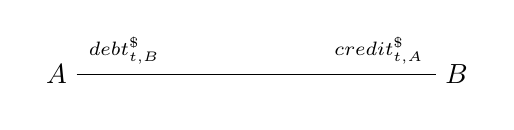
\begin{tikzpicture}
  \matrix [matrix of math nodes,
           column sep={1in,between origins},
           row sep={1in,between origins}]
  {
    |(A)| A &  & |(B)| B \\
  };
  \begin{scope}[every node/.style={midway,auto,font=\scriptsize}]
     \draw  (A)   -- node {$debt^{\$}_{t,B}$ \hspace{0.8in} $credit^{\$}_{t,A}$} (B);
   \end{scope}
\end{tikzpicture}
\caption[A debt-credit relationship between buyer and seller]%
{A debt-credit relationship between the buyer $A$ and seller $B$, which is denominated in the money of account dollar (\$), due at future date of $t$ and worth of \$100 for the good  sold/bought or service rendered. As a result, $A$ has \$100 debt to $B$ and $B$ has \$100 credit on $A$ and the indentity \ref{eq:db_cr_biz} holds. Lastly, $A$ is debtor and $B$ is creditor.}
\label{fig:debt_credit_rel1}
%\vspace{.2in}
\end{figure}

\begin{equation}\label{eq:db_cr_biz}
\left\{
\begin{alignedat}{1}
debt^{\$}_{t,B} \equiv d^{\$}_{t,B} \\
credit^{\$}_{t,A} \equiv c^{\$}_{t,A} \\
\hspace{.1in} d^{\$}_{t,B}=c^{\$}_{t,A}=\$100 \\
\end{alignedat}
\right.
\vspace{.2in}
\end{equation}

In the figure above, the buyer \textit{A} could be either the government or the private indiviual. The seller \textit{B} as private individual could be selling goods she produced or services she had talent in or non-movable property she possessed such land or real-estate. 

It was already mentioned above that the sellers' want of establishing new relationships was driven by the need to acquire credits to liberate themselves from the burden of debt of the previously esablished relationships. There were two groups of counter parties to which private individuals wanted to sell since they were in debt to them: (1)~other private individuals, and (2)~government. While becoming a debtor to the former group was voluntarily, while to be in debt to the latter was enforcable and took place regularly. 

As it was already mentioned the governing authority was the largest and frequent buyer in the community. While mostly buying and having largely nothing for sale, it used levying tax to put private individuals as its debtors, being itself their creditors. As a result, it was creating debt-credit relationships of the type that is shown in Figure \ref{fig:debt_credit_rel2} below.

\begin{figure}[!ht]
\centering
\vspace{.4in}
\captionsetup{width=.9\linewidth,labelfont=bf}
\usetikzlibrary {matrix}
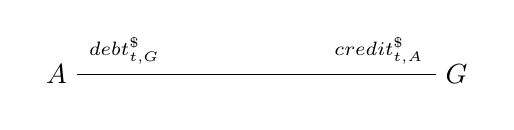
\begin{tikzpicture}
  \matrix [matrix of math nodes,
           column sep={1in,between origins},
           row sep={1in,between origins}]
  {
    |(A)| A &  & |(G)| G \\
  };
  \begin{scope}[every node/.style={midway,auto,font=\scriptsize}]
     \draw  (A)   -- node {$debt^{\$}_{t,G}$ \hspace{0.8in} $credit^{\$}_{t,A}$} (G);
   \end{scope}
\end{tikzpicture}
\caption[A debt-credit relationship between tax-paying individual and government]%
{A debt-credit relationship between the private individual $A$ and government $G$, which is denominated in the money of account dollar (\$), due at future date of $t$ and worth of \$100 tax liability yet to be paid. As a result, $A$ has \$100 debt to $G$ and $G$ has \$100 credit on $A$ and the indentity \ref{eq:db_cr_tax} holds. Lastly, $A$ is debtor and $G$ is creditor.}
\label{fig:debt_credit_rel2}
%\vspace{.2in}
\end{figure}

\begin{equation}\label{eq:db_cr_tax}
\left\{
\begin{alignedat}{1}
debt^{\$}_{t,G} \equiv d^{\$}_{t,G} \\
credit^{\$}_{t,A} \equiv c^{\$}_{t,A} \\
\hspace{.1in} d^{\$}_{t,G}=c^{\$}_{t,A}=\$100 \\
\end{alignedat}
\right.
\vspace{.2in}
\end{equation}

The following quote from \citep{innes1913} provides general logic behind the want among the general public of obtaining credits on the government: 

\begin{quote}
The government by law 
obliges certain selected persons to become its debtors. It declares that
 so-and-so, who imports goods from abroad, shall owe the government so
 much on all that he imports, or that so-and-so, who owns land, shall owe
 to the government so much per acre. This procedure is called levying a
 tax, and the persons thus forced into the position of debtors to the
 government must in theory seek out the holders of the tallies or other
 instrument acknowledging a debt due by the government, and acquire
 from them the tallies by selling to them some commodity or in doing
 them some service, in exchange for which they may be induced to part
 with their tallies. When these are returned to the government treasury,
 the taxes are paid.~\citep[pp.~392-393]{innes1913}
\end{quote}

Being in debt---either due to government or to private individual---enforced an individual, debtor, to seek credits on others via selling her own produce of goods, services, skills or property. This enforcement to act this way came from the \textit{legal} aspect of debt-credit relationship. Here, credit implies the right to \textit{demand and sue}, or go to court, for payment of a debt. Hence, non-payment is not only ``disgraceful", it has real consequences of economic significance and legal character. Non-payment backfires with sanctions of exclusion.

Now, a short summary on payments\index{Payment} can be made. They were made in three ways: (1)~through creation of new \acfp{dcr}, which were denominated in a money of account and these were of the type as shown in Figure \ref{fig:debt_credit_rel1}, p.~\pageref{fig:debt_credit_rel1}, (2)~through re-use or rather assigning of the ``old" (past) debt-credit relationship, which was already existing, to a new creditor in place of the ``old" creditor, and (3)~through destruction or cancellation of the mutual debt-credit relationships between debtor and creditor via the \textit{set-off}\index{Set-off} principle.\index{Set-off!principle of} 

The set-off principle of the third type or way of making a payment is present in the second,too, albeit partially. While the former might be considered as complete or two-sided set-off between counter parties of the \acf{dcr}, the latter is partial or one-sided, where only one side offsets its debt with credit it holds whereas the other side swaps its counter party in the ``old," already existing \ac{dcr}. In the following two subsections these variations of the set-off principle are discussed. The subsection on the complete set-off comes first and to be followed next by the subsection on the partial one. 

\subsubsection*{Payment Method \#2: Complete or Two-Sided Set-off}\index{Set-off!complete or two-sided}

The set-off\index{Set-off!principle of} pricinple in its complete or two-sided form adheres the following criteria. It is said that two \acfp{dcr} qualify for set-off when they are, first, mutual to the counter parties and equal in value; second, they are due in the same time; and, third, they are denominated in the same money of account.\footnote{\citeauthor{innes1913} is not explicit about the third parameter, while discussing the set-off principle.\index{Set-off!principle of} It might be argued that it is not a strict criteria. The counter argument is that in regular every-day payments the set-off principles requires a payer to have credit due today against its debt due today and these must not only equivalent in value, but to be denomianted in the same money of account.} Consider Figure \ref{fig:set-off}, p.~\pageref{fig:set-off}, which illustrates this principle.

There are two counter parties involved and, ordinarily, the principle applies to both as each of them had debt to and credit on the other. Hence, two debt-credit pairs are in play, see section (1) of Figure \ref{fig:set-off}. If debts representing two \acfp{dcr} have different due dates---for example, one is due today and another is due in, say, a month---then set-off does not take place as the debtor whose debt is due in a month has the right to reject the other side's call for payment via set-off.

\begin{figure}[!ht]
\centering
\vspace{.3in}
\captionsetup{width=.8\linewidth,labelfont=bf}
\usetikzlibrary {matrix}
\begin{tikzpicture}
  \draw[help lines,white] (0,0) grid (13,6);
  \node         (A)         at (4,6) {A};
  \node         (B)         at (9,6) {B};
  \node                     at (6.5,5) {(1)};
  \begin{scope}[every node/.style={midway,auto,font=\scriptsize}]
     \draw[black] (A) -- node {$debt^{\$5}_{T,B}$ \hspace{0.8in} $credit^{\$5}_{T,A}$} (B);
     \draw[red]   (4.25,5.9) -- (8.75,5.9) node[sloped,below]  
                          {$credit^{\$5}_{T,B}$ \hspace{.8in} $debt^{\$5}_{T,A}$};
  \end{scope}
  \node         (A)         at (4,3) {A};
  \node         (B)         at (9,3) {B};
  \node                     at (6.5,2) {(2)};
  \begin{scope}[every node/.style={midway,auto,font=\scriptsize}]
     \draw[black] (A) -- node {$debt^{\$5}_{T,B}$ \hspace{0.8in} $credit^{\$5}_{T,A}$} (B);
     \draw[red]   (4.25,2.9) -- (8.75,2.9) node[sloped,below]  
                          {$credit^{\$5}_{T,B}$ \hspace{.8in} $debt^{\$5}_{T,A}$};
     \draw[blue] (4.5,2.5)   -- (5.5,3.5);
     \draw[blue] (4.5,3.5)   -- (5.5,2.5);
     \draw[blue] (7.75,2.5)  -- (8.75,3.5);
     \draw[blue] (7.75,3.5)  -- (8.75,2.5);
  \end{scope}
  \node         (A)         at (4,0) {A};
  \node         (B)         at (9,0) {B};
  \node[gray]               at (6.5,0) {\scriptsize{\textit{no relationships}}};
  \node                     at (6.5,-1) {(3)};
\end{tikzpicture}
\caption[Illustrative example of the set-off principle]%
{Illustrative example of the set-off principle\par\vspace{.05in}(1) Two mutual debt-credit relationships between $A$ and $B$ qualify and ready for set-off as each of them is denominated in the same money of account dollar (\$), has same nominal worh of \$5, and due on the same date that is $T$ days from today.\par (2) Set-off is executed by the debtor $A$ compealing her creditor $B$, see the debt-credit pair in black, to accept $B$'s her own debt now held by $A$, see the debt-credit pair in red, against $B$' credit on $A$; in effect, $A$ releases herself from debt to $B$ by offseting it with credits on $B$ and these are cancelled out for $A$, while $B$ is compealed to do the same with own debts and credits against $A$. For both counter parties these relationships are terminated at the same time.\par(3) There are no debt-credit relationships anymore.}
\label{fig:set-off}
\vspace{.2in}
\end{figure}

\subsubsection*{Payment Method \#3: Partial or One-Sided Set-off}\index{Set-off!partial or one-sided}

The set-off principle in its partial or one-sided form is a more flexible cousin of the complete or two-sided form. Again, there are two counter parties in the existing \acf{dcr}. The difference from the previous case is that these counter parties do not have between them an opposite \ac{dcr} with the same nominal worth, due date, and denomination in the same money of account. However, if the debtor side has another \ac{dcr} it might qualify for a partial set-off and, hence, the payment will take place.

For the purpose of expostion let us agree that existing \ac{dcr} is referred here as primary, while just-mentioned another \ac{dcr} is to be mentioned as secondary. Consider Figure \ref{fig:set-off2} on p.~\pageref{fig:set-off2}, too.

So, the condition for the partial set-off is simple and in the following. If the creditor on the primary \ac{dcr} considers her current position less attractive, preferable or superior to the similar position on the secondary \ac{dcr}, then conditon is met. The partial set-off takes place in the form that debtor in the primary \ac{dcr} offsets its debt with credit she holds within the secondary \ac{dcr}. In other words, this debtor liberates herself from debt by assigning her creditor right within the secondary \ac{dcr} to her now-former creditor.
Also, it might said differently from the side of the creditor within the primary \ac{dcr}, she swapped her credit position within now-terminated primary \ac{dcr} towards a more prefereble creditor position within remaining \ac{dcr}, which was labelled as secondary at the very beginning.

This is a more deatiled description of this way of payment, which might be also called as re-use of existing debt-credit pair.

\begin{figure}[!ht]
\centering
\vspace{.4in}
\captionsetup{width=.8\linewidth,labelfont=bf}
\usetikzlibrary {matrix}
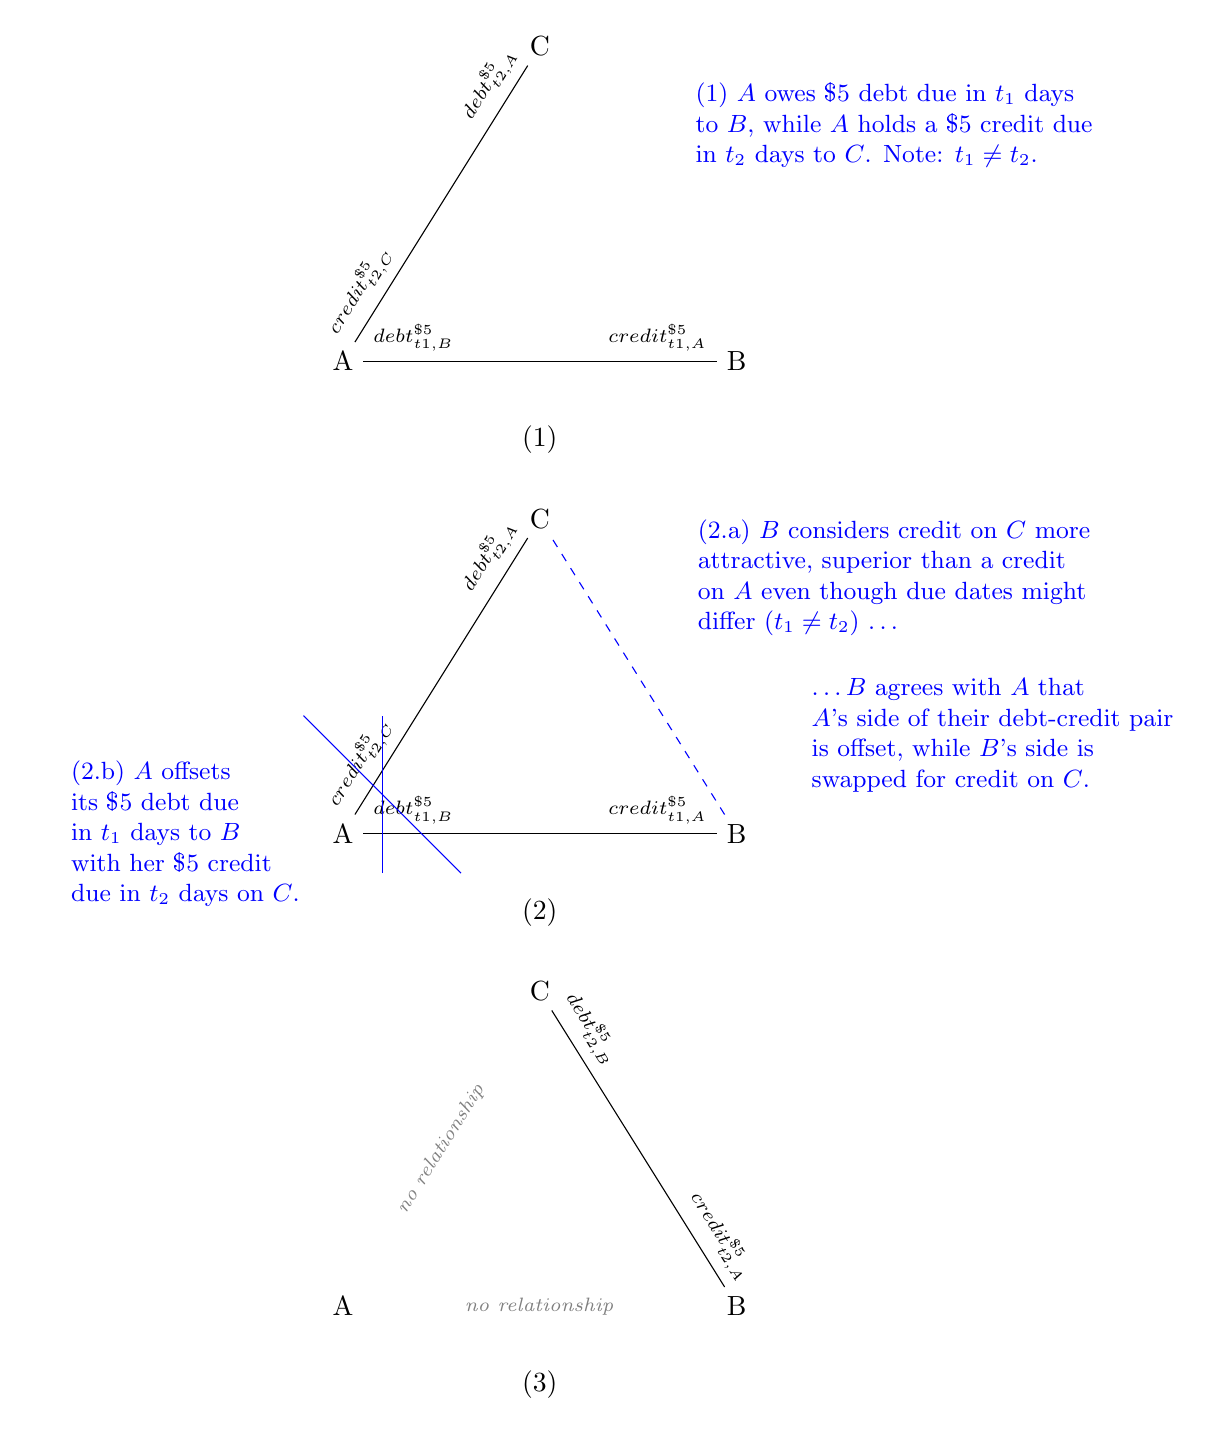
\begin{tikzpicture}
    \draw[help lines,white] (0,0) grid (13,16);
    \node         (A)         at (4,12) {A};
    \node         (B)         at (9,12) {B};
    \node         (C)         at (6.5,16) {C};
    \node                     at (6.5,11) {(1)};
    \begin{scope}[every node/.style={midway,auto,font=\scriptsize}]
        \draw[black] (A) -- (B) node {$debt^{\$5}_{t1,B}$ \hspace{0.7in} $credit^{\$5}_{t1,A}$};
        \draw[black] (A) -- (C) node[sloped,above] {$credit^{\$5}_{t2,C}$ \hspace{0.7in} $debt^{\$5}_{t2,A}$};
    \end{scope}
    \node[blue,align=left,font=\small] at (11,15) {(1) $A$ owes \$5 debt due in $t_1$ days\\to $B$, while $A$ holds a \$5 credit due\\in $t_2$ days to $C$. Note: $t_1 \neq t_2$.};
    \node         (A)         at (4,6) {A};
    \node         (B)         at (9,6) {B};
    \node         (C)         at (6.5,10) {C};
    \node                     at (6.5,5) {(2)};
    \begin{scope}[every node/.style={midway,auto,font=\scriptsize}]
        \draw[black] (A) -- (B) node {$debt^{\$5}_{t1,B}$ \hspace{0.7in} $credit^{\$5}_{t1,A}$};
        \draw[black] (A) -- (C) node[sloped,above] {$credit^{\$5}_{t2,C}$ \hspace{0.7in} $debt^{\$5}_{t2,A}$};
        \draw[blue] (4.5,5.5)   -- (4.5,7.5);
        \draw[blue] (3.5,7.5)   -- (5.5,5.5);
        \draw[blue,dashed] (B) -- (C);
   \end{scope}
   \node[blue,align=left,font=\small] at (11,9.25) {(2.a) $B$ considers credit on $C$ more\\attractive, superior than a credit\\on $A$ even though due dates might\\differ ($t_1 \neq t_2$) \dots};
   \node[blue,align=left,font=\small] at (12.25,7.25) {\dots $B$ agrees with $A$ that\\ $A$'s side of their debt-credit pair\\is offset, while $B$'s side is\\swapped for credit on $C$.};
   \node[blue,align=left,font=\small] at (2,6) {(2.b) $A$ offsets\\its \$5 debt due\\in $t_1$ days to $B$\\with her \$5 credit\\due in $t_2$ days on $C$.};
  \node         (A)         at (4,0) {A};
  \node         (B)         at (9,0) {B};
  \node         (C)         at (6.5,4) {C};
  \node                     at (6.5,-1) {(3)};
  \begin{scope}[every node/.style={midway,auto,font=\scriptsize}]
        \draw[black] (C) -- (B) node[sloped,above] {$debt^{\$5}_{t2,B}$ \hspace{0.7in} $credit^{\$5}_{t2,A}$};
        %\draw[black] (A) -- (C) node[gray,sloped,above] {\textit{no relationships}};
        %\draw[gray,dashed] (A) -- (C);
    \end{scope}
    \node[gray,rotate=0] at (6.5,0) {\scriptsize{\textit{no relationship}}};
    \node[gray,rotate=58] at (5.25,2) {\scriptsize{\textit{no relationship}}};
\end{tikzpicture}
\caption[Illustrative example of the partial or one sided set-off]%
{Illustrative example of the partial or one sided set-off.}
\label{fig:set-off2}
\vspace{.3in}
\end{figure}

\subsubsection*{Interplay of Three Methods of Payment}

From early on in the evolution of payment, debt-credit relationships had been dated and followed the set-off\index{Set-off} principle: ``[d]ebts and credits to be set off against each other must be `due` at the \textit{same} time"\index{Set-off!principle of}~\citep[p.~404, emphasis added]{innes1913}. In terms of time sequence, a set-off requires two pre-existing \acfp{dcr}. And it just underscores the dynamic significance of payments: some debt-credit pairs are created anew as payment, some pairs are ``old" or already existing and used as payments since new creditors displace the ``old" one, and lastly payments via the set-off principle cancel out pre-existing debt-credit pairs.      

\begin{quote}
Whatever commercial or financial transaction we examine, whether it
 be the purchase of a penn'orth of vegetables in the market or the issue of a 
billion dollar loan by a government, we find in each and all of them the
 same principle involved; \textit{either an old credit is transferred or new ones are 
created}, and a State or a banker or a peasant is prosperous or bankrupt
 according as the principle is observed or not, that debts, as they fall due,
 must be met by credits available, at the same moment. \dots  It must be
 remembered that a credit due for payment at a future time cannot be set
 off against a debt due to another banker immediately. Debts and credits
 to be set off against each other must be 'due' at the same time.~\citep[p.~404, emphasis added]{innes1913}
\end{quote}

Consider a hypothetical example that builds upon Figure~\ref{fig:debt_credit_rel1} on p.~\pageref{fig:debt_credit_rel1}. That chart depicted a transaction that took place on date \(t=0\) and established the following debt-credit relationship: private individual \textit{A} bought goods worth of \$100 from another private individual \textit{B} by providing the latter with his acknowledgement of debt, which was due in 90 days (\(t=90\)) or three months from the date of transaction. Then, over the course of remaining time before the due date, person \textit{A} had to find buyers for the goods/services she has for sale. Recall that by selling she could accumulate credits on other private individuals. Within that period of 90 days, the most important factor to \textit{A} was to find such a buyer or buyers, who had at least \$100 credits on person \textit{B} and these credits, \textit{B}'s acknowledgements of debt, themselves were due on the \textit{same} date as the above-mentioned acknowledgement of debt by \textit{A}. It is assumed that person \textit{C} had such credits thanks to previosuly selling goods of own produce to \textit{B}. Then, \textit{C}, while buying from person \textit{A}, handed over credits on person \textit{B} to the seller \textit{A}. As a result, \textit{A} obtained \$100 credit on \textit{B} and \$100 debt to \textit{B}. In other words, \textit{A} had two debt-credit relationships with \textit{B} of same worth and due date, which were opposite in term of debt and credit. The same was true for \textit{B}: she hold \$100 credit on \textit{A} from the very beginning, but then her \$100 debt became owed to \textit{A}. Two mutual debt-credit relationships between \textit{A} and \textit{B} are ready for a set-off, mutual cancellation of indebtedness. Thus, on the 90th day from the very first transaction, when \textit{A}'s \$100 debt to \textit{B} was due, she liberated herself from debt by delivering to \textit{B} the latter's acknowledgement of debt that had same worth and due on the same day. According to the basic priciples of debt-credit relationships honored widely, \textit{B} could not refuse and accepted in payment her own debt against credit she had on \textit{A}. The set-off\index{Set-off} principle worked for both counter parties \textit{A} and  \textit{B}. See Figure \ref{fig:debt_credit_rel3} on p.~\pageref{fig:debt_credit_rel3}.

In this example all three methods have been in the display. Initially, the payment created a debt-credit pair between \textit{A} and \textit{B}. Then, the payment between \textit{A} and \textit{C} took the form of assigning \textit{A} as creditor instead of \textit{C} to the already exisiting debt-credit pair, in which \textit{B} was the debtor. Lastly, the payment took the form of set-off at the very end of the exposition. 

\begin{figure}[ht]%[!ht]
\centering
\vspace{.4in}
\captionsetup{width=1\linewidth,labelfont=bf}
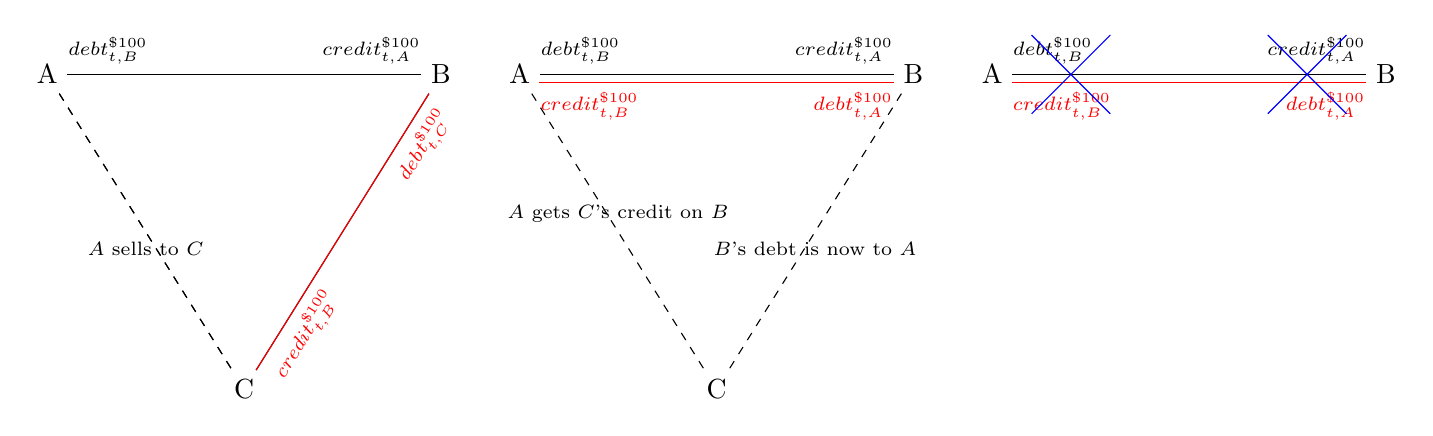
\begin{tikzpicture}
  \draw[help lines,white] (0,0) grid (17,4);
  \node         (A)         at (0  ,4) {A};
  \node         (B)         at (5  ,4) {B};
  \node         (C)         at (2.5,0) {C};
  \draw         (A)         to (B);
  \draw         (B)         to (C);
  \draw[dashed] (A)         to (C);
  \node         (D)         at (6  ,4) {A};
  \node         (E)         at (11 ,4) {B};
  \node         (F)         at (8.5,0) {C};
  \node         (G)         at (12 ,4) {A};
  \node         (H)         at (17 ,4) {B};
  \begin{scope}[every node/.style={midway,auto,font=\scriptsize}]
     \draw[black] (A)   -- node {$debt^{\$100}_{t,B}$ \hspace{.8in} $credit^{\$100}_{t,A}$} (B);
     \draw[red]   (C)   -- node [sloped,below] 
                          {$credit^{\$100}_{t,B}$ \hspace{.6in} $debt^{\$100}_{t,C}$} (B);
     \draw[dashed] (A)   -- node [below] {$A$ sells to $C$} (C);
     \draw[black] (D)   -- node {$debt^{\$100}_{t,B}$ \hspace{.8in} $credit^{\$100}_{t,A}$} (E);
     \draw[red]   (6.25,3.9) -- (10.75,3.9) node[midway,below]  
                          {$credit^{\$100}_{t,B}$ \hspace{.8in} $debt^{\$100}_{t,A}$};
     \draw[dashed] (D)   -- node [above] {$A$ gets $C$'s credit on $B$} (F);
     \draw[dashed] (E)   -- node [below] {$B$'s debt is now to $A$} (F);
     \draw[black] (G)   -- node {$debt^{\$100}_{t,B}$ \hspace{.8in} $credit^{\$100}_{t,A}$} (H);
     \draw[red]   (12.25,3.9) -- (16.75,3.9) node[midway,below]  
                          {$credit^{\$100}_{t,B}$ \hspace{.8in} $debt^{\$100}_{t,A}$};
   \end{scope}
   \draw[blue] (12.5,3.5) -- (13.5,4.5);
   \draw[blue] (12.5,4.5) -- (13.5,3.5);
   \draw[blue] (15.5,4.5) -- (16.5,3.5);
   \draw[blue] (15.5,3.5) -- (16.5,4.5);
\end{tikzpicture}
\caption[Debt-credit relationships while paying on private debt]%
{A set of debt-credit relationships that allow $A$, the debtor to $B$, to pay on date $t$: (1) $A$ seeks credits on $B$ that due on date $t$, too, by selling goods to $C$, who had sold goods to $B$ previously; (2) $C$ transfers his credits on $B$ for $A$ in exchange of goods sold and now $B$'s debt to $C$ transfered, too, towards $A$; (3) lastly, $A$ offsets his debt to $B$ with credit on $B$ and the latter accepts the same for own credit and debt to $A$ -- both sides' mutual debts and credits are extinct.}
\label{fig:debt_credit_rel3}
\vspace{.2in}
\end{figure}

\begin{figure}[ht]%[!ht]
\centering
\vspace{.4in}
\captionsetup{width=1\linewidth,labelfont=bf}
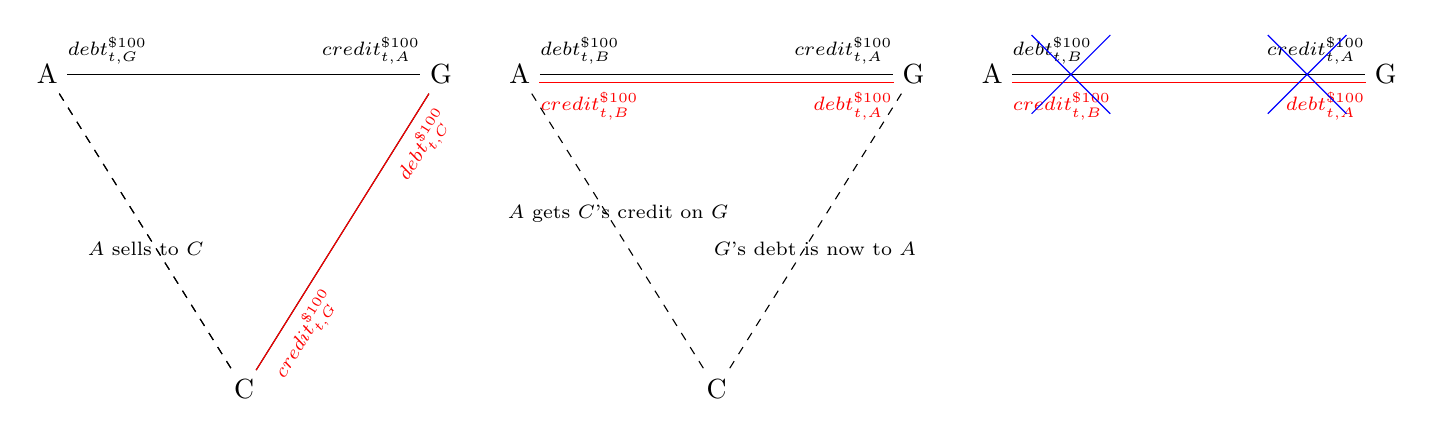
\begin{tikzpicture}
  \draw[help lines,white] (0,0) grid (17,4);
  \node         (A)         at (0  ,4) {A};
  \node         (B)         at (5  ,4) {G};
  \node         (C)         at (2.5,0) {C};
  \draw         (A)         to (B);
  \draw         (B)         to (C);
  \draw[dashed] (A)         to (C);
  \node         (D)         at (6  ,4) {A};
  \node         (E)         at (11 ,4) {G};
  \node         (F)         at (8.5,0) {C};
  \node         (G)         at (12 ,4) {A};
  \node         (H)         at (17 ,4) {G};
  \begin{scope}[every node/.style={midway,auto,font=\scriptsize}]
     \draw[black] (A)   -- node {$debt^{\$100}_{t,G}$ \hspace{.8in} $credit^{\$100}_{t,A}$} (B);
     \draw[red]   (C)   -- node [sloped,below] 
                          {$credit^{\$100}_{t,G}$ \hspace{.6in} $debt^{\$100}_{t,C}$} (B);
     \draw[dashed] (A)   -- node [below] {$A$ sells to $C$} (C);
     \draw[black] (D)   -- node {$debt^{\$100}_{t,B}$ \hspace{.8in} $credit^{\$100}_{t,A}$} (E);
     \draw[red]   (6.25,3.9) -- (10.75,3.9) node[midway,below]  
                          {$credit^{\$100}_{t,B}$ \hspace{.8in} $debt^{\$100}_{t,A}$};
     \draw[dashed] (D)   -- node [above] {$A$ gets $C$'s credit on $G$} (F);
     \draw[dashed] (E)   -- node [below] {$G$'s debt is now to $A$} (F);
     \draw[black] (G)   -- node {$debt^{\$100}_{t,B}$ \hspace{.8in} $credit^{\$100}_{t,A}$} (H);
     \draw[red]   (12.25,3.9) -- (16.75,3.9) node[midway,below]  
                          {$credit^{\$100}_{t,B}$ \hspace{.8in} $debt^{\$100}_{t,A}$};
   \end{scope}
   \draw[blue] (12.5,3.5) -- (13.5,4.5);
   \draw[blue] (12.5,4.5) -- (13.5,3.5);
   \draw[blue] (15.5,4.5) -- (16.5,3.5);
   \draw[blue] (15.5,3.5) -- (16.5,4.5);
\end{tikzpicture}
\caption[Debt-credit relationships while paying on tax debt]%
{A set of debt-credit relationships that allow $A$, the taxpayer, to redeem himself with the government on date $t$: (1) $A$ seeks credits on government $G$ that due on date $t$, too, by selling goods to $C$, who had sold goods or services to $G$ previously; (2) $C$ transfers his credits on $G$ for $A$ in exchange of goods sold and now $G$'s debt to $C$ transfered, too, towards $A$; (3) lastly, $A$ offsets his debt to $G$ with credit on $G$ and the latter does the same for own credit and debt to $A$ -- both sides' mutual debts and credits are extinct, i.e. taxes are paid.}
\label{fig:debt_credit_rel4}
\vspace{.2in}
\end{figure}

Another hypothetical example builds upon the debt-credit relationship first depicted in Figure~\ref{fig:debt_credit_rel2} on p.~\pageref{fig:debt_credit_rel2}. It depicted the following debt-credit relationship: the government \textit{G} levied a tax worth of \$100 on the private individual \textit{A}, which was due in 90 days or three months (\(t=90\)). Hence, \textit{G} became creditor of \textit{A}, while \textit{A} became debtor to \textit{G}. Within the remaining 90 day period, \textit{A} had to find credits on government of \textit{same} worth and due date. She could sell her skills and talents to the government or sell her own produce to other private individuals, who previously were working for and selling to government themselves and hence possessed acknowledgements of debt by the government. It is assumed that person \textit{C} was such a person with required credits on government. Then, similarly to the previous example, \textit{C} bought goods from \textit{A} by handing over the acknowledgements of debt by the government. As a result, private individual \textit{A} had two debt-credit relationships with govermennt of \$100 worth and have same due date, which were opposite in term of debt and credit. Similarly, government \textit{G} had two relationships with respect to \textit{A}. Then, on the due date that is on 90th day since the original relationship was established between \textit{G} and \textit{A}, the latter handed over to the government its, \textit{G}'s, acknowledgements of debt. Such an act was as an invitation to set-off\index{Set-off} mutual indebtedness that \textit{G} not only could not refuse more than that it was an original idea of social organization through debt-credit relationships. See Figure~\ref{fig:debt_credit_rel4} on p.~\pageref{fig:debt_credit_rel4}.

In this example, however, the payments were of two types only: as re-use of the existing debt-credit pair and then as set-off\index{Set-off} of the mutual pairs. This is because the debt-credit pair between \textit{A} and \textit{G} was produced by the latter lavying tax. This said, however, at the backgound there is a prior debt-credit pair between \textit{G} and \textit{C} that was created anew as the former was buying some good or service from the latter by paying with acknowledgement of debt due on the future date of \textit{t}.

As commerce widened the debt-credit relationships had become more complicated as shown on Figure~\ref{fig:six_merchants_trade1} on p.~\pageref{fig:six_merchants_trade1} below. These examples are replicated from \citep[pp.~402-403]{innes1913}.

\begin{figure}[!ht]
\vspace{0.4in}
\centering
\captionsetup{width=1\linewidth,labelfont=bf}
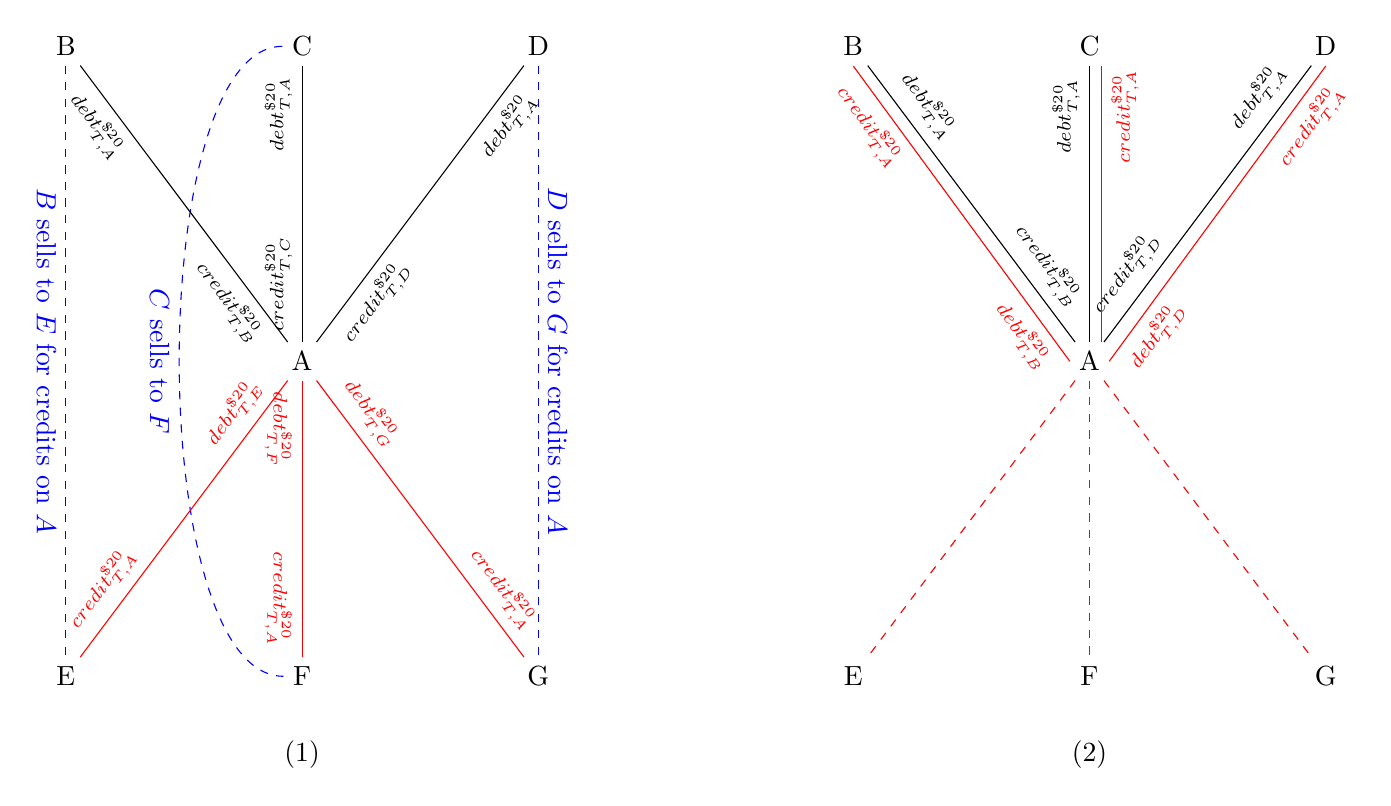
\begin{tikzpicture}
  \draw[help lines,white] (0,0) grid (16,8);
  \node         (A)         at (3,4) {A};
  \node         (B)         at (0,8) {B};
  \node         (C)         at (3,8) {C};
  \node         (D)         at (6,8) {D};
  \node         (E)         at (0,0) {E};
  \node         (F)         at (3,0) {F};
  \node         (G)         at (6,0) {G};
  \node                     at (3,-1) {(1)};
  \draw[dashed,blue] (B) -- node[below,sloped] {$B$ sells to $E$ for credits on $A$} (E);
  \draw[dashed,blue] (C) .. controls +(left:2cm) and +(left:2cm) .. 
                       node[below,sloped] {$C$ sells to $F$} (F);
  \draw[dashed,blue] (D) -- node[above,sloped] {$D$ sells to $G$ for credits on $A$} (G);
  \begin{scope}[every node/.style={midway,auto,font=\scriptsize}]
     \draw[black] (A)   -- node [sloped,below] 
                {$debt^{\$20}_{T,A}$ \hspace{.6in} $credit^{\$20}_{T,B}$} (B);
     \draw[black] (A)   -- node [sloped,above] 
                {$credit^{\$20}_{T,C}$ \hspace{.35in} $debt^{\$20}_{T,A}$} (C);
     \draw[black] (A)   -- node [sloped,below] 
                {$credit^{\$20}_{T,D}$ \hspace{.6in} $debt^{\$20}_{T,A}$} (D);
     \draw[red] (A)   -- node [sloped,above] 
                {$credit^{\$20}_{T,A}$ \hspace{.6in} $debt^{\$20}_{T,E}$} (E);
     \draw[red] (A)   -- node [sloped,below] 
                {$debt^{\$20}_{T,F}$ \hspace{.35in} $credit^{\$20}_{T,A}$} (F);
     \draw[red] (A)   -- node [sloped,above] 
                {$debt^{\$20}_{T,G}$ \hspace{.6in} $credit^{\$20}_{T,A}$} (G);
  \end{scope}
  \node         (A1)         at (13,4) {A};
  \node         (B1)         at (10,8) {B};
  \node         (C1)         at (13,8) {C};
  \node         (D1)         at (16,8) {D};
  \node         (E1)         at (10,0) {E};
  \node         (F1)         at (13,0) {F};
  \node         (G1)         at (16,0) {G};
  \node                     at (13,-1) {(2)};
  \draw[dashed,red] (A1) to (E1);
  \draw[dashed,red] (A1) to (F1);
  \draw[dashed,red] (A1) to (G1);
    \begin{scope}[every node/.style={midway,auto,font=\scriptsize}]
     \draw[black] (A1)   -- node [sloped,above] 
                {$debt^{\$20}_{T,A}$ \hspace{.5in} $credit^{\$20}_{T,B}$} (B1);
     \draw[black] (A1)   -- node [sloped,above] 
                {$\space\space$ \hspace{.8in} $debt^{\$20}_{T,A}$} (C1);
     \draw[black] (A1)   -- node [sloped,above] 
                {$credit^{\$20}_{T,D}$ \hspace{.6in} $debt^{\$20}_{T,A}$} (D1);
     \draw[red] (12.75,4) -- (10,7.75) node[sloped,below]  
                          {$credit^{\$20}_{T,A}$ \hspace{.8in} $debt^{\$20}_{T,B}$};
     \draw[red] (13.15,4.25) -- (13.15,7.75) node[sloped,below]  
                          {$\space\space$ \hspace{.8in} $credit^{\$20}_{T,A}$};
     \draw[red] (13.25,4) -- (16,7.75) node[sloped,below]  
                          {$debt^{\$20}_{T,D}$ \hspace{.8in} $credit^{\$20}_{T,A}$};
  \end{scope}
\end{tikzpicture}
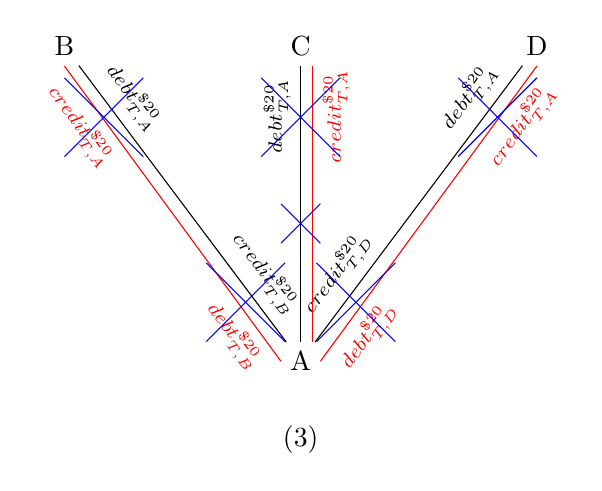
\begin{tikzpicture}
  \draw[help lines,white] (0,0) grid (6,4);
  \node         (A)         at (3,0) {A};
  \node         (B)         at (0,4) {B};
  \node         (C)         at (3,4) {C};
  \node         (D)         at (6,4) {D};
  \node                     at (3,-1) {(3)};
  \begin{scope}[every node/.style={midway,auto,font=\scriptsize}]
     \draw[black] (A)   -- node [sloped,above] 
                {$debt^{\$20}_{T,A}$ \hspace{.6in} $credit^{\$20}_{T,B}$} (B);
     \draw[black] (A)   -- node [sloped,above] 
                {$\space\space$ \hspace{.8in} $debt^{\$20}_{T,A}$} (C);
     \draw[black] (A)   -- node [sloped,above] 
                {$credit^{\$20}_{T,D}$ \hspace{.6in} $debt^{\$20}_{T,A}$} (D);
     \draw[red] (2.75,0) -- (0,3.75) node[sloped,below]  
                          {$credit^{\$20}_{T,A}$ \hspace{.8in} $debt^{\$20}_{T,B}$};
     \draw[red] (3.15,0.25) -- (3.15,3.75) node[sloped,below]  
                          {$\space\space$ \hspace{.8in} $credit^{\$20}_{T,A}$};
     \draw[red] (3.25,0) -- (6,3.75) node[sloped,below]  
                          {$debt^{\$20}_{T,D}$ \hspace{.8in} $credit^{\$20}_{T,A}$};
  \end{scope}
  \draw[blue] (0,2.6)    -- (1,3.6);
  \draw[blue] (0,3.6)    -- (1,2.6);
  \draw[blue] (2.5,2.6)  -- (3.5,3.6);
  \draw[blue] (2.5,3.6)  -- (3.5,2.6);
  \draw[blue] (5,2.6)    -- (6,3.6);
  \draw[blue] (5,3.6)    -- (6,2.6);
  \draw[blue] (1.8,0.25) -- (2.8,1.25);
  \draw[blue] (1.8,1.25) -- (2.8,0.25);
  \draw[blue] (3.2,0.25) -- (4.2,1.25);
  \draw[blue] (3.2,1.25) -- (4.2,0.25);
  \draw[blue] (2.75,1.5) -- (3.25,2);
  \draw[blue] (2.75,2)   -- (3.25,1.5);
\end{tikzpicture}
\caption[Debt-credit relationships, when $A$ was buying and selling with $B,C,D,E,F,G$]%
{Debt-credit relationships, when $A$ was buying and selling with $B,C,D,E,F,G$.\par\vspace{0.05in}(1): $A$ sells goods to $B$, $C$ and $D$ by accepting their acknowledgments of debt. Also, $A$ buys goods from $E$, $F$ and $G$ and gives his acknowledgment of debt to each in payment. Then, $B$, $C$ and $D$ sell goods to $E$, $F$ and $G$ and take in payment the acknowledgements of debt given by $A$.\par (2): Now, $B$, $C$ and $D$ have debts and credits with respect to $A$ so that they could then present these credits to $A$ and by so doing release themselves from their debt.\par (3): $B$, $C$ and $D$ present to $A$ credits on him and $A$ accepts his own debts to cancel $A$'s credits on $B$, $C$ and $D$. Mutual debts and credits are cancelled, extinct.}
\label{fig:six_merchants_trade1}
\vspace{.2in}
\end{figure}

As activities of commerce and governing authority were taking place, individuals accumulate certain amount of credits and debts, all of which had different due dates and, theoretically, could be denominated in different money of accounts (however, as of now, the exposition is limited to a single money of account). The concept solvency was recognized in the following terms:

\begin{quote}
Debts due at a certain noment can only be cancelled by being offset
 against credits which become available at that moment; that is to say
 that a creditor cannot be compelled to accept in payment of a debt due
 to him an acknowledgment of indebtedness which he himself has given
 and which only falls due at a later time. Hence it follows that a man is
 \textit{only solvent} if he has immediately available credits at least equal to the
 amount of his debts immediately due and presented for payment. If therefore, the sum of his immediate debts exceeds the sum of his immediate credits, the real value of these debts to his creditors will fall to an amount which will make them equal to the amount of his credits. This
 is one of the most important principles of commerce.~\citep[pp.~393-394, emphasis added]{innes1913}
\end{quote}

Then, from the above description derives the following depiction of an hypothetical individual's collection of debts and credits. This is done via the concept of the balance sheet, see Figure \ref{fig:bs1} below. This balance sheet describes only relational positions of an individual with respect to the counter parties, it implies that non-relational positions such as owned tangable property is not shown there yet. And unlike the traditional presentation of the balance sheet, which has sums of assets in strict equivalence to sum of liabilities and equity, the one at Figure \ref{fig:bs1} implies that sum of credits is not nessesarily equal to sum of debts. This is because, with matters of relational debts and credits, there is a concept of solvency of an individual. The solvency criteria is presented by Equation~\ref{eq:solv_rule} below.
 
\begin{figure}[!ht]
\hspace{.3in}
\captionsetup{width=.8\linewidth,labelfont=bf}
  \centering
  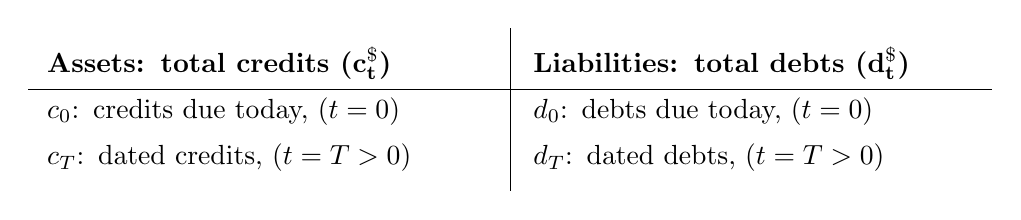
\begin{tikzpicture}
    \matrix (m) [matrix of nodes,
             nodes = {text width=2.2in, minimum height=.2in, align=left},
             column sep=1em,
             row 1/.style={align=center, font=\bfseries},
            ]
      {
      Assets: total credits ($\mathbf{c^{\$}_t}$) & Liabilities: total debts ($\mathbf{d^{\$}_t}$) \\
      $c_0$: credits due today, ($t=0$)     & $d_0$: debts due today, ($t=0$) \\
      $c_{\tiny T}$: dated credits, ($t=T>0$) & $d_{\tiny T}$: dated debts, ($t=T>0$) \\
      };
      \draw[thin]  (m-1-2.south -| m.west) -- (m-1-2.south -| m.east)
                        (m.north) -- (m.south);              
  \end{tikzpicture}
  \caption[A balance sheet of an individual $A$ as collection of debts and credits]%
  {Balance sheet of an individual person, merchant or of a business entity $A$ with outstanding debts and credits that are denominated in a single money-of-account such as (\$) dollar and in terms of their maturity $t=0,1,2,...$, where $t=0$ is due today, $t=1$ is due in 1 day from now/today, and so on.}
  \label{fig:bs1}
\end{figure}

\begin{equation}\label{eq:solv_rule}
\begin{split}
    & d_0=f(c_0)= 
    \begin{dcases}
    d_0=d^{\ddag}_t & \text{holding par, if } c_0 \geq d_0 \\
    d_0=c_0<d^{\ddag}_t & \text{revalued below par, if } c_0 < d_0 \\
    \end{dcases} \\
    & \text{where } d^{\ddag}_t \text{ is value of debt-credit pairs at, \textit{t}, time of creation} 
\end{split}
\end{equation}

The above-mentioned figure and equation should not be considered as a static matter. Instead, it is an explicitly dynamic one as time goes by and debts from dated \acfp{dcr} eventually approach the due date---\textit{t} runs to zero, \(t=0\)---every next day, or continuously. Hence, today's due debts (\(d_0\)) must be offset by the credits due today (\(c_0\)). And this off-set rule must be maintained every single day, when past debts arrive at the payment date. In order to avoid violation of the solvency Equation \ref{eq:solv_rule} an individual must sell goods/services to others and obtaining credits on other members of the community/society.

The two examples above might appear quite cumbersome from the modern-day point of view. The evolutionary element makes them that different from what is so customary today. Back then, these relationships were dated, in other words their due dates extended well into the future. In effect, the payment via off-set was expected in several months, not days. Thanks to that the payments via set-off were taking place at the special events or gatherings fairs, where the main activity was debtors and creditors meeting up and setting off mutual debts and credits. Periodical fairs served as clearing houses of commerce and those debt-credit pairs just mentioned:\index{Clearing house!fairs}

\begin{quote}
The clearing houses of old were the great periodical fairs, whither went 
merchants great and small, bringing with them their tallies, to settle their
mutual debts and credits. \dots The greatest of these fairs
in England was that of St. Giles in Winchester, while the most famous
probably in all Europe were those of Champagne and Brie in France, to
which came merchants and bankers from all countries. Exchange booths
were established and debts and credits were cleared to enormous
amounts without the use of a single coin. \dots  Nor was the custom of holding fairs confined to mediaeval Europe. They were held in ancient Greece under the name of \textit{panegyris}
and in Rome they were called \textit{nundinae}, a name which in the middle ages
was also frequently used. They are known to have been held in
Mesopotamia and in India. In Mexico they are recorded by the historians
of the conquest, and not many years ago at the fairs of Egypt, customs
might have been seen which were known to Herodotus.~\citep[pp.~398-399, emphasis original]{innes1913}
\end{quote}

In parralel with commercial fairs, the governing authority ran its own clearing activities by setting off debts and credits where it was a side of the repsective pairs. The English practice was:

\begin{quote}
Practically the entire business of the English Exchequer consisted in the issuing and receiving of tallies, \dots, in keeping the accounts of the government debtors and creditors, and in cancelling the tallies when returned to the Exchequer. It was, in fact, the great clearing house for government credits and debts.~\citep[p.~398]{innes1913}
\end{quote}

The above-mentioned fairs were a social technology or devices of wholesale cancellation of mutual debts and credits in a dynamic chain of events. By itself such cancellation confirmed one's solvency, or ability to make payment through set-off\index{Set-off}, and hence that individual and others like her were opening up for creation of new \acfp{dcr} in the period between the fairs. The latter, the newly created debt-credit pairs, then would be subject for cancellation at a fair taking place next time. These dynamic chains were spread over historical time. 

New technologies and innovations were coming to narrow down that time lag between creation and then confirmaion of the solvency via the set-off payment. 

\subsubsection{Evolution of Clearing Houses}\label{sec:evolution}

Over time, on the back of evolution in payments the governments paved the way for banks taking over as clearing houses for debts and credits instead of fairs.\index{Clearing house!by banker} The very early mass communication technology was postal service recognized and organized by the governing authority.\footnote{Even later, the national postal services became a backbone of the most effective international cooperation embodied the International Postal Union, which operated ``long before 1900" \citep[p.~2]{beyen1949}.}

\begin{quote}
Little by little as governments developed their postal systems and powerful banking corporations grew up, the value of fairs as clearing houses dwindled, and they ceased to be frequented for that purpose, long remaining as nothing but festive gatherings until at last there linger but few, and those a mere shadow of their golden greatness.~\citep[p.~397]{innes1913} \par
\dots as soon as commerce widened out, and the various debtors and creditors lived far apart and  were unacquainted with one another, it is obvious that without some system of centralizing debts and credits commerce would not go on. Then arose the merchant or banker, the latter being merely a more specialized variety of the former.~\citep[p.~403]{innes1913}
\end{quote}
 
Bankers developed two methods of dealing with debts and credits: (1)~by discounting bills, see Figure \ref{fig:bank_clearing_house1}, on p.~\pageref{fig:bank_clearing_house1} below; and (2)~by making loans, see Figure \ref{fig:bank_clearing_house2} on p.~\pageref{fig:bank_clearing_house2} below. These figures replicate the examples of banks' centralization of debt-credit pairs on themselves given in \citep[pp.~402-403]{innes1913}. 

The discounting bills by banks aims at the already established debt-credit relations between individuals such as shown in Figure \ref{fig:bank_clearing_house1}. There are seven individuals \textit{A, B, C, D, E, F, G} in this example, of which \textit{A} is the most active since she sold to \textit{B, C, D} some goods and services and bought from \textit{E, F, G}. On the back of these transactions, which by assumption all had same value and same due date, \textit{A} has credits on \textit{B, C, D} and debts to \textit{E, F, G}. What banker \textit{R} does is buying credits held by \textit{A} on \textit{B, C, D}, turning herselve into a debtor to \textit{A} while becoming a creditor to \textit{B, C, D}. In similar way, the banker \textit{R} buys credits held by \textit{E, F, G} on \textit{A}, becoming debtor to  \textit{E, F, G} and creditor to \textit{A}. This is shown in sections (1) and (2) of Figure \ref{fig:bank_clearing_house1}. Note, too, that there are two mutual and opposite debt-credit pairs between banker \textit{R} and individual \textit{A}. When due date arrives on these pairs, both of these counter parties use the set-off principle by matching debts with credits and their relationships are termintaed, or cancelled out. Their names drop out from the books they keep for accounting their overall debts and credits. This is depicted in section (3) of Figure \ref{fig:bank_clearing_house1}.

\begin{figure}[!ht]
\vspace{0in}
\centering
\captionsetup{width=1\linewidth,labelfont=bf}
% Top part of the Figure
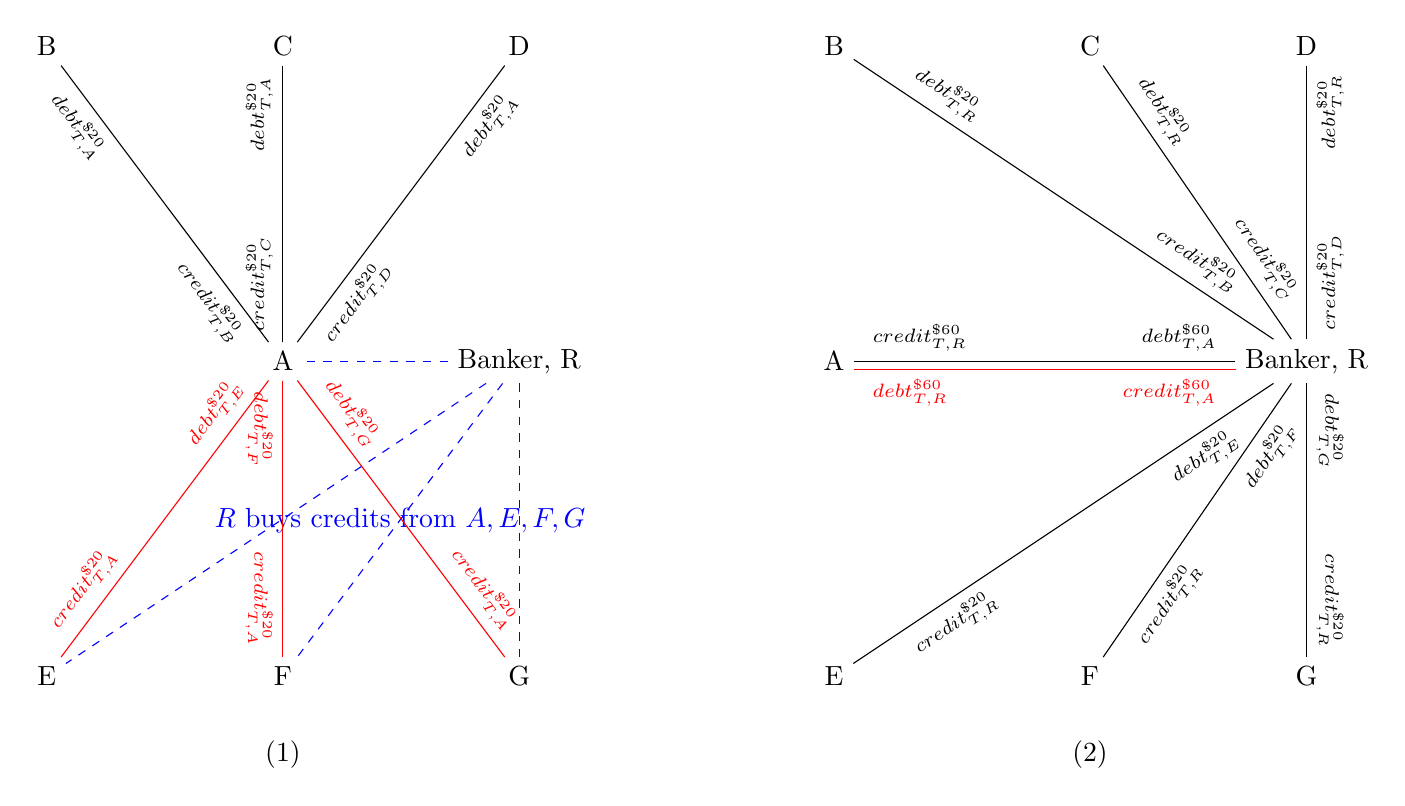
\begin{tikzpicture}
  \draw[help lines,white] (0,0) grid (16,8);
  \node         (A)         at (3,4) {A}; % at (3,4) {A};
  \node         (B)         at (0,8) {B};
  \node         (C)         at (3,8) {C};
  \node         (D)         at (6,8) {D};
  \node         (E)         at (0,0) {E};
  \node         (F)         at (3,0) {F};
  \node         (G)         at (6,0) {G};
  \node         (b)         at (6,4) {Banker, R};
  \draw[dashed,blue] (b) -- (A);
  \draw[dashed,blue] (b) -- (E);
  \draw[dashed,blue] (b) -- node[midway] {$R$ buys credits from $A,E,F,G$} (F);
  \draw[dashed,blue] (b) -- (G);
  \begin{scope}[every node/.style={midway,auto,font=\scriptsize}]
     \draw[black] (A)   -- node [sloped,below] 
                {$debt^{\$20}_{T,A}$ \hspace{.6in} $credit^{\$20}_{T,B}$} (B);
     \draw[black] (A)   -- node [sloped,above] 
                {$credit^{\$20}_{T,C}$ \hspace{.35in} $debt^{\$20}_{T,A}$} (C);
     \draw[black] (A)   -- node [sloped,below] 
                {$credit^{\$20}_{T,D}$ \hspace{.6in} $debt^{\$20}_{T,A}$} (D);
     \draw[red] (A)   -- node [sloped,above] 
                {$credit^{\$20}_{T,A}$ \hspace{.6in} $debt^{\$20}_{T,E}$} (E);
     \draw[red] (A)   -- node [sloped,below] 
                {$debt^{\$20}_{T,F}$ \hspace{.35in} $credit^{\$20}_{T,A}$} (F);
     \draw[red] (A)   -- node [sloped,above] 
                {$debt^{\$20}_{T,G}$ \hspace{.6in} $credit^{\$20}_{T,A}$} (G);
  \end{scope}
  \node         (A1)         at (10,4) {A};
  \node         (B1)         at (10,8) {B};
  \node         (C1)         at (13.25,8) {C};
  \node         (D1)         at (16,8) {D};
  \node         (E1)         at (10,0) {E};
  \node         (F1)         at (13.25,0) {F};
  \node         (G1)         at (16,0) {G};
  \node         (b1)         at (16,4) {Banker, R};
    \begin{scope}[every node/.style={midway,auto,font=\scriptsize}]
     \draw[black] (A1)   -- node [sloped,above] 
                {$credit^{\$60}_{T,R}$ \hspace{.8in} $debt^{\$60}_{T,A}$} (b1);
     \draw[black] (b1)   -- node [sloped,above] 
                {$debt^{\$20}_{T,R}$ \hspace{1.0in} $credit^{\$20}_{T,B}$} (B1);
     \draw[black] (b1)   -- node [sloped,above] 
                {$debt^{\$20}_{T,R}$ \hspace{.4in} $credit^{\$20}_{T,C}$} (C1);
     \draw[black] (b1)   -- node [sloped,below] 
                {$credit^{\$20}_{T,D}$ \hspace{.35in} $debt^{\$20}_{T,R}$} (D1);
     \draw[black] (b1)   -- node [sloped,below] 
                {$credit^{\$20}_{T,R}$ \hspace{1in} $debt^{\$20}_{T,E}$} (E1);
     \draw[black] (b1)   -- node [sloped,below] 
                {$credit^{\$20}_{T,R}$ \hspace{.4in} $debt^{\$20}_{T,F}$} (F1);
     \draw[black] (b1)   -- node [sloped,above] 
                {$debt^{\$20}_{T,G}$ \hspace{.35in} $credit^{\$20}_{T,R}$} (G1);
     \draw[red] (10.25,3.9) -- (15.1,3.9) node[sloped,below]  
                          {$debt^{\$60}_{T,R}$ \hspace{.8in} $credit^{\$60}_{T,A}$};
  \end{scope}
  \node at (3,-1) {(1)};
  \node at (13.25,-1) {(2)};
\end{tikzpicture}
% Bottom part of the Figure
\vspace{0in}
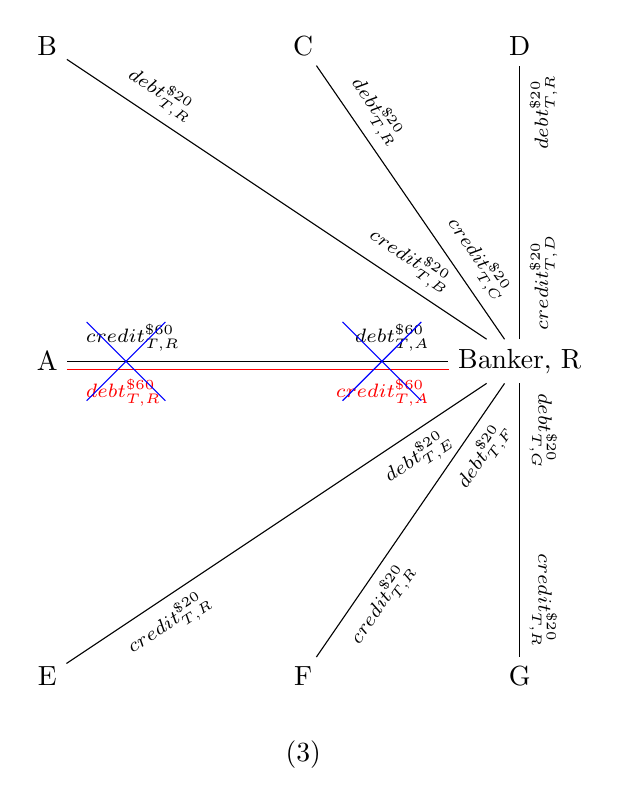
\begin{tikzpicture}
  \draw[help lines,white] (0,0) grid (6,8);
  \node         (A1)         at (0,4) {A};
  \node         (B1)         at (0,8) {B};
  \node         (C1)         at (3.25,8) {C};
  \node         (D1)         at (6,8) {D};
  \node         (E1)         at (0,0) {E};
  \node         (F1)         at (3.25,0) {F};
  \node         (G1)         at (6,0) {G};
  \node         (b1)         at (6,4) {Banker, R};
    \begin{scope}[every node/.style={midway,auto,font=\scriptsize}]
     \draw[black] (A1)   -- node [sloped,above] 
                {$credit^{\$60}_{T,R}$ \hspace{.8in} $debt^{\$60}_{T,A}$} (b1);
     \draw[black] (b1)   -- node [sloped,above] 
                {$debt^{\$20}_{T,R}$ \hspace{1.0in} $credit^{\$20}_{T,B}$} (B1);
     \draw[black] (b1)   -- node [sloped,above] 
                {$debt^{\$20}_{T,R}$ \hspace{.4in} $credit^{\$20}_{T,C}$} (C1);
     \draw[black] (b1)   -- node [sloped,below] 
                {$credit^{\$20}_{T,D}$ \hspace{.35in} $debt^{\$20}_{T,R}$} (D1);
     \draw[black] (b1)   -- node [sloped,below] 
                {$credit^{\$20}_{T,R}$ \hspace{1in} $debt^{\$20}_{T,E}$} (E1);
     \draw[black] (b1)   -- node [sloped,below] 
                {$credit^{\$20}_{T,R}$ \hspace{.4in} $debt^{\$20}_{T,F}$} (F1);
     \draw[black] (b1)   -- node [sloped,above] 
                {$debt^{\$20}_{T,G}$ \hspace{.35in} $credit^{\$20}_{T,R}$} (G1);
     \draw[red] (0.25,3.9) -- (5.1,3.9) node[sloped,below]  
                          {$debt^{\$60}_{T,R}$ \hspace{.8in} $credit^{\$60}_{T,A}$};
  \end{scope}
  \draw[blue] (0.5,3.5)   -- (1.5,4.5);
  \draw[blue] (0.5,4.5)   -- (1.5,3.5);
  \draw[blue] (3.75,3.5)  -- (4.75,4.5);
  \draw[blue] (3.75,4.5)  -- (4.75,3.5);
  \node at (3.25,-1) {(3)};
\end{tikzpicture}
\caption[Debt-credit relationships with banker $R$, which discounts bills]%
{Debt-credit relationships with banker $R$, which discounts bills\par\vspace{.05in}(1): The banker, $R$, buys existing credits, or bills, all of which are worth \$20 and due on date $T$. (2): The banker $R$ becomes creditor and debtor. (3): On due date, $T$, the banker $R$ off sets her own debt to $A$ with credits on $A$. Similarly set-off works for $A$.}
\label{fig:bank_clearing_house1}
\end{figure}

\begin{figure}[!ht]
\vspace{.2in}
\centering
\captionsetup{width=1\linewidth,labelfont=bf}
% Top part of the Figure
\begin{tikzpicture}
  \draw[help lines,white] (0,0) grid (17,4);
  \node         (A)         at (1,0) {A};
  \node         (B)         at (2,4) {B};
  \node         (C)         at (5,4) {C};
  \node         (D)         at (8,4) {D};
  \node         (b)         at (5,0) {Banker, R};
  \draw[dashed,blue] (A) -- (B);
  \draw[dashed,blue] (A) -- node[midway] {$B,C,D$ buy from $A$ via $R$ \hspace{1in}} (C);
  \draw[dashed,blue] (A) -- (D);
  \draw[dashed,blue] (b) -- (G);
  \begin{scope}[every node/.style={midway,auto,font=\scriptsize}]
    \draw[black] (b)   -- node [sloped,below] 
                {$debt^{\$20}_{T,R}$ \hspace{.62in} $credit^{\$20}_{T,B}$} (B);
     \draw[black] (b)   -- node [sloped,below] 
                {$credit^{\$20}_{T,C}$ \hspace{.35in} $debt^{\$20}_{T,R}$} (C);
     \draw[black] (b)   -- node [sloped,below] 
                {$credit^{\$20}_{T,D}$ \hspace{.62in} $debt^{\$20}_{T,R}$} (D);
     \draw[black] (b)   -- node [sloped,below] 
                {$credit^{\$60}_{T,A}$ \hspace{.52in} $debt^{\$60}_{T,R}$} (A);            
  \end{scope}
  \node         (A1)         at (9,0) {A};
  \node         (B1)         at (10,4) {B};
  \node         (C1)         at (13,4) {C};
  \node         (D1)         at (16,4) {D};
  \node         (b1)         at (13,0) {Banker, R};
  \node         (E1)         at (17,0) {E};
  \draw[dashed,blue] (E1) -- (B1);
  \draw[dashed,blue] (E1) -- node[midway] {$B,C,D$ sell to $E$ via $R$} (C1);
  \draw[dashed,blue] (E1) -- (D1);
  \begin{scope}[every node/.style={midway,auto,font=\scriptsize}]
    \draw[black] (b1)   -- node [sloped,below] 
                {$debt^{\$20}_{T,R}$ \hspace{.62in} $credit^{\$20}_{T,B}$} (B1);
     \draw[black] (b1)   -- node [sloped,below] 
                {$credit^{\$20}_{T,C}$ \hspace{.35in} $debt^{\$20}_{T,R}$} (C1);
     \draw[black] (b1)   -- node [sloped,below] 
                {$credit^{\$20}_{T,D}$ \hspace{.62in} $debt^{\$20}_{T,R}$} (D1);
     \draw[black] (b1)   -- node [sloped,below] 
                {$credit^{\$60}_{T,A}$ \hspace{.42in} $debt^{\$60}_{T,R}$} (A1);
     \draw[red] (b1)   -- node [sloped,below] 
                {$credit^{\$60}_{T,A}$ \hspace{.42in} $debt^{\$60}_{T,R}$} (E1);
     \draw[red] (10.3,3.75) -- (12.95,.25) node[sloped,above]  
                          {$credit^{\$20}_{T,R}$ \hspace{.6in} $debt^{\$20}_{T,B}$};
     \draw[red] (12.9,3.75) -- (12.9,.25) node[sloped,below]  
                          {$credit^{\$20}_{T,R}$ \hspace{.7in} \space\space};
     \draw[red] (15.65,3.75) -- (13.15,.4) node[sloped,above]  
                          {\space\space \hspace{.8in} $credit^{\$20}_{T,R}$ };
  \end{scope}
  \node at (5,-1)  {(1)};
  \node at (13,-1) {(2)};
  \node at (5,-2)  {\space};
\end{tikzpicture}
% Bottom part of the Figure
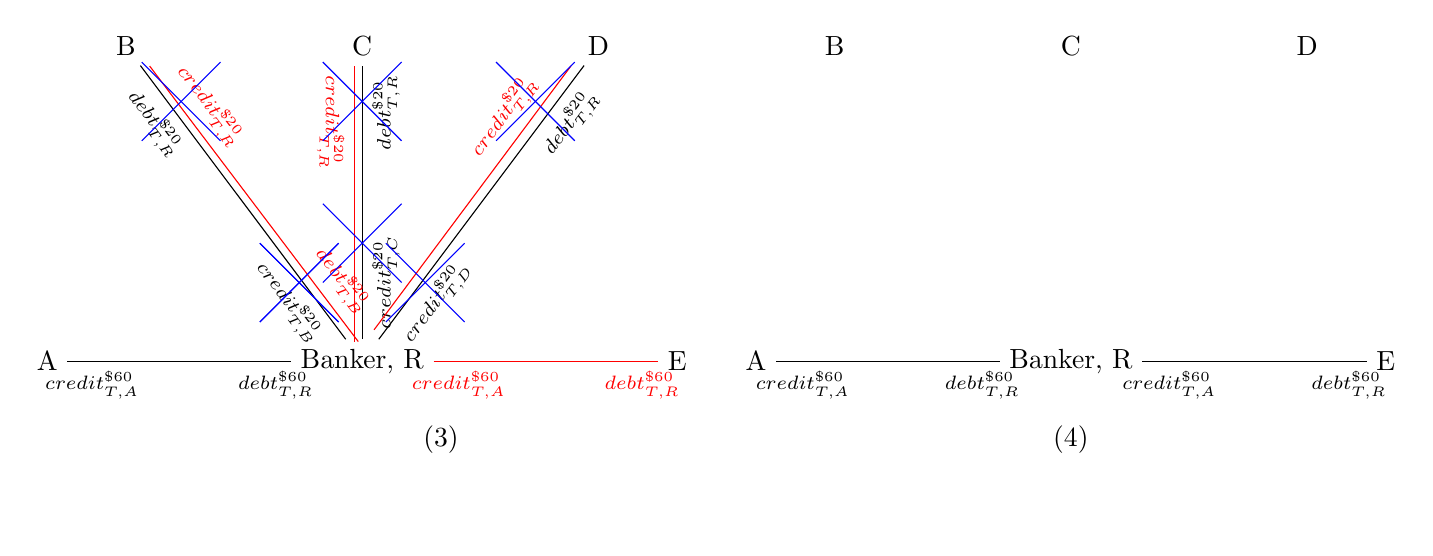
\begin{tikzpicture}
  \draw[help lines,white] (0,0) grid (17,4);
  \node         (A1)         at (0,0) {A};
  \node         (B1)         at (1,4) {B};
  \node         (C1)         at (4,4) {C};
  \node         (D1)         at (7,4) {D};
  \node         (b1)         at (4,0) {Banker, R};
  \node         (E1)         at (8,0) {E};
  \begin{scope}[every node/.style={midway,auto,font=\scriptsize}]
    \draw[black] (b1)   -- node [sloped,below] 
                {$debt^{\$20}_{T,R}$ \hspace{.62in} $credit^{\$20}_{T,B}$} (B1);
     \draw[black] (b1)   -- node [sloped,below] 
                {$credit^{\$20}_{T,C}$ \hspace{.35in} $debt^{\$20}_{T,R}$} (C1);
     \draw[black] (b1)   -- node [sloped,below] 
                {$credit^{\$20}_{T,D}$ \hspace{.62in} $debt^{\$20}_{T,R}$} (D1);
     \draw[black] (b1)   -- node [sloped,below] 
                {$credit^{\$60}_{T,A}$ \hspace{.42in} $debt^{\$60}_{T,R}$} (A1);
     \draw[red] (b1)   -- node [sloped,below] 
                {$credit^{\$60}_{T,A}$ \hspace{.42in} $debt^{\$60}_{T,R}$} (E1);
     \draw[red] (1.3,3.75) -- (3.95,.25) node[sloped,above]  
                          {$credit^{\$20}_{T,R}$ \hspace{.6in} $debt^{\$20}_{T,B}$};
     \draw[red] (3.9,3.75) -- (3.9,.25) node[sloped,below]  
                          {$credit^{\$20}_{T,R}$ \hspace{.7in} \space\space};
     \draw[red] (6.65,3.75) -- (4.15,.4) node[sloped,above]  
                          {\space\space \hspace{.8in} $credit^{\$20}_{T,R}$ };
  \end{scope}
  \draw[blue] (1.2,2.8)   -- (2.2,3.8);
  \draw[blue] (1.2,3.8)   -- (2.2,2.8);
  \draw[blue] (3.5,2.8)   -- (4.5,3.8);
  \draw[blue] (3.5,3.8)   -- (4.5,2.8);
  \draw[blue] (5.7,2.8)   -- (6.7,3.8);
  \draw[blue] (5.7,3.8)   -- (6.7,2.8);
  \draw[blue] (2.7,0.5)   -- (3.7,1.5);
  \draw[blue] (2.7,1.5)   -- (3.7,.5);
  \draw[blue] (2.7,0.5)   -- (3.7,1.5);
  \draw[blue] (2.7,1.5)   -- (3.7,.5);
  \draw[blue] (4.3,0.5)   -- (5.3,1.5);
  \draw[blue] (4.3,1.5)   -- (5.3,.5);
  \draw[blue] (3.5,1)     -- (4.5,2);
  \draw[blue] (3.5,2)     -- (4.5,1);
  \node         (A2)         at (9,0) {A};
  \node         (B2)         at (10,4) {B};
  \node         (C2)         at (13,4) {C};
  \node         (D2)         at (16,4) {D};
  \node         (b2)         at (13,0) {Banker, R};
  \node         (E2)         at (17,0) {E};
  \begin{scope}[every node/.style={midway,auto,font=\scriptsize}]
     \draw[black] (b2)   -- node [sloped,below] 
                {$credit^{\$60}_{T,A}$ \hspace{.4in} $debt^{\$60}_{T,R}$} (A2);
     \draw[black] (b2)   -- node [sloped,below] 
                {$credit^{\$60}_{T,A}$ \hspace{.4in} $debt^{\$60}_{T,R}$} (E2);
  \end{scope}
  \node at (5,-1)  {(3)};
  \node at (13,-1) {(4)};
  \node at (5,-2)  {\space};
\end{tikzpicture}
\caption[Debt-credit relationships with banker $R$, making loans]%
{Debt-credit relationships with banker $R$, making loans\par\vspace{.05in}(1): $B$, $C$ and $D$ make an agreement with the banker $R$, by which he undertakes to become the debtor of $A$ in their place, while they at the same time agree to become the debtors of the banker. Then, $B$, $C$ and $D$ make their purchases from $A$, \$20 worth each, and instead of giving to $A$ their acknowledgements of debt they give him an acknowledgement of debt of the banker $R$. As a result, the banker $R$ holds credits on $B,C,D$ of \$20 worth each and \$60 debts to $A$. \par (2): Now, $B$, $C$ and $D$ sell goods to $E$, \$20 worth each, to $E$ via the same arrangement. As a result, $B$, $C$ and $D$ have credits on $R$ of \$20 value, while $R$ has additional credits on $E$ of \$60 value. \par (3): $B$,$C$, and $D$ pay on their past debt with the banker $R$ by offseting their debts to $R$ with credits on $R$ as they are of the same due date and value. \par (4): As a result, after having their purchases and sales $B$,$C$, and $D$ have no debts and credits, while $A$, $E$ and $R$ retain their debt-credit relationships.}
\label{fig:bank_clearing_house2}
\vspace{.2in}
\end{figure}

In the case of making loans, the banker anticipated the purchase and sale transactions and made the following agreements with the counter parties. That is instead of buyers becoming debtors to the sellers and, vice versa, sellers becoming creditors to the buyers, it was the banker that had to become debtor to the sellers and creditor to the buyers. See Figure~\ref{fig:bank_clearing_house2} on p.~\pageref{fig:bank_clearing_house2}. Hence, instead of buying bills from the creditors and after the purchase-sale transactions, as shown in the above Figure~\ref{fig:bank_clearing_house1}, the banker is proactive. It is the banker's bills, which the buyers obtain from her, to hand over to the seller. ``These bills of
exchange on a banker are called cheques or drafts"~\citep[p.~403]{innes1913}. As the banker proactively anticipates many, and then majority, of such transactions then accumulates mutual debt-credit relationships of opposite type with her counter parties. And when these mutual debt-credit pairs are of same value and due date, then once due date arrived on the banker's debts she used the set-off principle of payment, which is offsetting the due debts with due credits with respect to a particular counter party, or parties. As shown in Figure~\ref{fig:bank_clearing_house2}, for example, the banker \textit{R} had mutual debt-credit relationships with individuals \textit{B,C,D}. These were set off on the due date of $T$ and these names were dropped from the accounting books of the banker. Similarly, set-off worked for \textit{B,C,D}.
  
Also, bankers centralized on themselves the operations of the governing authority of the land.  Even though the clearing house operations were conducted by authorities themselves as it was the case in England (see above), "from the earliest days of history \dots [the bankers] were always the financial agents of the governments"~\citep[p.~399]{innes1913}. And tax paying public utilized banks that allowed them to make the payment that was due. The bankers anticipated the public want of credits on the government, hence, they were discounting those from original creditors of the government.

However, the key innovation of banks as becoming the clearing houses of commercial and government-related debt and credits was intensification of the payment via the set-off principle. This allowed the banks to shift payments from periodic to immediate set-off. It had an effect in terms: (i) increased centralization, (ii) widened participation of community members in the commercial activities, and (iii) increased regularity or frequency. The set-off principle now  

\begin{quote}
\dots in practice it is not necessary for a
 debtor to acquire credits on the same persons to whom he is debtor. \dots by the wonderfully efficient machinery of the banks to which we sell our credits, and which thus
 become the clearing houses of commerce, the debts and credits of the
 whole community are centralised and set off against each other. In
 practice, therefore, any good credit will pay any debt.~\citep[p.~152]{innes1914}
\end{quote}

In case of centralization it meant that a bank became a counter-party to many members of the community and hence for a debtor it was much easier to find credits on the bank to offset her debts that were due. Instead of finding credits on a specific creditor, it became enough to obtain credits on the banker. The bankers turned the previously personalized debt-credit pairs into quasi-impersonal ones, where the banker was a side to the debt-credit pair either on the side of debtor or on the opposite side of creditor. In case of frequency the debt settlements shifted towards a daily and possibly intraday occurrence instead of the long periods, between fairs. Hence, the bankers became speacialists in shaping the debt-credit relationships. However, not in all of them as government's creation of the debt-credit pairs, where it hold tax credits on the public, was an assential and yet a separate matter.

\begin{quote}
Debts and credits are perpetually trying to get into touch with one
 another, so that they may be written off against each other, and it is the
 business of the banker to bring them together. \dots
There is thus a constant circulation of debts and credits through the
 medium of the banker who brings them together and clears them as the
 debts fall due.~\citep[pp.~402-403]{innes1913} 
\end{quote}

In the quote above \citeauthor{innes1913} used ``cirulation" word for debts and ctedits. It was a casual usage that should not distract from the details on how the bankers had became such active clearing houses so that they were performing this function on a ``constant" manner. In other words, they have been doing payments most of the time they were open to business until they were not. In the United States, during the financial panics of 1893 and 1907, banks did suspend payments. Normal, i.e. panic-free, operations of banks as centralized clearing houses is based upon the following description:

\begin{quote}\label{innes_on_good_banker}
The object of every good banker\index{Mitchell Innes, Alfred!on good banker} is to see that at the end of each day's operations, his debts to other bankers do not exceed his credits on those bankers, and in addition the amount of the ``lawful money" or credits on the government in his possession. This requirement limits the amount of money he has to ``lend." He knows by experience pretty accurately the amount of the cheques he will have to present for payment to other bankers and the amount of those which will be presented for his payment, and he will refuse to buy bills or to lend money---that is to say, he will refuse to incur present obligations in return for future payments---if by so doing he is going to risk having more debts due by him on a certain day than he will have credits on that day to set against them. \textit{It must be remembered that a credit due for payment at a future time cannot be set off against a debt due to another banker immediately. Debts and credits to be set off against each other must be 'due' at the same time.}~\citep[p.~403, emphasis added]{innes1913} 
\end{quote}

The above lengthy quote gives us an idea what is at stake with payments for the banker. The banker, which as it was discussed above had centralized the debt-credit relationship creation, re-use and their set-off on herself, innovated farther. The key of bankers' innovation was that they created and maintained such debt-credit relationships which were due today, which is to say immidiately or presently, on the continious basis. In other words, the banker maintained debt-credit pairs that due today \textit{continiously}. 

When \citeauthor{innes1913} says that the banker ``will refuse to buy bills or to lend money---that is to say, he will
refuse to incur present obligations in return for future payments" he was speaking of that advancedment with respec to the practice of discounting bills and making loans, which was first depicted in Figures~\ref{fig:bank_clearing_house1} and \ref{fig:bank_clearing_house2} above, pp.~\pageref{fig:bank_clearing_house1}-\pageref{fig:bank_clearing_house2}. In those depictions banker's \acfp{dcr} with the counter parties were dated to match the debt-credit pairs those very counter parties would establish themselves, while buying and selling to each other. In the quote above, the banker's role is being presented in a more sophisticated role. That is the banker induced discounting bill and making loans by offering to the counter party, which is on the creditor side of the \acf{dcr}, a special type of the relationship. The latter was of the type which is due today or, interchangably: immediately, presently, or on demand. By this, the banker was offering to be on the creditor side of the dated \ac{dcr}, while being on the debtor side of the \ac{dcr} due today continiously. The incentive for banker's counter parties to have \acp{dcr} due today continiously was that they could use credits on the banker due today to set-off\index{Set-off} against the debts coming due today and on every tomorrow.  See Figures~\ref{fig:bank_ds_bill}-\ref{fig:bank_mk_loan} below, on pp.~\pageref{fig:bank_ds_bill}-\pageref{fig:bank_mk_loan}. 

Then, the relational posotions between a banker and her customer can be presented by the balance sheets, which feature two types of \acfp{dcr} dated and due today continiously. See Figure~\ref{fig:bs_bnk_indv} on p.~\pageref{fig:bs_bnk_indv}. 

\begin{figure}[!ht]
\centering
\vspace{.3in}
\captionsetup{width=.9\linewidth,labelfont=bf}
\usetikzlibrary {matrix}
\begin{tikzpicture}
  \draw[help lines,white] (0,0) grid (15,6);
  % Left-hand side part of the Figure
  \node         (A)         at (1,4.5) {A};
  \node         (R)         at (6,4.5) {R};
  \node         (B)         at (3.5,0.5) {B};
  \node                     at (3.5,-.5) {(1)};  
  \draw (A) -- (B) node[midway,sloped,above]%
        {\textsuperscript{\textit{debt: }$d^{\$}_{t,B}$ \hspace{.55in} $credit: d^{\$}_{t,A}$}};
  \draw[dashed,blue] (A) .. controls +(left:1.2cm) and +(left:2cm) .. 
                       node[below,sloped]%
                       {\textsuperscript{$A$ bought goods from $B$}} (B);
    \draw[dashed,red] (R) .. controls +(right:1.2cm) and +(right:2cm) .. 
                       node[below,sloped]%
                       {\textsuperscript{$R$ buys dated credit from $B$}} (B);
  % Right-hand side part of the Figure
  \node         (A)         at (9,4.5) {A};
  \node         (R)         at (14,4.5) {R};
  \node         (B)         at (11.5,0.5) {B};
  \node                     at (11.5,-.5) {(2)};
  \draw (A) -- (R) node[midway,sloped,above]%
        {\textsuperscript{\textit{debt: }$d^{\$}_{t,R}$ \hspace{.6in} $credit: d^{\$}_{t,A}$}};
  \draw[thick] (B) -- (R) node[midway,sloped,below]%
        {\textsuperscript{$credit: \overrightarrow{c^{\$}_{0,R}}$ \hspace{.45in} $debt: \overrightarrow{d^{\$}_{0,B}}$}};
\end{tikzpicture}
\caption[Banker by discounting bill creates new debt-credit pair due today]%
{Banker by discounting bill creates new debt-credit pair due today\par\vspace{.05in}(1): Banker $R$ finds an existing dated debt-credit pair between $A$ and $B$, which is due in $t$ days. $R$ considers attractive having a dated credit on $A$, because $A$ is perceived capable selling goods herself and obtain credits on others. Hence, $R$ approached $B$ by offering a swap: $B$'s dated credit on $A$ for $B$'s credit due today on $R$. $B$'s interest is having such a swap is that she can use credit due today to use set-off principle against her other debt that coming due today or tomorrow, which is to make payment due today. Lastly, $R$ buys $B$'s credit on $A$ this way.\par (2): Now, after $B$ handed over $A$'s acknowledgement of debt to $R$, $A$ is dated debtor to $R$ and the latter is dated creditor of the former, while $B$ holds credit due today on $R$ and the latter owed debt due today to $B$.}
\label{fig:bank_ds_bill}
\vspace{.2in}
\end{figure}

\begin{figure}[!ht]
\centering
\vspace{.3in}
\captionsetup{width=.9\linewidth,labelfont=bf}
\usetikzlibrary {matrix}
\begin{tikzpicture}
  \draw[help lines,white] (0,0) grid (15,6);
  % Left-hand side part of the Figure
  \node         (A)         at (1,4.5) {A};
  \node         (R)         at (6,4.5) {R};
  \node         (B)         at (3.5,0.5) {B};
  \node                     at (3.5,-.5) {(1)};
  \draw[black]   (A.north) |- (4,5) -| (R.north);
  \draw[black,thick]   (A.south) |- (4,4) -| (R.south);
  \node at (3.5,5.4) {\textsuperscript{\textit{debt: }$d^{\$}_{t,R}$ \hspace{.7in} \textit{credit: }$d^{\$}_{t,A}$}};
  \node at (3.5,3.6) {\textsuperscript{\textit{credit: }$\overrightarrow{c^{\$}_{0,R}}$ \hspace{.7in} \textit{debt: }$\overrightarrow{d^{\$}_{0,A}}$}};  
  \draw[dashed,blue] (A) .. controls +(left:-3cm) and +(left:-1.5cm) .. 
                       node[above,sloped]%
                       {\textsuperscript{$A$ buys from $B$}} (B);
  \draw (A) -- (0,3.5) -- (B); 
  \node[rotate=49] at (.2,4) {\textsuperscript{\textit{debt: }$d^{\$}_{0,B}$}};
  \node[rotate=-40] at (2.4,1) {\textsuperscript{\textit{credit: }$c^{\$}_{0,A}$}};
  % Right-hand side part of the Figure
  \node         (A)         at (9,4.5) {A};
  \node         (R)         at (14,4.5) {R};
  \node         (B)         at (11.5,0.5) {B};
  \node                     at (11.5,-.5) {(2)};
  \draw (A) -- (R) node[midway,sloped,above]%
        {\textsuperscript{\textit{debt: }$d^{\$}_{t,R}$ \hspace{.6in} $credit: d^{\$}_{t,A}$}};
  \draw[thick] (B) -- (R) node[midway,sloped,below]%
        {\textsuperscript{$credit: \overrightarrow{c^{\$}_{0,R}}$ \hspace{.45in} $debt: \overrightarrow{d^{\$}_{0,B}}$}};
\end{tikzpicture}
\caption[Banker by making loan creates two debt-credit pairs]%
{Banker by making loan creates two debt-credit pairs: dated and due today\par\vspace{.05in}(1): Banker $R$ makes loan with $A$ by establishing two debt-credit pairs with each other: one is dated (thin line) and one is due today (thick line). $A$'s prime interest with $R$ is to buy from $B$ some good or service. \par (2): $A$ uses credit on $R$ as payment to $B$ by either handing $R$'s acknowledgement of debt over to $B$ or by instructing $R$ to assign her debt to $A$ to $B$.}
\label{fig:bank_mk_loan}
\vspace{.2in}
\end{figure}

\begin{figure}[!ht]
\captionsetup{width=.9\linewidth,labelfont=bf}
  \vspace{.4in}
  \centering
  \begin{tikzpicture}
  \draw[help lines,white] (0,0) grid (16,8);
        %
        % Banker R ---------------------------------------------------------
        \matrix (m) [matrix anchor=north, matrix of nodes, nodes in empty cells,
             nodes = {text width=2.5in, minimum height=.2in, align=left},
             column sep=1em,
             row 2/.style={align=center, font=\bfseries},
            ] at (8,8)
        {
         & \\
        Assets: total credits ($\mathbf{c^{\$}_t}$) & Liabilities: total debts ($\mathbf{d^{\$}_t}$) \\
        $\overrightarrow{c_{0}}$: credits due today continuously & $\overrightarrow{d_{0}}$: debts due today continuously \\
        $c_{\tiny t}$: dated credits, ($t \geq 0$) & $d_{\tiny t}$: dated debts, ($t \geq 0$) \\
         };
        \node[fit=(m-1-1)(m-1-2)]%
        {\textit{\MakeUppercase{Banker's (R) positions}}};
        \draw[thin]  (m-2-2.south -| m.west) -- (m-2-2.south -| m.east);
        \draw[thin]  (m-1-1.south east) -- (m-4-1.south east);       
        %
        % Individual A -----------------------------------------------------
        \matrix [matrix anchor=north, matrix of nodes, nodes in empty cells,
             nodes = {text width=2.5in, minimum height=.2in, align=left},
             column sep=1em,
             row 2/.style={align=center, font=\bfseries},
            ] (n) at (8,4) 
        {
         & \\
        Assets: total credits ($\mathbf{c^{\$}_t}$) & Liabilities: total debts ($\mathbf{d^{\$}_t}$) \\
        $\overrightarrow{c_{0}}$: credits due today continuously & $d_{0}$: debts due today \\
        $c_{\tiny t}$: dated credits, ($t \geq 0$) & $d_{\tiny t}$: dated debts, ($t>0$) \\
         };
        \node[fit=(n-1-1)(n-1-2)]%
        {\textit{\MakeUppercase{Private individual's (A) positions}}};
        \draw[thin]  (n-2-2.south -| n.west) -- (n-2-2.south -| n.east);
        \draw[thin]  (n-1-1.south east) -- (n-4-1.south east);
  \end{tikzpicture}
 \caption[Typical balance sheets of a banker and a private individual, banker's customer]%
  {Typical balance sheets of a banker and private individual\par \vspace{.05in}Both of them contain only relational positions in the debt-credit pairs, being established by (a) purchase and sale transactions, and (b) levying tax by the government. Debts and credits are denominated in a single money of account such as dollar (\$) and they grouped by maturity/tenor type: (1) due today continuously $\overrightarrow{d_{0}}$ and $\overrightarrow{c_{0}}$, and (2) dated or due at some later day $d_t$ and $c_t$, where $t$ means number of days between today and the due date, when that debt-credit pair was originally created. Note that $\overrightarrow{d_{0}}$ and $d_0$ of same nominal value and owed to the same counter party are different types of debts. The former is due today continuously, while the latter happened to be due today because its due date has arrived. It is similar with $\overrightarrow{c_{0}}$ and $c_0$.}
  \label{fig:bs_bnk_indv}
\end{figure}

Thus, when the banker discounts bills or makes loan, she increases the size of dated credits she holds -- these are promises from her customers of ``future payments" in her favor that \citeauthor{innes1913} was talking about in the quote above. At the same time, the banker incurs ``present obligations," which are her debts due today continuously she owes to her customers. 

For example, when banker \textit{R} makes loan with \textit{A}, as in secion (1) of Figure \ref{fig:bank_mk_loan}, her dated credits on \textit{A} in the assets side of the balance sheet rise by the size of the loan, while in her liabilities it is the debts due today to \textit{A} that increase by the same amount. The balance sheet of \textit{A}, too, records these two \acfp{dcr} in opposite manner: credits due today on the banker \textit{R}, which are in the assets, do increase, while in the liabilities it is dated debts owed to \textit{R} that increase. Consider these changes in the relational positions through the exposition of balance sheets in Figure~\ref{fig:bs_bnk_indv}, p.~\pageref{fig:bs_bnk_indv}.

Now, \textit{A} is able to make a payment on her purchase of goods from the individual \textit{B}. If the latter agrees to hold the banker \textit{R} debts due today, then the payment from \textit{A} to \textit{B} proceeds immediately this way. Since \textit{A} is the buyer she becomes debtor to \textit{B}, who is the seller turning creditor to \textit{A} albeit for a moment. \textit{A} has debt due today to \textit{B}, which she offsets with credit due today on the banker \textit{R}. \textit{A} either (i) hands over the banker's acknowledgement of debt, if it is tangable bill or checque or draft, to \textit{B} without letting know \textit{R} of this development, or (ii) instructs \textit{R} directly to liquidate her debt due today and owed to \textit{A} and then immediately assign debt due today of the same size in favor of \textit{B}, which is concluded by \textit{R} through letting know of \textit{B} of this development. This result of the debt-credit pairs change is depicted in section (2) of Figure \ref{fig:bank_mk_loan}.

Exending the above example, the following discussion shows how \textit{A} utilizies set-off principle in its complete form to liberate herself from debt to the banker \textit{R}, which is due in \textit{t} days. Review Figure~\ref{fig:bank_mk_loan2} on p.~\pageref{fig:bank_mk_loan2} along the description that follows below. Recall that by selling individuals acquire credits. It is assumed that new individual \textit{C} is interested in buying goods from \textit{A}. Hence, by selling \textit{A} will acquire credits to pay on her past debt to the banker \textit{R}. Aslo, recall that it was the banker calculation from the very beginning that \textit{A} is capable in selling. Now, another crucial assumption is that banker \textit{R} agrees to make loan to \textit{C} in order to buy from \textit{A}. The banker's calculation is similar that she anticipates \textit{C} to be good in future selling and acquiring credits. The size of loan to \textit{C} is equal to the \textit{A}'s indebtedness with the banker -- this is simplified the exposition of the set-off. Hence, as \textit{C} engages into loan agreement with banker, she buys goods from \textit{A} and becomes debtor to the latter just for a moment. \textit{C} utilizes the partial set-off for her debt to \textit{A} by matching it with credit on \textit{R}, whereas \textit{A} swaps her position with banker on whom she now holds credit due today. This is shown in section (3) of Figure~\ref{fig:bank_mk_loan2}. As a result, \textit{A} has debt to banker that is due in \textit{t} days and credit on the same banker which is due today continuously. These debt and credit are mutual, of the same nominal worth and denominated in same money of account, while due dates are different. Hence, it is only when \textit{A}'s debt to the banker becomes due---when \textit{t} runs down to zero or the due date becomes today---the complete set-off principle is applied by both sides, which are individual \textit{A} and banker \textit{R}. Both of them offset those debts and credits on each other within own books. Their mutual and oppostite \acp{dcr} are ``cleared." This is shown in section (4) of Figure~\ref{fig:bank_mk_loan2}.

\begin{figure}[!ht]
\centering
\vspace{.0in}
\captionsetup{width=.9\linewidth,labelfont=bf}
\usetikzlibrary {matrix}
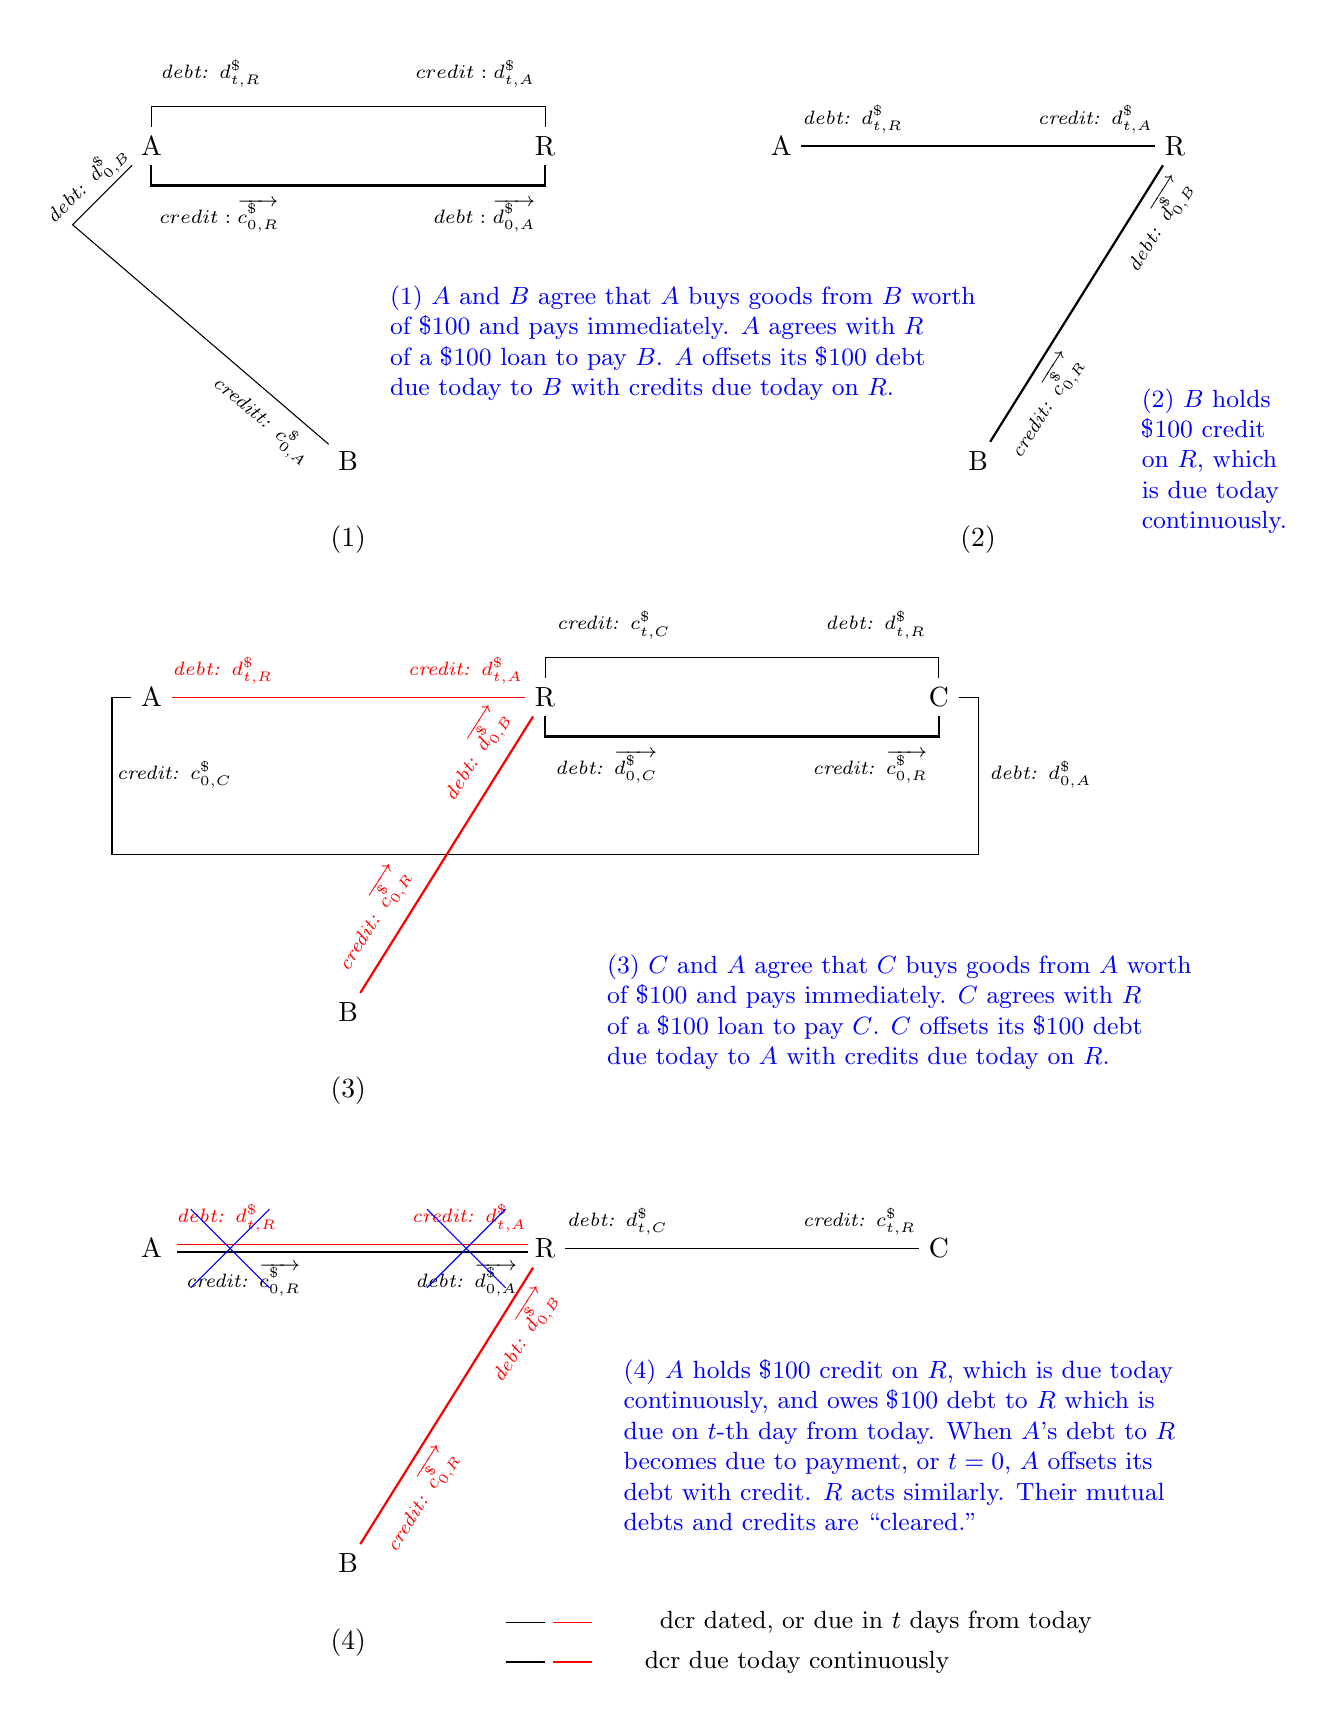
\begin{tikzpicture}
  \draw[help lines,white] (0,0) grid (14,21);
  % Left-hand side part of the Figure
  \node         (A)         at (1,19.5) {A};
  \node         (R)         at (6,19.5) {R};
  \node         (B)         at (3.5,15.5) {B};
  \node                     at (3.5,14.5) {(1)};
  \draw[black]   (A.north) |- (4,20) -| (R.north);
  \draw[black,thick]   (A.south) |- (4,19) -| (R.south);
  \draw (A) -- (0,18.5) -- (B); 
  \node[rotate=45] at (.2,19) {\textsuperscript{\textit{debt: }$d^{\$}_{0,B}$}};
  \node[rotate=-40] at (2.4,16) {\textsuperscript{\textit{creditt: }$c^{\$}_{0,A}$}};
  \node at (3.5,20.4) {\textsuperscript{\textit{debt: }$d^{\$}_{t,R}$ \hspace{.7in} $credit: d^{\$}_{t,A}$}};
  \node at (3.5,18.6) {\textsuperscript{$credit: \overrightarrow{c^{\$}_{0,R}}$ \hspace{.7in} $debt: \overrightarrow{d^{\$}_{0,A}}$}};  
  %\draw[dashed,blue] (A) .. controls +(left:1.2cm) and +(left:2cm) .. (B);
        %node[below,sloped,font=\small] {$A$ buys goods from $B$} (B);
  \node[blue,align=left,font=\small] at (7.75,17) {(1) $A$ and $B$ agree that $A$ buys goods from $B$ worth \\of \$100 and pays immediately. $A$ agrees with $R$\\of a \$100 loan to pay $B$. $A$ offsets its \$100 debt\\due today to $B$ with credits due today on $R$.}; 
  \node[blue,align=left,font=\small] at (14.5,15.5) {(2) $B$ holds\\ \$100 credit\\on $R$, which\\is due today\\continuously.};
  % Right-hand side part of the Figure
  \node         (A)         at (9,19.5) {A};
  \node         (R)         at (14,19.5) {R};
  \node         (B)         at (11.5,15.5) {B};
  \node                     at (11.5,14.5) {(2)};
  \draw (A) -- (R) node[midway,sloped,above]%
        {\textsuperscript{\textit{debt: }$d^{\$}_{t,R}$ \hspace{.6in} \textit{credit: }$d^{\$}_{t,A}$}};
  \draw[thick] (B) -- (R) node[midway,sloped,below]%
        {\textsuperscript{\textit{credit: }$\overrightarrow{c^{\$}_{0,R}}$ \hspace{.45in} \textit{debt: }$\overrightarrow{d^{\$}_{0,B}}$}};
  % Middle part of the Figure
  \node         (A)         at (1,12.5) {A};
  \node         (R)         at (6,12.5) {R};
  \node         (B)         at (3.5,8.5) {B};
  \node         (C)         at (11,12.5) {C};
  \node                     at (3.5,7.5) {(3)};
  %\draw[dashed,blue] (A) to [out=-30,in=-30] node[sloped,below,font=\small]        {$C$ buys goods from $A$} (C);
  \draw[black]   (C.north) |- (10,13) -| (R.north);
  \draw[black,thick]   (C.south) |- (10,12) -| (R.south);
  \draw (A.west) -- (.5,12.5) |- (5,10.5) -| (11.5,12.5) -- (C.east);
  \node[align=left] at (1.3,11.5) {\textsuperscript{\textit{credit: }$c^{\$}_{0,C}$}};
  \node[align=left] at (12.3,11.5) {\textsuperscript{\textit{debt: }$d^{\$}_{0,A}$}};
  \node at (8.5,13.4) {\textsuperscript{\textit{credit: }$c^{\$}_{t,C}$ \hspace{.7in} \textit{debt: }$d^{\$}_{t,R}$}};
  \node at (8.5,11.6) {\textsuperscript{\textit{debt: }$\overrightarrow{d^{\$}_{0,C}}$ \hspace{.7in} \textit{credit: }$\overrightarrow{c^{\$}_{0,R}}$}}; 
  %\draw[red,thick] (B) -- (R);
  \draw[red] (A) -- (R) node[midway,sloped,above]        {\textsuperscript{\textit{debt: }$d^{\$}_{t,R}$ \hspace{.6in} \textit{credit: }$d^{\$}_{t,A}$}};
  \draw[red,thick] (B) -- (R) node[midway,sloped,above]%
        {\textsuperscript{\textit{credit: }$\overrightarrow{c^{\$}_{0,R}}$ \hspace{.35in} \textit{debt: }$\overrightarrow{d^{\$}_{0,B}}$}};
  \node[blue,align=left,font=\small] at (10.5,8.5) {(3) $C$ and $A$ agree that $C$ buys goods from $A$ worth \\of \$100 and pays immediately. $C$ agrees with $R$\\of a \$100 loan to pay $C$. $C$ offsets its \$100 debt\\due today to $A$ with credits due today on $R$.};
  % Bottom part of the Figure
  \node         (A)         at (1,5.5) {A};
  \node         (R)         at (6,5.5) {R};
  \node         (B)         at (3.5,1.5) {B};
  \node         (C)         at (11,5.5) {C};
  \node                     at (3.5,0.5) {(4)};
  %\draw[red] (A) -- (R) node[midway,sloped,above]
  \draw[red] (1.32,5.55) -- (5.78,5.55) node[midway,sloped,above] {\textsuperscript{\textit{debt: }$d^{\$}_{t,R}$ \hspace{.6in} \textit{credit: }$d^{\$}_{t,A}$}};
  \draw[thick] (1.32,5.45) -- (5.78,5.45)  node[midway,sloped,below]%
        {\textsuperscript{\textit{credit: }$\overrightarrow{c^{\$}_{0,R}}$ \hspace{.5in} \textit{debt: }$\overrightarrow{d^{\$}_{0,A}}$}};
  \draw[black] (C) -- (R) node[midway,sloped,above] {\textsuperscript{\textit{debt: }$d^{\$}_{t,C}$ \hspace{.6in} \textit{credit: }$c^{\$}_{t,R}$}};
  \draw[red,thick] (B) -- (R) node[midway,sloped,below]%
        {\textsuperscript{\textit{credit: }$\overrightarrow{c^{\$}_{0,R}}$ \hspace{.35in} \textit{debt: }$\overrightarrow{d^{\$}_{0,B}}$}};
   \draw[blue] (1.5,5)   -- (2.5,6);
   \draw[blue] (1.5,6)   -- (2.5,5);
   \draw[blue] (4.5,5)   -- (5.5,6);
   \draw[blue] (4.5,6)   -- (5.5,5);
   \node[blue,align=left,font=\small] at (10.5,3) {(4) $A$ holds \$100 credit on $R$, which is due today\\continuously, and owes \$100 debt to $R$ which is\\due on $t$-th day from today. When $A$'s debt to $R$\\becomes due to payment, or $t=0$, $A$ offsets its\\debt with credit. $R$ acts similarly. Their mutual\\debts and credits are ``cleared."};
   % Labels
  %\draw[black] (5.5,.75) -- (6.5,.75); 
  \draw[black] (5.5,.75) -- (6,.75);\draw[red] (6.1,.75) -- (6.6,.75); 
  \node[black,align=left,font=\small] at (10.2,.75) {\ac{dcr} dated, or due in $t$ days from today};
  %\draw[black,thick] (5.5,0.25) -- (6.5,0.25) 
  \draw[black,thick] (5.5,0.25) -- (6,0.25);\draw[red,thick] (6.1,0.25) -- (6.6,0.25); 
  \node[black,font=\small] at (9.2,0.25) {\ac{dcr} due today continuously};
\end{tikzpicture}
\caption[Banker $R$ makes loans to facilitate exchange between $A,B,C$]%
{Banker $R$ makes loans to facilitate trade between $A,B,C$.}
\label{fig:bank_mk_loan2}
\vspace{.0in}
\end{figure}

Now, being established the principles of payment via three key methods, let us return to the \citeauthor{innes1913}' quote mentioned on p.~\pageref{innes_on_good_banker}. And in particular to his observation that a good banker may \textit{refuse} discouning of bills or making loan to an individual. This comes from the fact that banking by itself is a commercial activity. In own words by \citeauthor{innes1913}, the banker evolved the mechant activity quite simultaneously: ``Then arose the merchant or banker, the latter being merely a more specialized variety of the former." \citep[p.~403]{innes1913} If there is no harsh panishment suppreccing commerce, then community or larger society must have experience some varity of banker not only in terms of quantity. Quite crucially the population of bankers exposed to systemic and indiviual risks. The latter might range from acts of nature to individual overestimation of the clients' ability to sell or borrow and establish \acfp{dcr}, where these clients are on the credir position, and of enough worth. Hence, each such banker must had evaluated not only his clients in terms of their ability to sell and become creditors, she must had evaluated peer banker, or bankers, in terms of the latter's ability to have credits to offset own debts due. 

If, for example, bankers \textit{$R_1$} and \textit{$R_2$} might consider each other at this point of time as good credit, meaning for each it is preferable and attractive to have a \acf{dcr} with a creditor position on the other. It means, too, that in the case of payment taking place as a partial set-off then the above mentioned bankers accomodate the swap part of such a payment. Consider the example of these two bankers accomodating trade between individuals $A, B$, and $C$ as depicted in Figure~\ref{fig:bank_mk_loan3} on p.~\pageref{fig:bank_mk_loan3}. By assumption all purchases and sales are denominated in the dollar as money of account and worth \$100. This case extends the previous example depicted in Figure~\ref{fig:bank_mk_loan2} on p.~\pageref{fig:bank_mk_loan3} by allowing $C$ to borrow from banker $R_2$ the required funds to facilitate purhase of goods from $A$. This is shown by section (3) of Figure~\ref{fig:bank_mk_loan3}, where $C$ and $R_2$ establish two mutual \acfp{dcr} of different type: dated and due today continiously. In other words, $R_2$ makes loan to $C$. Since $C$ is buying from $A$ with immidiate payment, by itself it means they establish a dated \acf{dcr}, which is subject to immidiate payment ($t=0$). So, $C$ makes payment by utilizing the partial set-off by matching own debt due today to $A$ with credit due today on $R_2$ as these debt and credit are of the same worh and denominated in the same money of account. It can be said differently, as usually done, $C$ hands acknowledgement of debt on $R_2$ (in the form bill, cheque, or draft) over to $A$. On the other side of the partial set-off, $A$ swapps her creditor position on $C$ for the creditor position on $R_1$, which extends this swap by being on the creditor position on $R_2$. Lastly, on the due date of the $A$'s debt to $R_1$ both of them undertake complete set-off as they have two mutual \acp{dcr} of same worth, all due today and of same denomination. In other words their mutual debts and credits are said being ``cleared." The key point of this exposition is that bankers $R_1$ and $R_2$ ended up having a \acf{dcr} due today continuously, where the former is creditor and the latter is debtor.

This example can be extended further to show a purchase and sale transaction in the reverse direction produces $R_1$ and $R_2$ having an  opposite \acf{dcr} due today continuously. This results from $A$ buying from $D$, which is the customer of banker $R_2$. Since $A$ has no remaining balance with her banker she need to borrow from $R_1$. Her payment to $D$, which if detailed is a partial set-off with $D$ swapping her creditor position from $A$ to $R_2$ and the latter banker accomodates it by extending the swap into own creditor position on $R_1$. Eventually, $R_1$ and $R_2$ having mutual and opposie \acp{dcr} might decide to use set-off to get their debts and credits ``cleared."

\begin{figure}[!ht]
\centering
\vspace{.0in}
\captionsetup{width=1\linewidth,labelfont=bf}
\usetikzlibrary {matrix}
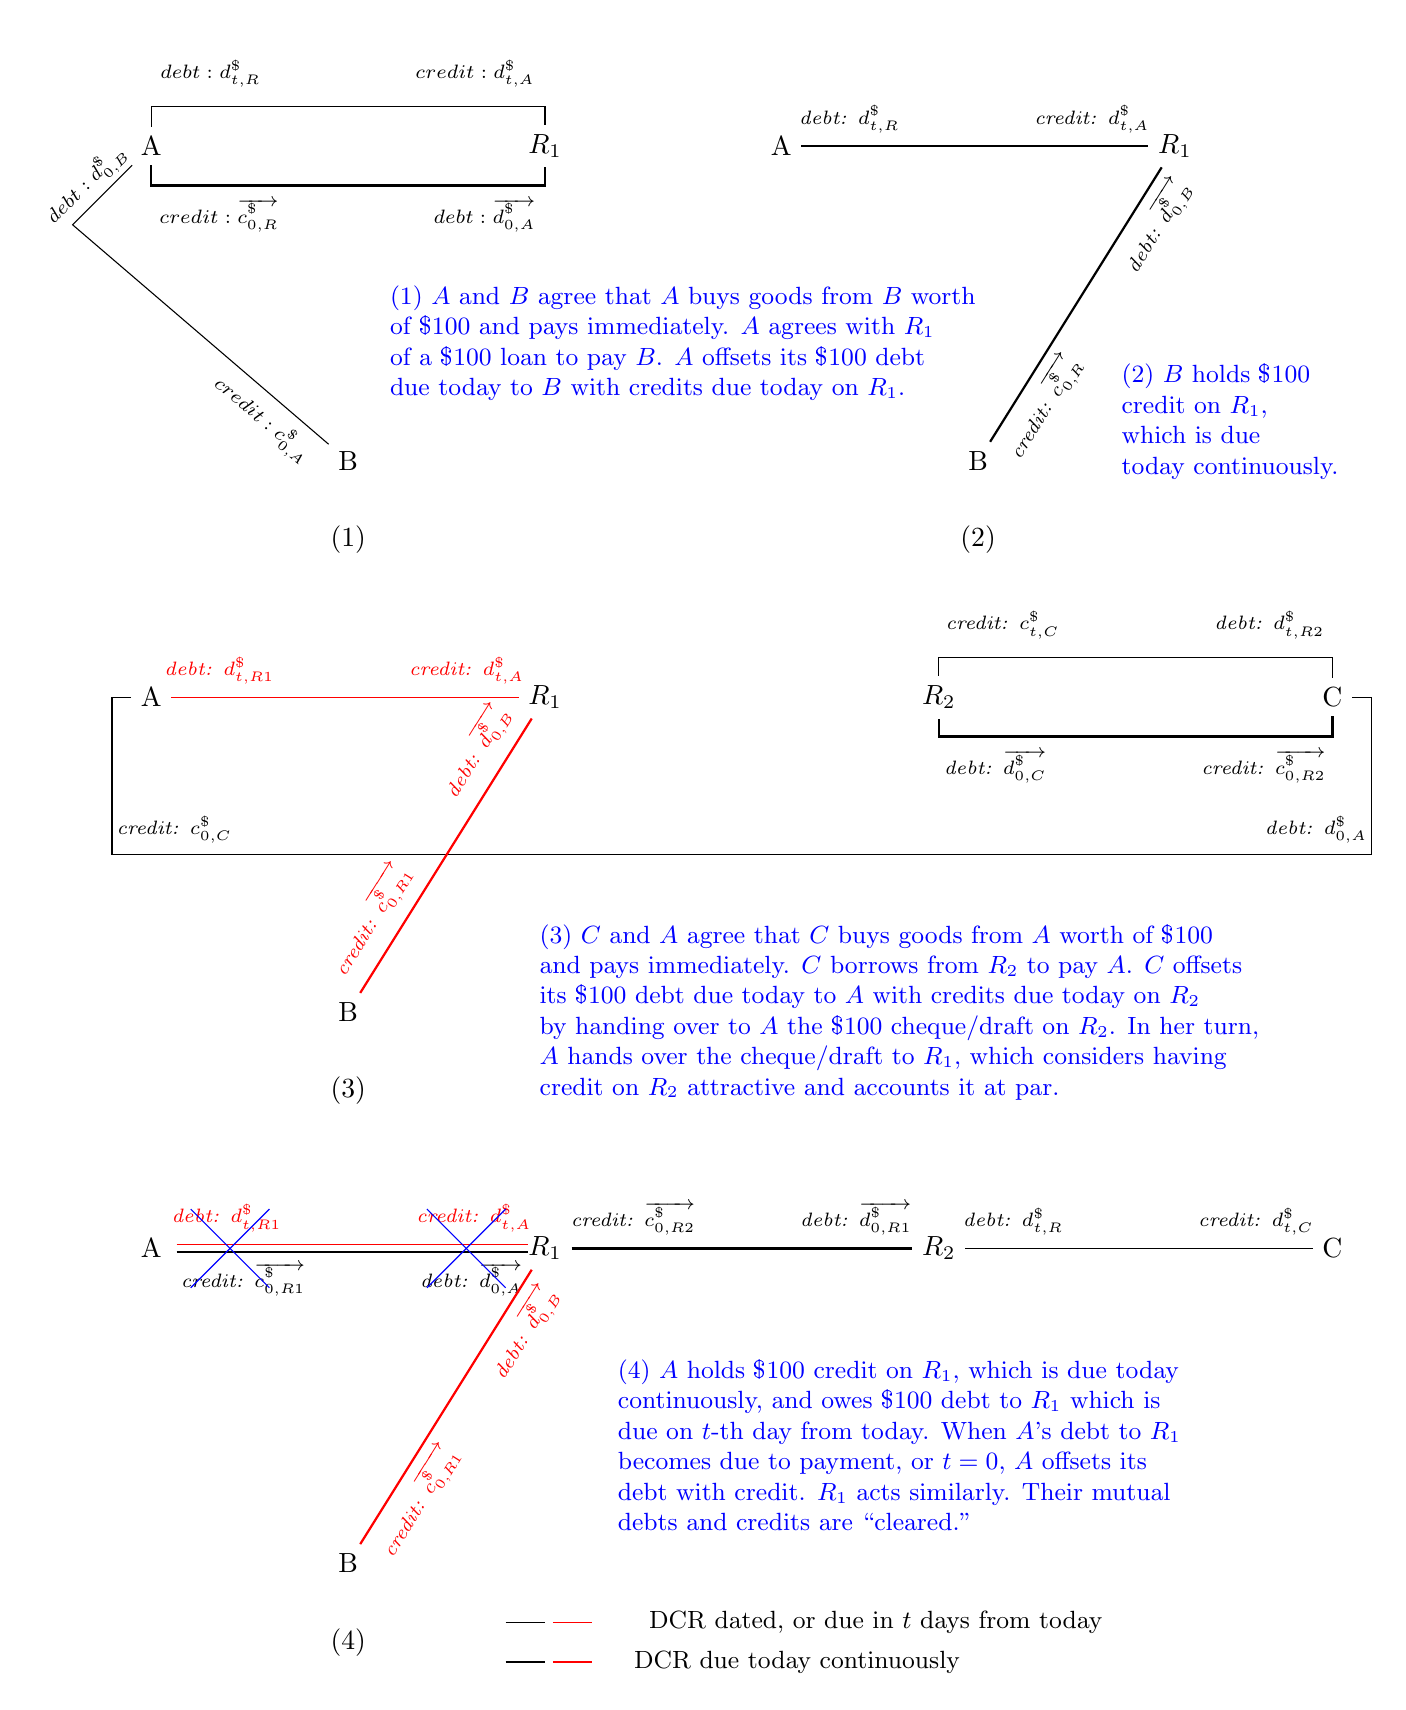
\begin{tikzpicture}
  \draw[help lines,white] (0,0) grid (16,21);
  % Left-hand side part of the Figure
  \node         (A)         at (1,19.5) {A};
  \node         (R)         at (6,19.5) {$R_1$};
  \node         (B)         at (3.5,15.5) {B};
  \node                     at (3.5,14.5) {(1)};
  \draw[black]   (A.north) |- (4,20) -| (R.north);
  \draw[black,thick]   (A.south) |- (4,19) -| (R.south);
  \draw (A) -- (0,18.5) -- (B); 
  \node[rotate=45] at (.2,19) {\textsuperscript{$debt: d^{\$}_{0,B}$}};
  \node[rotate=-40] at (2.4,16) {\textsuperscript{$credit: c^{\$}_{0,A}$}};
  \node at (3.5,20.4) {\textsuperscript{$debt: d^{\$}_{t,R}$ \hspace{.7in} $credit: d^{\$}_{t,A}$}};
  \node at (3.5,18.6) {\textsuperscript{$credit: \overrightarrow{c^{\$}_{0,R}}$ \hspace{.7in} $debt: \overrightarrow{d^{\$}_{0,A}}$}};  
  %\draw[dashed,blue] (A) .. controls +(left:1.2cm) and +(left:2cm) .. (B);
        %node[below,sloped,font=\small] {$A$ buys goods from $B$} (B);
  \node[blue,align=left,font=\small] at (7.75,17) {(1) $A$ and $B$ agree that $A$ buys goods from $B$ worth \\of \$100 and pays immediately. $A$ agrees with $R_1$\\of a \$100 loan to pay $B$. $A$ offsets its \$100 debt\\due today to $B$ with credits due today on $R_1$.};
  \node[blue,align=left,font=\small] at (14.7,16) {(2) $B$ holds \$100\\credit on $R_1$,\\which is due\\today continuously.};
  % Right-hand side part of the Figure
  \node         (A)         at (9,19.5) {A};
  \node         (R)         at (14,19.5) {$R_1$};
  \node         (B)         at (11.5,15.5) {B};
  \node                     at (11.5,14.5) {(2)};
  \draw (A) -- (R) node[midway,sloped,above]%
        {\textsuperscript{\textit{debt: }$d^{\$}_{t,R}$ \hspace{.6in} \textit{credit: }$d^{\$}_{t,A}$}};
  \draw[thick] (B) -- (R) node[midway,sloped,below]%
        {\textsuperscript{\textit{credit: }$\overrightarrow{c^{\$}_{0,R}}$ \hspace{.45in} \textit{debt: }$\overrightarrow{d^{\$}_{0,B}}$}};
  % Middle part of the Figure
  \node         (A)         at (1,12.5) {A};
  \node         (R1)        at (6,12.5) {$R_1$};
  \node         (B)         at (3.5,8.5) {B};
  \node         (R2)        at (11,12.5) {$R_2$};
  \node         (C)         at (16,12.5) {C};
  \node                     at (3.5,7.5) {(3)};
  %\draw[dashed,blue] (A) to [out=-30,in=-30] node[sloped,below,font=\small]        {$C$ buys goods from $A$} (C);
  \draw[black]   (C.north) |- (14,13) -| (R2.north);
  \draw[black,thick]   (C.south) |- (14,12) -| (R2.south);
  \draw (A.west) -- (.5,12.5) |- (5,10.5) -| (16.5,12.5) -- (C.east);
  \node[align=left] at (1.3,10.8) {\textsuperscript{\textit{credit: }$c^{\$}_{0,C}$}};
  \node[align=left] at (15.8,10.8) {\textsuperscript{\textit{debt: }$d^{\$}_{0,A}$}};
  \node at (13.5,13.4) {\textsuperscript{\textit{credit: }$c^{\$}_{t,C}$ \hspace{.7in} \textit{debt: }$d^{\$}_{t,R2}$}};
  \node at (13.5,11.6) {\textsuperscript{\textit{debt: }$\overrightarrow{d^{\$}_{0,C}}$ \hspace{.7in} \textit{credit: }$\overrightarrow{c^{\$}_{0,R2}}$}}; 
  %\draw[red,thick] (B) -- (R);
  \draw[red] (A) -- (R1) node[midway,sloped,above]        {\textsuperscript{\textit{debt: }$d^{\$}_{t,R1}$ \hspace{.6in} \textit{credit: }$d^{\$}_{t,A}$}};
  \draw[red,thick] (B) -- (R1) node[midway,sloped,above]%
        {\textsuperscript{\textit{credit: }$\overrightarrow{c^{\$}_{0,R1}}$ \hspace{.35in} \textit{debt: }$\overrightarrow{d^{\$}_{0,B}}$}};
  \node[blue,align=left,font=\small] at (10.5,8.5) {(3) $C$ and $A$ agree that $C$ buys goods from $A$ worth of \$100\\and pays immediately. $C$ borrows from $R_2$ to pay $A$. $C$ offsets\\its \$100 debt due today to $A$ with credits due today on $R_2$\\by handing over to $A$ the \$100 cheque/draft on $R_2$. In her turn,\\$A$ hands over the cheque/draft to $R_1$, which considers having\\credit on $R_2$ attractive and accounts it at par.}; %Thus, $C$\\indirectly instructs $R_2$ to assign credit of same worth due today\\continuously on $A$'s banker $R_1$.};
  % Bottom part of the Figure
  \node         (A)         at (1,5.5) {A};
  \node         (R1)        at (6,5.5) {$R_1$};
  \node         (R2)        at (11,5.5) {$R_2$};
  \node         (B)         at (3.5,1.5) {B};  
  \node         (C)         at (16,5.5) {C};
  \node                     at (3.5,0.5) {(4)};
  %\draw[red] (A) -- (R) node[midway,sloped,above]
  \draw[red] (1.32,5.55) -- (5.78,5.55) node[midway,sloped,above] {\textsuperscript{\textit{debt: }$d^{\$}_{t,R1}$ \hspace{.6in} \textit{credit: }$d^{\$}_{t,A}$}};
  \draw[thick] (1.32,5.45) -- (5.78,5.45)  node[midway,sloped,below]%
        {\textsuperscript{\textit{credit: }$\overrightarrow{c^{\$}_{0,R1}}$ \hspace{.5in} \textit{debt: }$\overrightarrow{d^{\$}_{0,A}}$}};
  \draw[black] (C) -- (R2) node[midway,sloped,above] {\textsuperscript{\textit{debt: }$d^{\$}_{t,R}$ \hspace{.6in} \textit{credit: }$d^{\$}_{t,C}$}};
  \draw[red,thick] (B) -- (R1) node[midway,sloped,below]%
        {\textsuperscript{\textit{credit: }$\overrightarrow{c^{\$}_{0,R1}}$ \hspace{.35in} \textit{debt: }$\overrightarrow{d^{\$}_{0,B}}$}};
  \draw[thick] (R1) -- (R2) node[midway,sloped,above]%
        {\textsuperscript{\textit{credit: }$\overrightarrow{c^{\$}_{0,R2}}$ \hspace{.45in} \textit{debt: }$\overrightarrow{d^{\$}_{0,R1}}$}};
   \draw[blue] (1.5,5)   -- (2.5,6);
   \draw[blue] (1.5,6)   -- (2.5,5);
   \draw[blue] (4.5,5)   -- (5.5,6);
   \draw[blue] (4.5,6)   -- (5.5,5);
   \node[blue,align=left,font=\small] at (10.5,3) {(4) $A$ holds \$100 credit on $R_1$, which is due today\\continuously, and owes \$100 debt to $R_1$ which is\\due on $t$-th day from today. When $A$'s debt to $R_1$\\becomes due to payment, or $t=0$, $A$ offsets its\\debt with credit. $R_1$ acts similarly. Their mutual\\debts and credits are ``cleared."};
   % Labels
  %\draw[black] (5.5,.75) -- (6.5,.75); 
  \draw[black] (5.5,.75) -- (6,.75);\draw[red] (6.1,.75) -- (6.6,.75); 
  \node[black,align=left,font=\small] at (10.2,.75) {DCR dated, or due in $t$ days from today};
  %\draw[black,thick] (5.5,0.25) -- (6.5,0.25) 
  \draw[black,thick] (5.5,0.25) -- (6,0.25);\draw[red,thick] (6.1,0.25) -- (6.6,0.25); 
  \node[black,font=\small] at (9.2,0.25) {DCR due today continuously};
\end{tikzpicture}
\caption[Bankers $R_1, R_2$ make loans to facilitate exchange between $A,B,C$]%
{Bankers $R_1, R_2$ make loans to facilitate exchange between $A,B,C$.}
\label{fig:bank_mk_loan3}
\vspace{.0in}
\end{figure}

However, in a more realistic environment bankers have differing standings that is their capacity in terms of having credits of due today continuously type on other bankers ranges. Thus: ``In the old days in the US, notes [tha is acknowledgements of debt] issued by various banks were not necessarily accepted at par -- if you tried to pay down your loan from St. Louis Bank using notes issued by Chicago Bank, they might be worth only 75 cents on the dollar." \citep[p.~4]{wray2015} 

This observation suggests the example shown in Figure~\ref{fig:bank_mk_loan3}, p.~\pageref{fig:bank_mk_loan3}, is simplified to a large extent and relies on a quiet generous set of assumptions. From the just-mentioned quote it goes that St. Louis Bank did regard having a credit position on Chicago Bank as costing 25 cens on the dollar. In other words, Chicago Bank's debt due today continuously did not hold par in the eyes of St. Louis Bank as the former's ability to hold credit due today continuously on others to offset own debts due today continuously was rather weak. In this case, the individual $A$ from Figure~\ref{fig:bank_mk_loan3}, being in debt to banker $R_1$ and assumingly both were in St. Louis, could hardly agree to sell goods to individual $C$ offering to pay with acknowledgements of debt worth of \$100 on banker $R_2$ based in Chicago. $C$ could only had compensated for $A$'s goods costing \$100, if she paid \$133.33 with banker $R_2$ acknowledgement of debt. Otherwise, these circumstance were prohibitive to exchange between $A$ and $C$.

To mitigate such situations, where some bank refused establishing direct \acfp{dcr} at par, the banks instead developed a practice of swapping credit position in \ac{dcr} with a third entity a government or a bank with sronger standing. By experience the latter must had met its debts due with enough credits on others, i.e. it could offset immediately without a loss of nominal worth to its creditors. Consider such an example in Figure~\ref{fig:bank_mk_loan4}, p.~\pageref{fig:bank_mk_loan4}. It shows the case of the government's debt due today continuously (on demand) as a position that was preferable to one of bankers. A credit position of this type and on a banker at a money center---such as New York in the United States before the launch of the FEderal Reserve System---served that function, too. In the countries, which banking organized through central bank, a credit due today continuously on the central bank served that function primarily.

This example from Figure~\ref{fig:bank_mk_loan3} now makes it more clear what \citeauthor{innes1913} meant by saying in the quote mentioned on p.~\pageref{innes_on_good_banker} that ``good" banker must had maintain on each day of her operations her debts due to other banks and the government ``do not exceed" her credits on those bankers plus ``lawful money" or credits on the government that she held.\index{Mitchell Innes, Alfred!on good banker} This key operational equasion of the any banker except the one, the central bank that stands out by design, adheres to the conditional Equation~\ref{eq:solv_rule_banker}, p.~\pageref{eq:solv_rule_banker}. This is equivalent of the solvency rule expressed by Equation~\ref{eq:solv_rule}, p.~\pageref{eq:solv_rule}, above. The distinguishing element of the former lies in the two types of \acfp{dcr} that bankers are engaging in with their counter parties: dated and due today continuously. While the latter was applied to the general individual or a non-banking firm. 

\begin{equation}\label{eq:solv_rule_banker}
\begin{split}
     & \overrightarrow{d_{0}}=f(\overrightarrow{c_{0}})= 
\begin{dcases}
    \overrightarrow{d_0} & \text{holding par, if } \overrightarrow{c_0} \geq \overrightarrow{d_0} \\
    \overrightarrow{d_0}=\overrightarrow{c_0} & \text{revalued below par, if } \overrightarrow{c_0} < \overrightarrow{d_0} \\
\end{dcases} \\
& \text{where } \overrightarrow{d_0} \text{ is debts ordered for payments today}
\end{split}
\end{equation}

Hence, the Equation~\ref{eq:solv_rule_banker} describes operations of a commercial entity which had become a bank. Thus, being a bank has meant a for-profit undertaking that commits to maintain on a daily basis its debt positions within the \acfp{dcr} with its counter parties that are due today continuously, $\overrightarrow{d_0}$. For the bank's counter parties these~\acp{dcr} mean that they can initiate payment at will (on demand, immediately) and any time (today, tomorrow, so on) hence continuously. At the same time thsee counter parties are on the creditor positions, $\overrightarrow{c_0}$, in these~\acp{dcr}. For them payments mean they can offset with such credits, $\overrightarrow{c_0}$, they hold their own debts that coming due, $d_0$, on the back of their present and past purchases as well as past borrowings. How does a bank perform these payments daily? It must maintain every day the volume of its credit positions within ~\acp{dcr} due today countinuously, $\overrightarrow{c_0}$, at least equal or greater than volume of debts due today continuously, $\overrightarrow{d_0}$, which are ordered for payment today: $\overrightarrow{c_0} \geq \overrightarrow{d_0}$. In this case bank's debts of the due-today-continuously type, $\overrightarrow{d_0}$, maintain par today and until next business day, when this capacity will be (re-)tested again. If a bank fails to maintain that equality than its counter parties realize that the bank does not maintain par for its debts of $\overrightarrow{d_0}$ type and such a bank loses its bank status immediately. The creditors of such bank, either of due-today-continuously status or even dated status, will be seeking first opportunity to change their creditor position on other bank.

So, when a banker expects that a making loan, or discounting bill, operation with its counter party will produce inequality between debts due today continuously, which ordered for payment, and credits due today continuously on hand of the banker, which in extended version of the \citeauthor{innes1913} definition of a good banker includes ability to borrow from another bank, then the banker will refuse. In short, if $\overrightarrow{c_0} < \overrightarrow{d_0}$ then making loans with counter parties stops because otherwise the latter would increase of $\overrightarrow{d_0}$ ordered for their payments. This leads to the next assential element that arises from the \citeauthor{innes1913} work, which is intensity of the money market as an institution that allows the business entities that maintain debt positions of the due-today-continuously type ($\overrightarrow{d_0}$) by borrowing, i.e. establishing new credit positions of the same type ($\overrightarrow{c_0}$). See Subsection~\ref{sec:money_mkt} on pp.~\pageref{sec:money_mkt}-\pageref{sec:medium_of_exchange}.

\begin{figure}[!ht]
\centering
\vspace{.0in}
\captionsetup{width=1\linewidth,labelfont=bf}
\usetikzlibrary {matrix}
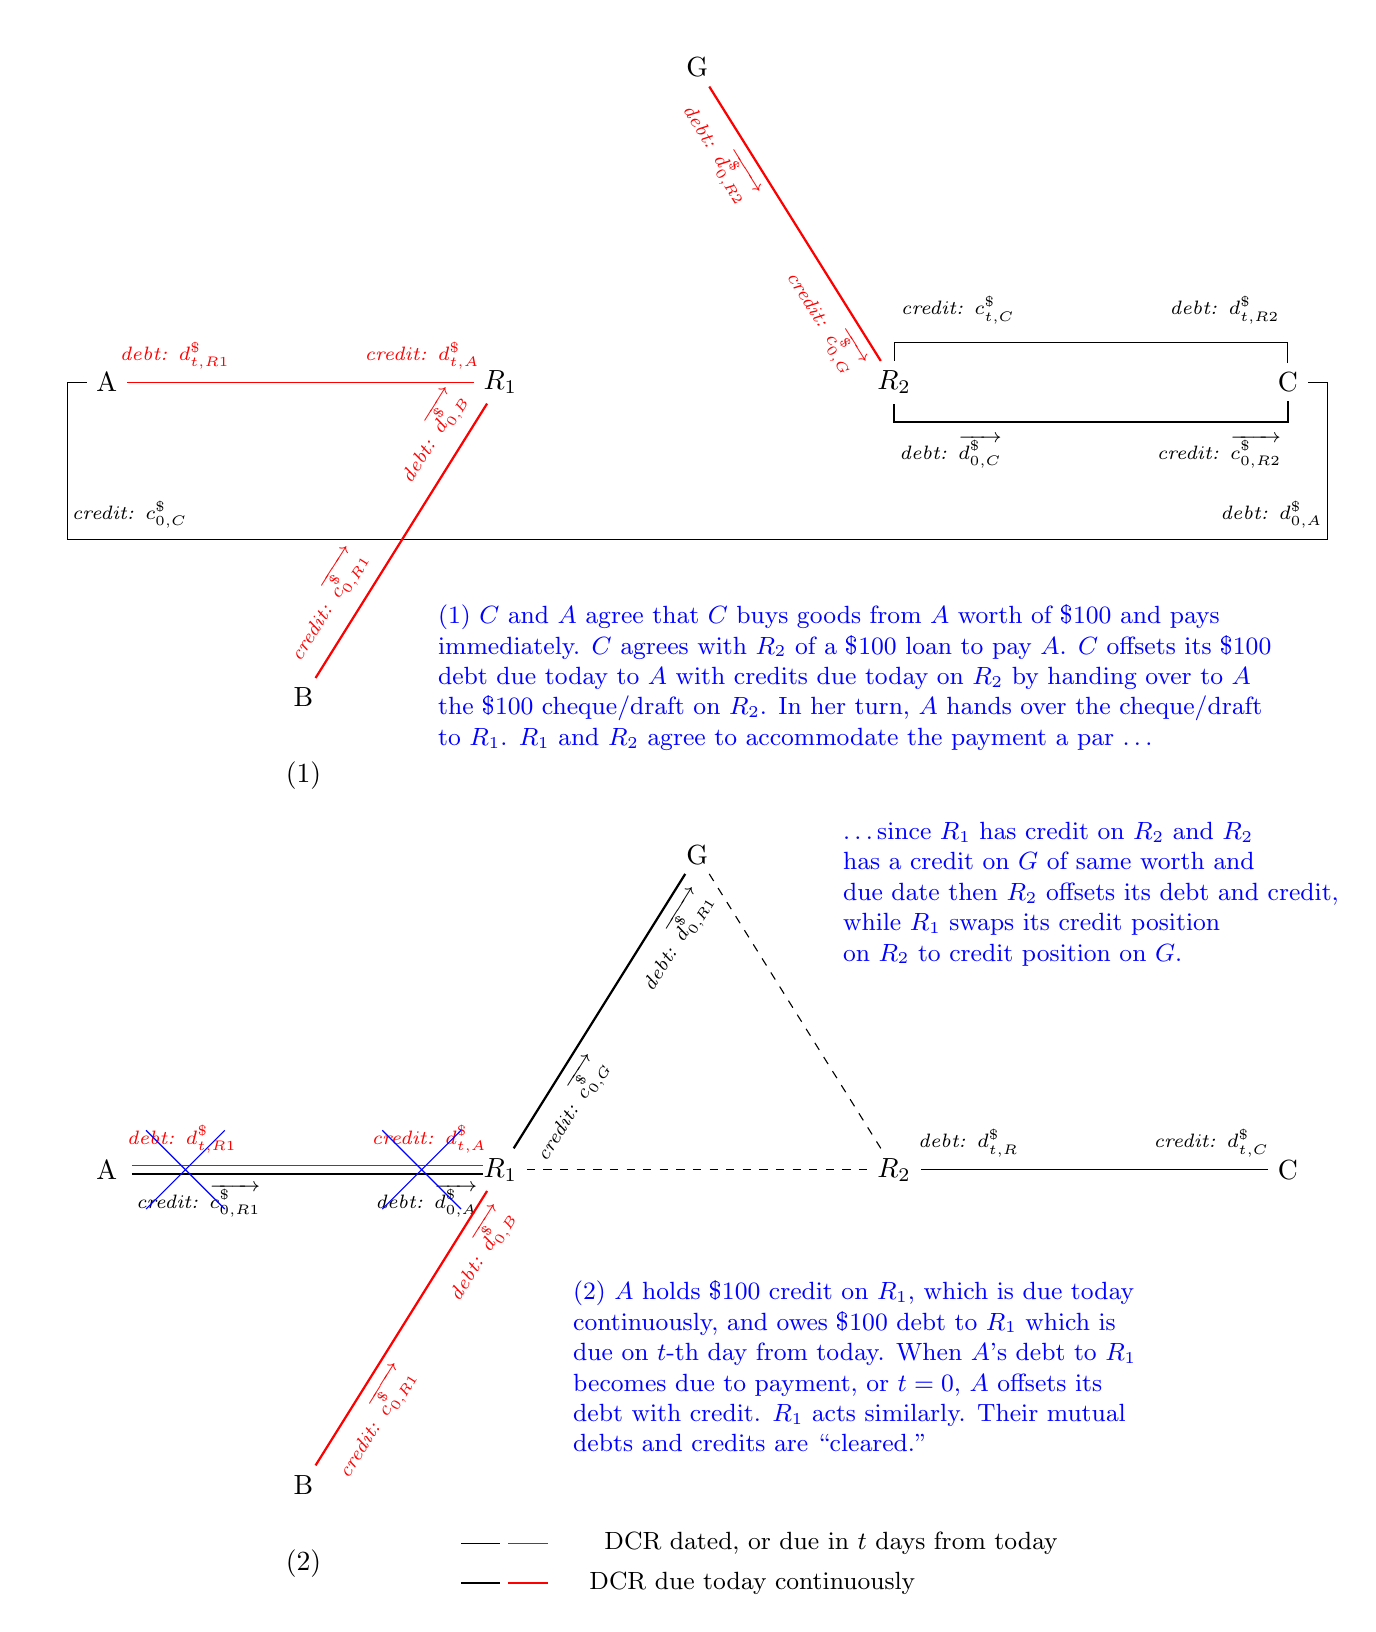
\begin{tikzpicture}
  \draw[help lines,white] (0,0) grid (16,20);
  
  % Middle part of the Figure
  \node         (A)         at (1,15.5) {A};
  \node         (R1)        at (6,15.5) {$R_1$};
  \node         (B)         at (3.5,11.5) {B};
  \node         (R2)        at (11,15.5) {$R_2$};
  \node         (C)         at (16,15.5) {C};
  \node         (G)         at (8.5,19.5) {G};
  \node                     at (3.5,10.5) {(1)};
  %\draw[dashed,blue] (A) to [out=-30,in=-30] node[sloped,below,font=\small]        {$C$ buys goods from $A$} (C);
  \draw[black]   (C.north) |- (14,16) -| (R2.north);
  \draw[black,thick]   (C.south) |- (14,15) -| (R2.south);
  \draw (A.west) -- (.5,15.5) |- (5,13.5) -| (16.5,15.5) -- (C.east);
  \node[align=left] at (1.3,13.8) {\textsuperscript{\textit{credit: }$c^{\$}_{0,C}$}};
  \node[align=left] at (15.8,13.8) {\textsuperscript{\textit{debt: }$d^{\$}_{0,A}$}};
  \node at (13.5,16.4) {\textsuperscript{\textit{credit: }$c^{\$}_{t,C}$ \hspace{.7in} \textit{debt: }$d^{\$}_{t,R2}$}};
  \node at (13.5,14.6) {\textsuperscript{\textit{debt: }$\overrightarrow{d^{\$}_{0,C}}$ \hspace{.7in} \textit{credit: }$\overrightarrow{c^{\$}_{0,R2}}$}}; 
  \draw[red,thick] (G) -- (R2) node[midway,sloped,below]%
        {\textsuperscript{\textit{debt: }$\overrightarrow{d^{\$}_{0,R2}}$ \hspace{.35in} \textit{credit: }$\overrightarrow{c^{\$}_{0,G}}$}};
  \draw[red] (A) -- (R1) node[midway,sloped,above]        {\textsuperscript{\textit{debt: }$d^{\$}_{t,R1}$ \hspace{.6in} \textit{credit: }$d^{\$}_{t,A}$}};
  \draw[red,thick] (B) -- (R1) node[midway,sloped,above]%
        {\textsuperscript{\textit{credit: }$\overrightarrow{c^{\$}_{0,R1}}$ \hspace{.35in} \textit{debt: }$\overrightarrow{d^{\$}_{0,B}}$}};
  \node[blue,align=left,font=\small] at (10.5,11.75) {(1) $C$ and $A$ agree that $C$ buys goods from $A$ worth of \$100 and pays\\immediately. $C$ agrees with $R_2$ of a \$100 loan to pay $A$. $C$ offsets its \$100\\debt due today to $A$ with credits due today on $R_2$ by handing over to $A$\\the \$100 cheque/draft on $R_2$. In her turn, $A$ hands over the cheque/draft\\to $R_1$. $R_1$ and $R_2$ agree to accommodate the payment a par \dots};
  \node[blue,align=left,font=\small] at (13.5,9) {\dots since $R_1$ has credit on $R_2$ and $R_2$\\has a credit on $G$ of same worth and\\due date then $R_2$ offsets its debt and credit,\\while $R_1$ swaps its credit position\\on $R_2$ to credit position on $G$.};
  % Bottom part of the Figure
  \node         (A)         at (1,5.5) {A};
  \node         (R1)        at (6,5.5) {$R_1$};
  \node         (R2)        at (11,5.5) {$R_2$};
  \node         (B)         at (3.5,1.5) {B};  
  \node         (C)         at (16,5.5) {C};
  \node         (G)         at (8.5,9.5) {G};
  \node                     at (3.5,0.5) {(2)};
  %\draw[red] (A) -- (R) node[midway,sloped,above]
  \draw[red] (1.32,5.55) -- (5.78,5.55) node[midway,sloped,above] {\textsuperscript{\textit{debt: }$d^{\$}_{t,R1}$ \hspace{.6in} \textit{credit: }$d^{\$}_{t,A}$}};
  \draw[thick] (1.32,5.45) -- (5.78,5.45)  node[midway,sloped,below]%
        {\textsuperscript{\textit{credit: }$\overrightarrow{c^{\$}_{0,R1}}$ \hspace{.5in} \textit{debt: }$\overrightarrow{d^{\$}_{0,A}}$}};
  \draw[black] (C) -- (R2) node[midway,sloped,above] {\textsuperscript{\textit{debt: }$d^{\$}_{t,R}$ \hspace{.6in} \textit{credit: }$d^{\$}_{t,C}$}};
  \draw[thick] (G) -- (R1) node[midway,sloped,below]%
        {\textsuperscript{\textit{credit: }$\overrightarrow{c^{\$}_{0,G}}$ \hspace{.35in} \textit{debt: }$\overrightarrow{d^{\$}_{0,R1}}$}};
  \draw[red,thick] (B) -- (R1) node[midway,sloped,below]%
        {\textsuperscript{\textit{credit: }$\overrightarrow{c^{\$}_{0,R1}}$ \hspace{.35in} \textit{debt: }$\overrightarrow{d^{\$}_{0,B}}$}};
  %\draw[thick] (R1) -- (R2) node[midway,sloped,above] {\textsuperscript{\textit{credit: }$\overrightarrow{c^{\$}_{0,R2}}$ \hspace{.45in} \textit{debt: }$\overrightarrow{d^{\$}_{0,R1}}$}};
   \draw[blue] (1.5,5)   -- (2.5,6);
   \draw[blue] (1.5,6)   -- (2.5,5);
   \draw[blue] (4.5,5)   -- (5.5,6);
   \draw[blue] (4.5,6)   -- (5.5,5);
   \node[blue,align=left,font=\small] at (10.5,3) {(2) $A$ holds \$100 credit on $R_1$, which is due today\\continuously, and owes \$100 debt to $R_1$ which is\\due on $t$-th day from today. When $A$'s debt to $R_1$\\becomes due to payment, or $t=0$, $A$ offsets its\\debt with credit. $R_1$ acts similarly. Their mutual\\debts and credits are ``cleared."};
   % Labels
  %\draw[black] (5.5,.75) -- (6.5,.75); 
  \draw[dashed] (R1) -- (R2); \draw[dashed] (G) -- (R2); 
  \draw[black] (5.5,.75) -- (6,.75);\draw[red] (6.1,.75) -- (6.6,.75); 
  \node[black,align=left,font=\small] at (10.2,.75) {DCR dated, or due in $t$ days from today};
  %\draw[black,thick] (5.5,0.25) -- (6.5,0.25) 
  \draw[black,thick] (5.5,0.25) -- (6,0.25);\draw[red,thick] (6.1,0.25) -- (6.6,0.25); 
  \node[black,font=\small] at (9.2,0.25) {DCR due today continuously};
\end{tikzpicture}
\caption[Bankers $R_1, R_2$ make loans for trade by $A,B,C$, set-off via $G$]%
{Bankers $R_1, R_2$ make loans for trade by $A,B,C$, set-off via government's bills $G$}
\label{fig:bank_mk_loan4}
\vspace{.1in}
\end{figure}

Concluding the evolutionary aspect of clearing house function, it must be recognized that at the time of writing of \cite{innes1910,innes1913,innes1914} the payments between banks were handled through clearing houses. During the second part of the nineteenth century and until the creation of the System of the Federal Reserve Banks, which is an equivalent to the central bank elsewhere, the major commercial centers such as New York, Boston, Chicago, Philadelphia, New Orleans, St. Louis, Kansas City and others had own Clearing House Association \citep[p.~104]{hubbard1969}. A typical observation of the early twentieth century in this regard was following: ``\dots in the United States \dots we have been for years constantly establishing new clearing houses in places where banks formerly exchanged checks by sending them to one another with their own messengers." \citep[p.~7]{kinley1911} Clearing houses not only allowed banks to economize on the messengers costs, they became an integral part of banks' solvency confirmation that took place on a daily basis.

In each of the center of commerce local banks clubbed together to set up such an association. For example,  in St. Louis of late 1868 there were thirty four local banks that came together to start the Clearing House Association for that city and wider Missouri state. Only about two decades later, in 1885, another commercial center of Missouri in Kansas City saw its banks establishing own \acf{cha}. Hence, at that time ``Kansas City has become \dots practically the clearing house for Kansas, Colorado, New Mexico and Western Missouri the larger portion of whose banks keep their balances, with her banks." \citep[p.~281]{case1888} 

The above description was typical for a regional money center, where banks, being located in a commerical center, clubbed together in the premises of the local \ac{cha} on a daily basis to apply set-off principle to mutual and opposite \acfp{dcr} of the due-today-continuously type. These banks were members of the respective \ac{cha}. Out of town, or country, banks did not have such membership and hence were allowed to participate in the clearing house operations indirectly, which is via a partner bank located in the commercial center and being member of the local \ac{cha}. It was said, as in the quote above, such out-of-town banks kept ``their balances with" banks, which were members of the \ac{cha}. These balances sometimes also called bankers balances or correspondent banking\index{Correspondent banking} relationships. Using the above-mentioned terminology, the out-of-town banks and the banks located in the commercial centers and hence members of the local \ac{cha} maintained \acfp{dcr} of the due-today-continuosly type, where the former had creditor positions, $\overrightarrow{c_0}$, while the latter had debtor positions, $\overrightarrow{d_0}$, against each other. See Figure~\ref{fig:banks_clients_govt2}, p.~\pageref{fig:banks_clients_govt2}, for the general schema of the \acfp{dcr} in a commerical center of the U.S. prior to the Federal Reserve System. The \ac{cha} member banks on daily basis were using two methods of set-off as discussed above: (1) the complete set-off for mutual and opposite \acp{dcr}, and (2) the partial set-off for the remaining \acp{dcr}, where the member bank with a creditor position on other member banks would swap it to the creditor position on the government or a bank in one of large commercial centers.  

\begin{figure}[!ht]
\vspace{.0in}
\captionsetup{width=1\linewidth,labelfont=bf}
  \centering
  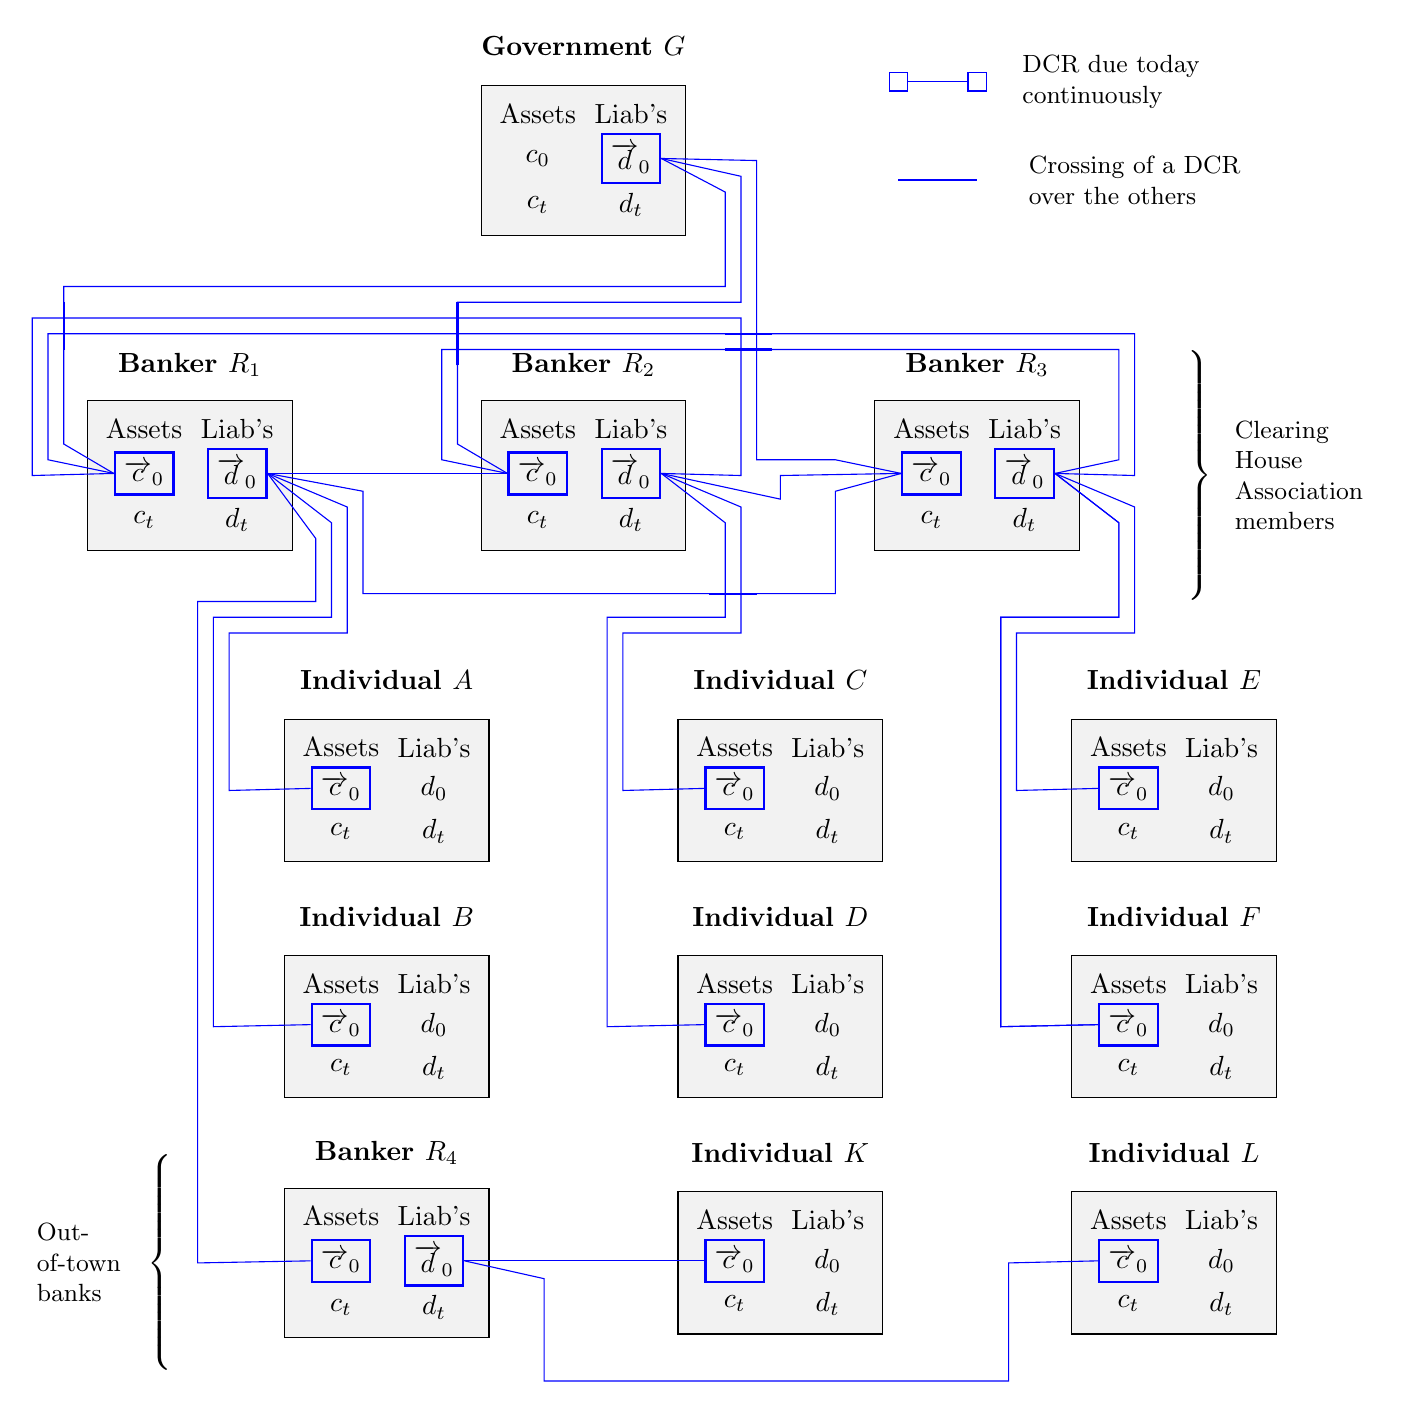
\begin{tikzpicture}
  \draw[help lines,white] (0,0) grid (16,14);  
        % BS of govt (issuer of "lawful money") -----------------------------
        \node [matrix,fill=gray!10,draw=black,thin] (g) at (7,13)
          {
            \node {Assets}; & \node {Liab's}; \\
            \node (G_c0) {$c_0$}; & \node[rectangle,draw=blue,thick] (G_d0)  {$\overrightarrow{d}_0$}; \\
            \node {$c_t$}; & \node {$d_t$}; \\
          };
          \draw (g)++(0,1.45) node[font=\bf]{Government $G$}; 
        % BS of banker R1 ---------------------------------------------------
          \node [matrix,fill=gray!10,draw=black,thin] (b1) at (2,9)
          {
            \node {Assets}; & \node {Liab's}; \\
            \node[rectangle,draw=blue,thick] (R1_c0) {$\overrightarrow{c}_0$}; & \node[rectangle,draw=blue,thick] (R1_d0)  {$\overrightarrow{d}_0$}; \\
            \node {$c_t$}; & \node {$d_t$}; \\
          };
          \draw (b1)++(0,1.4) node[font=\bf]{Banker $R_1$}; 
          \node [matrix,fill=gray!10,draw=black,thin] (b2) at (7,9)
          {
            \node {Assets}; & \node {Liab's}; \\
            \node[rectangle,draw=blue,thick] (R2_c0) {$\overrightarrow{c}_0$}; & \node[rectangle,draw=blue,thick] (R2_d0)  {$\overrightarrow{d}_0$}; \\
            \node {$c_t$}; & \node {$d_t$}; \\
          };
          \draw (b2)++(0,1.4) node[font=\bf]{Banker $R_2$};
          \node [matrix,fill=gray!10,draw=black,thin] (b2) at (12,9)
          {
            \node {Assets}; & \node {Liab's}; \\
            \node[rectangle,draw=blue,thick] (R3_c0) {$\overrightarrow{c}_0$}; & \node[rectangle,draw=blue,thick] (R3_d0)  {$\overrightarrow{d}_0$}; \\
            \node {$c_t$}; & \node {$d_t$}; \\
          };
          \draw (b2)++(0,1.4) node[font=\bf]{Banker $R_3$};
        % BS of private individuals -----------------------------------------
          \node [matrix,fill=gray!10,draw=black,thin] (c1) at (4.5,5)
          {
            \node {Assets}; & \node {Liab's}; \\
            \node[rectangle,draw=blue,thick] (A_c0) {$\overrightarrow{c}_0$}; & \node {$d_0$}; \\
            \node {$c_t$}; & \node {$d_t$}; \\
          };
          \draw (c1)++(0,1.4) node[font=\bf]{Individual $A$};
          \node [matrix,fill=gray!10,draw=black,thin] (h1) at (4.5,2)
          {
            \node {Assets}; & \node {Liab's}; \\
            \node[rectangle,draw=blue,thick] (B_c0) {$\overrightarrow{c}_0$}; & \node {$d_0$}; \\
            \node {$c_t$}; & \node {$d_t$}; \\
          };
          \draw (h1)++(0,1.4) node[font=\bf]{Individual $B$};
          \node [matrix,fill=gray!10,draw=black,thin] (c1) at (9.5,5)
          {
            \node {Assets}; & \node {Liab's}; \\
            \node[rectangle,draw=blue,thick] (C_c0) {$\overrightarrow{c}_0$}; & \node {$d_0$}; \\
            \node {$c_t$}; & \node {$d_t$}; \\
          };
          \draw (c1)++(0,1.4) node[font=\bf]{Individual $C$};
          \node [matrix,fill=gray!10,draw=black,thin] (h1) at (9.5,2)
          {
            \node {Assets}; & \node {Liab's}; \\
            \node[rectangle,draw=blue,thick] (D_c0) {$\overrightarrow{c}_0$}; & \node {$d_0$}; \\
            \node {$c_t$}; & \node {$d_t$}; \\
          };
          \draw (h1)++(0,1.4) node[font=\bf]{Individual $D$};
          \node [matrix,fill=gray!10,draw=black,thin] (h1) at (4.5,-1)
          {
            \node {Assets}; & \node {Liab's}; \\
            \node[rectangle,draw=blue,thick] (R4_c0) {$\overrightarrow{c}_0$}; & \node[rectangle,draw=blue,thick] (R4_d0)  {$\overrightarrow{d}_0$}; \\
            \node {$c_t$}; & \node {$d_t$}; \\
          };
          \draw (h1)++(0,1.4) node[font=\bf]{Banker $R_4$};
          \node [matrix,fill=gray!10,draw=black,thin] (c1) at (14.5,5)
          {
            \node {Assets}; & \node {Liab's}; \\
            \node[rectangle,draw=blue,thick] (E_c0) {$\overrightarrow{c}_0$}; & \node {$d_0$}; \\
            \node {$c_t$}; & \node {$d_t$}; \\
          };
          \draw (c1)++(0,1.4) node[font=\bf]{Individual $E$};
          \node [matrix,fill=gray!10,draw=black,thin] (h1) at (14.5,2)
          {
            \node {Assets}; & \node {Liab's}; \\
            \node[rectangle,draw=blue,thick] (F_c0) {$\overrightarrow{c}_0$}; & \node {$d_0$}; \\
            \node {$c_t$}; & \node {$d_t$}; \\
          };
          \draw (h1)++(0,1.4) node[font=\bf]{Individual $F$};
          \node [matrix,fill=gray!10,draw=black,thin] (h1) at (9.5,-1)
          {
            \node {Assets}; & \node {Liab's}; \\
            \node[rectangle,draw=blue,thick] (K_c0) {$\overrightarrow{c}_0$}; & \node {$d_0$}; \\
            \node {$c_t$}; & \node {$d_t$}; \\
          };
          \draw (h1)++(0,1.4) node[font=\bf]{Individual $K$};
          \node [matrix,fill=gray!10,draw=black,thin] (h1) at (14.5,-1)
          {
            \node {Assets}; & \node {Liab's}; \\
            \node[rectangle,draw=blue,thick] (L_c0) {$\overrightarrow{c}_0$}; & \node {$d_0$}; \\
            \node {$c_t$}; & \node {$d_t$}; \\
          };
          \draw (h1)++(0,1.4) node[font=\bf]{Individual $L$};
          % Debt-credit pairs due today continiously: G vs R1,R2,R3 ------------
          \draw[blue,thin] (R1_c0.west) -- (0.4,9.4) -- (0.4,11.4) -- 
                (8.8,11.4) -- (8.8,12.6) -- (G_d0.east); \draw[blue,thick] (0.4,10.6)--(0.4,11.2);
          \draw[blue,thin] (R2_c0.west) -- (5.4,9.4) -- (5.4,11.2) -- 
                (9,11.2) -- (9,12.8) -- (G_d0.east); \draw[blue,thick] (5.4,10.4)--(5.4,11.2);
          \draw[blue,thin] (R3_c0.west) -- (10.2,9.2) -- (9.2,9.2) -- 
                (9.2,13) --  (G_d0.east); \draw[blue,thick] (5.4,10.4)--(5.4,11.2);
          % Debt-credit pairs due today continiously ---------------------------
          \draw[blue,thin] (R1_d0.east) -- (R2_c0.west);
          \draw[blue,thin] (R1_c0.west) -- (0,9) -- (0,11) -- 
                (9,11) -- (9,9) -- (R2_d0.east);
          \draw[blue,thin] (R1_c0.west) -- (0.2,9.2) -- (0.2,10.8) -- 
                (14,10.8) -- (14,9) -- (R3_d0.east); \draw[blue,thick] (8.8,10.8)--(9.4,10.8);
          \draw[blue,thin] (R2_c0.west) -- (5.2,9.2) -- (5.2,10.6) -- 
                (13.8,10.6) -- (13.8,9.2) -- (R3_d0.east); \draw[blue,thick] (8.8,10.6)--(9.4,10.6);
          \draw[blue,thin] (R2_d0.east) -- (9.5,8.7) -- (9.5,9) -- (R3_c0.west);
          \draw[blue,thin] (R1_d0.east) -- (4.2,8.8) -- (4.2,7.5) -- (10.2,7.5) -- (10.2,8.8) -- (R3_c0.west); \draw[blue,thick] (8.6,7.5)--(9.2,7.5);
          % ... the ones that between a bank and its customers
          \draw[blue,thin] (A_c0.west) -- (2.5,5) -- (2.5,7) -- (4,7) -- (4,8.6) -- (R1_d0.east);
          \draw[blue,thin] (B_c0.west) -- (2.3,2) -- (2.3,7.2) -- (3.8,7.2) -- (3.8,8.4) -- (R1_d0.east);
          \draw[blue,thin] (C_c0.west) -- (7.5,5) -- (7.5,7) -- (9,7) -- (9,8.6) -- (R2_d0.east);
          \draw[blue,thin] (D_c0.west) -- (7.3,2) -- (7.3,7.2) -- (8.8,7.2) -- (8.8,8.4) -- (R2_d0.east);
          \draw[blue,thin] (E_c0.west) -- (12.5,5) -- (12.5,7) -- (14,7) -- (14,8.6) -- (R3_d0.east);
          \draw[blue,thin] (F_c0.west) -- (12.3,2) -- (12.3,7.2) -- (13.8,7.2) -- (13.8,8.4) -- (R3_d0.east);
          \draw[blue,thin] (F_c0.west) -- (12.3,2) -- (12.3,7.2) -- (13.8,7.2) -- (13.8,8.4) -- (R3_d0.east);
          \draw[blue,thin] (R4_c0.west) -- (2.1,-1) -- (2.1,7.4) -- (3.6,7.4) -- (3.6,8.2) -- (R1_d0.east);
          \draw[blue,thin] (R4_d0.east) -- (K_c0.west);
          \draw[blue,thin] (R4_d0.east) -- (6.5,-1.2) -- (6.5,-2.5) -- (12.4,-2.5) -- (12.4,-1) -- (L_c0.west);
          % Labels
          \draw[blue] (11,14) node(a)[draw] {} (12,14) node(b)[draw] {};
          \draw[blue] (a) -- (b);
          \node[black,font=\small,align=left] at (13.7,14) {DCR due today\\continuously};
          \draw[blue,thick] (11,12.75) -- (12,12.75);
          \node[black,font=\small,align=left] at (14,12.75) {Crossing of a DCR\\over the others};
          \node[rectangle,right delimiter=\}] (AA) at (14.5,9) {\tikz{\path (15,14) rectangle (15,11);}}; \node[right=22pt,align=left,font=\small] at (AA.west) {Clearing\\House\\Association\\members};
          \node[rectangle,right delimiter=\{] (BB) at (1.3,-1) {\tikz{\path (1.3,0.8) rectangle (1.3,-1.8);}}; \node[left=5pt,align=left,font=\small] at (BB.east) {Out-\\of-town\\banks};
  \end{tikzpicture}
 \caption[Debt-credit pairs due today continuously: government, banks and individuals]%
  {Debt-credit pairs due today continuously, which are denominated in the single money of account such as dollar (\$), between government ($G$), banks ($R_1, R_2, R_3, R_4$) and their clients ($A,B,C,D,E,F,K,L$).\par\vspace{.05in}Note: (a) the dollar (\$) as money of account is not shown explicitly on this Figure, however, it is assumed to be used to denominate all debts and credits; (b) $t$ is tenor of debts and credits; (c) it is assumed that ``lawful money," which are \acp{dcr} with the government, have been centralized by banks which became $G$'s creditors.}
  \label{fig:banks_clients_govt2}
  \vspace{.1in}
\end{figure}

The principal idea of the \citeauthor{innes1913} writings on the monetary theory was money represent social relationships between debtors and creditors. Over the evoltuion of these relartionships they were represented by a variaty of tangable instruments and verbal descriptions. However, their tangable appearence has been secondary, while their relationsal essense---expressed by debtor and creditor posisitons---has been primary. 

\begin{quote}
When a creditor wants his debt paid, he usually means that he wants to change his debtor; that is to say he wants a credit on a banker, so that he can use it easily, or keep it unused with safety. He, therefore, insists that every private debtor shall, when the debt is due, transfer to him a credit on a reputable banker; and every solvent debtor can satisfy his creditor in this manner.~\citep[p.~406]{innes1913}
\end{quote}

In the quote above, \citeauthor{innes1913} was talking about ``a credit on reputable banker" that would calm down an axiouty of the creditor with respect to his current debtor. Similarly, credit on the government embodied in paper currency, or ``lawful money" could serve that purpose. A bill, a check, or paper currency that might be changing hands, while the just-mentioned creditor acted upon his decision, should be understood as secondary -- it deserves rather to be on the background. Instead, relational positions and their change is what primary.

\subsubsection{Intencity of Money Market}\label{sec:money_mkt}

Given the discussion in the two previous subsections, the notions of solvency and ability to make payment on due terms by different entities of the commercial world---from banks to firms and to private individuals---are key elements of the framework developed by \citeauthor{innes1913}.

Numerous private banks have taken over the responsibility of handling payments of a community or a wider society. On a regular basis and continuously dated debts, $d_t$, are being created. These are created thanks to (a) government levying taxes, (b) banks making loans, and (c) commercial and government purchases of goods and services, including wage labor. These are all, by assumption, denominated in the same money unit of account. On their respective due dates, when $t=0$, these debts, $d_0$, are to be offset with credits due today continuously, $\overrightarrow{c_0}$, on some bank. In their own turn, $\overrightarrow{c_0}$, are being created by government and by banks through making loans or buying goods and services as well as other credits from (i) banks themselves, if done by the cenral bank or by government, or (ii) from banks' customers. 

Hence, there is a dynamic and inter-temporal interplay between creation of \acfp{dcr} of the two basic types: dated and due-today-contnuously. As time goes by, a past dated debt must be offset on its due date with equivalent credit due today within the balance sheet of the debtor, Figure~\ref{fig:temp_structure} on p.~\pageref{fig:temp_structure}. As it was discussed above these offsets might be complete or partial.

Since banks had become dedicated specialists in payments, their solvency is tested on the daily basis as they commit to maintain par value of their demand deposits or, correctly said, their debts due today continuously, $\overrightarrow{d_0}$. They do that on a daily basis by maintaining their balance sheets within key solvency principle, see Equation~\ref{eq:solv_rule_banker}, p.~\pageref{eq:solv_rule_banker}. That is a bank's credits due today continuously it holds on other banks must be at least greater than its debts of same type, which were ordered for payment \textit{today} by the bank's customers plus bank's own due payments on other banks: $\overrightarrow{c_0} \geq \overrightarrow{d_0}$.  

A bank increases own  debts of the due-today-continuously type, $\overrightarrow{d_0}$, in two principle ways: (1)~by making loans or discouning bills as discussed above, Figures~\ref{fig:bank_clearing_house1}-\ref{fig:bank_clearing_house2}, and (2)~by obtaining a credit on another bank, through a \acf{cha} or central bank, which must be counter-balanced with debt to the customer. The second might be done directly and indirectly: the former is via a payment order from the payee's bank, the latter is by own customer, payee, presenting a check on another bank from the payer. 

The principal difference between just-mentioned two way of $\overrightarrow{d_0}$ increase by a bank is in the following. In the first way, the bank increases dated credits, $c_t$, it holds on its customers by equavalent value of $\overrightarrow{d_0}$. In the second way, the bank increases credits due today continuously, $\overrightarrow{c_0}$, on other bank alongside with increase of $\overrightarrow{d_0}$. The first way is under control of the bank, the second one is not as it cannot refuse its customer and must accomodate it.

The way a bank can increases credits due today continuously it holds on other banks through (1) borrowing and (2) selling or discounting of a dated credit, $c_t$, for one of the due-today-continuously type, $\overrightarrow{c_0}$. See Figure~\ref{fig:bank_ds_bill} on p.~\pageref{fig:bank_ds_bill} for the description of the triangular \acfp{dcr} during the discounting of bill -- a bank selling a dated credit would be in the position of individual $B$. The first way increases bank's holding of $\overrightarrow{c_0}$ being counter-balanced by own dated debt, $d_t$, to the lender. It can be secured and unsecured, where the former is general, debenture-type borrowing where creditor relies only on debtor's creditworthioness, observed ability to make due payments. The latter form of borrowing when debtor provides creditor with a collateral, which is a dated credit on third party with proved and high creditworthioness. The second way is effectively a swap of credits accompanied by a charge on net worth as dated debt is being sold with a discount, yielding $\overrightarrow{c_0}<c_t$.

Out of the above-mentioned three ways of shaping the size of $\overrightarrow{c_0}$ for a bank, the last two are under direct control of a bank. Hence, for a bank an acive maintainance of par value for its own $\overrightarrow{d_0}$ requires active money market, where \acfp{dcr} are created, re-used and set-off for the sake of holding $\overrightarrow{c_0}$. Such a market operates \textit{daily} that is in step with banks' daily maintanace of par value on their debts, $\overrightarrow{d_0}$ requires.

\begin{figure}[!ht]
\captionsetup{width=1\linewidth,labelfont=bf}
\vspace{.4in}
\centering
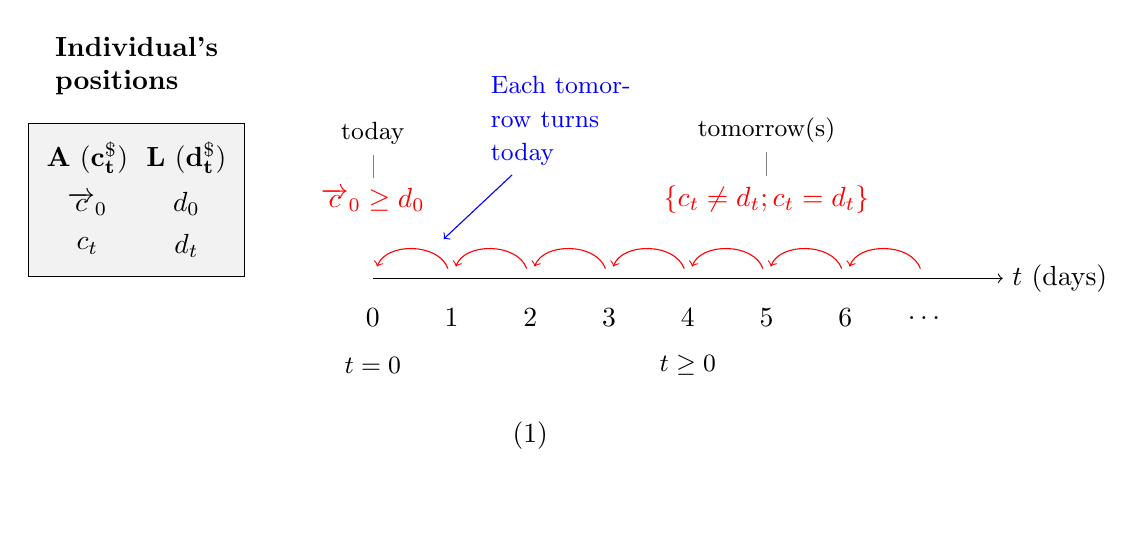
\begin{tikzpicture}[ampersand replacement=\&]
  \draw[help lines,white] (0,0) grid (12,4);
  \node [matrix,fill=gray!10,draw=black,thin] (cb) at (1,2)
  {
    \node {\textbf{A} $\mathbf{(c^{\$}_t)}$}; \& \node {\textbf{L} $\mathbf{(d^{\$}_t)}$}; \\
    \node {$\overrightarrow{c}_0$}; \& \node {$d_0$}; \\
    \node {$c_{\tiny t}$};          \& \node {$d_{\tiny t}$}; \\
  };
  \draw (cb)++(0,1.7) node[font=\bf,align=left]{Individual's\\positions}; 
  \draw[->] (4,1) -- (12,1) node[at end, right] {$t$ (days)};
  \node at (4,-.1) {\small $t=0$};
  \node at (8,-.1) {\small $t \geq 0$}; 
  \node at (6,-1) {(1)}; \node[white] at (6,-2) {}; % <----- BLANK LINE
  \node at (4,.5) (A) {$0$}; \node at (4,1) (a) {}; 
  \node at (5,.5) (B) {$1$}; \node at (5,1) (b) {};
  \node at (6,.5) (C) {$2$}; \node at (6,1) (c) {};
  \node at (7,.5) (D) {$3$}; \node at (7,1) (d) {};
  \node at (8,.5) (E) {$4$}; \node at (8,1) (e) {};
  \node at (9,.5) (F) {$5$}; \node at (9,1) (f) {};
  \node at (10,.5) (G) {$6$}; \node at (10,1) (g) {};
  \node at (11,.5) (H) {$\dots$}; \node at (11,1) (h) {};
  \draw [-{>[sep=.8pt]},red] (b) to [bend right=70] (a);
  \draw [-{>[sep=.8pt]},red] (c) to [bend right=70] (b);
  \draw [-{>[sep=.8pt]},red] (d) to [bend right=70] (c);
  \draw [-{>[sep=.8pt]},red] (e) to [bend right=70] (d);
  \draw [-{>[sep=.8pt]},red] (f) to [bend right=70] (e);
  \draw [-{>[sep=.8pt]},red] (g) to [bend right=70] (f);
  \draw [-{>[sep=.8pt]},red] (h) to [bend right=70] (g);
  \node[red,pin={[pin distance=3mm]above:\small today}] at (4,2) (r_0) 
        {$\overrightarrow{c}_0 \geq d_0$};
  \node[red,pin={[pin distance=3mm]above:\small tomorrow(s)}] at (9,2) (r_T) {$\{ c_t \neq d_t ; c_t=d_t \}$};
  \node [xshift=1cm,yshift=1cm] at (5.5,2) [text width=2cm,blue] (t)
        {\small Each tomorrow turns today};
  \draw [->,blue] (t) -- (4.9,1.5);
\end{tikzpicture}
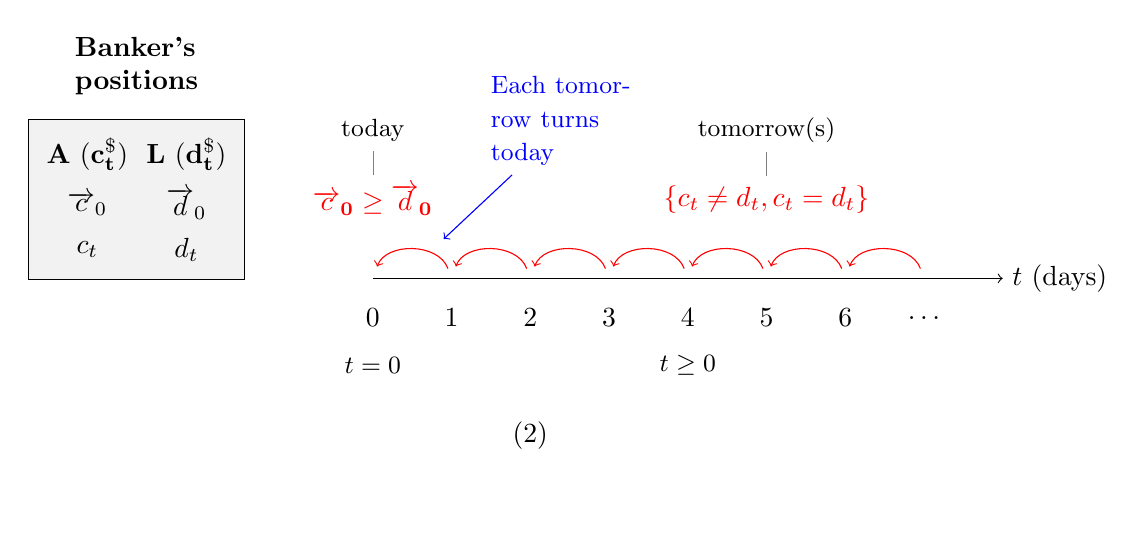
\begin{tikzpicture}[ampersand replacement=\&]
  \draw[help lines,white] (0,0) grid (12,4);
  \node [matrix,fill=gray!10,draw=black,thin] (cb) at (1,2)
  {
    \node {\textbf{A} $\mathbf{(c^{\$}_t)}$}; \& \node {\textbf{L} $\mathbf{(d^{\$}_t)}$}; \\
    \node {$\overrightarrow{c}_0$};      \& \node {$\overrightarrow{d}_0$}; \\
    \node {$c_{\tiny t}$};               \& \node {$d_{\tiny t}$}; \\
  };
  \draw (cb)++(0,1.7) node[font=\bf,align=left]{Banker's\\positions};
  \draw[->] (4,1) -- (12,1) node[at end, right] {$t$ (days)};
  \node at (4,-.1) {\small $t=0$};
  \node at (8,-.1) {\small $t\geq 0$}; 
  \node at (6,-1) {(2)}; \node[white] at (6,-2) {}; % <----- BLANK LINE
  \node at (4,.5) (A) {$0$}; \node at (4,1) (a) {}; 
  \node at (5,.5) (B) {$1$}; \node at (5,1) (b) {};
  \node at (6,.5) (C) {$2$}; \node at (6,1) (c) {};
  \node at (7,.5) (D) {$3$}; \node at (7,1) (d) {};
  \node at (8,.5) (E) {$4$}; \node at (8,1) (e) {};
  \node at (9,.5) (F) {$5$}; \node at (9,1) (f) {};
  \node at (10,.5) (G) {$6$}; \node at (10,1) (g) {};
  \node at (11,.5) (H) {$\dots$}; \node at (11,1) (h) {};
  \draw [-{>[sep=.8pt]},red] (b) to [bend right=70] (a);
  \draw [-{>[sep=.8pt]},red] (c) to [bend right=70] (b);
  \draw [-{>[sep=.8pt]},red] (d) to [bend right=70] (c);
  \draw [-{>[sep=.8pt]},red] (e) to [bend right=70] (d);
  \draw [-{>[sep=.8pt]},red] (f) to [bend right=70] (e);
  \draw [-{>[sep=.8pt]},red] (g) to [bend right=70] (f);
  \draw [-{>[sep=.8pt]},red] (h) to [bend right=70] (g);
  \node[red,pin={[pin distance=3mm]above:\small today}] at (4,2) (r_0) 
        {$\mathbf{\overrightarrow{c}_0 \geq \overrightarrow{d}_0}$};
  \node[red,pin={[pin distance=3mm]above:\small tomorrow(s)}] at (9,2) (r_T) {$\{ c_t \neq d_t , c_t=d_t \}$};
  \node [xshift=1cm,yshift=1cm] at (5.5,2) [text width=2cm,blue] (t)
        {\small Each tomorrow turns today};
  \draw [->,blue] (t) -- (4.9,1.5);
\end{tikzpicture}
\caption[Typical relational positions of individual and banker and their temporal structure]%
{Typical relational positions of individual and banker and their temporal structure\par\vspace{.05in}(1): Typical balance sheet of a merchant, manufacturer, individual and the \textbf{\textit{temporal}} structure of credits (assets) and debts (liabilities) as implied by Mitchell Innes (1913). It implicitly assumes that all credits and debts are denominated in the \underline{single, national} money of account.\par (2): Typical balance sheet of a banker with \textbf{\textit{temporal}} structure of credits (assets) and debts (liabilities). As a specialist the banker maintains a special type of debts ($\overrightarrow{d}_0$), which are due today continuously (or available immediately on a regular basis). The banker's daily solvency relies on the credits of same type ($\overrightarrow{c}_0$), which arise from the transactions with a national central bank or other commercial banks. It implicitly assumes that all credits and debts are denominated in the \underline{single, national} money of account.}
\label{fig:temp_structure}
\vspace{.4in}
\end{figure}

In times of financial panic, when for-profit banks and firms reduce new loans and purchases and instead call for counter parties to pay upon their dated debts early, there is a tendency to prevail when $\overrightarrow{c_0}<\overrightarrow{d_0}$ for banks and $\overrightarrow{c_0}<d_0$ for firms and individuals. This implies that par values could not maintained by banks for their debts $\overrightarrow{d_0}$ and similarly their clients are at riks of non-payments themselves and from their counter parties. In this situations a state actor such a central bank, which is ``almost a government department, must act in reverse and against the wave of shrinking credit creaion:

\begin{quote}
\dots the prospects of the approach of a commercial crisis causes an immediate shrinkage of credit by the banks simultaneously calling in their resources, just at a time when such a shrinkage is likely to be the most disastrous. In countries which have a Central State Bank which is practically a State institution, one might almost say a Government Department, like the Bank of England, the bank is bound to come to the help of the other bankers by creating credit to any extent on good security, irrespective of the state of its gold reserve and the threatened crisis may thus be averted. But here [in the U.S.] there was, until the Aldrich-Vreeland Act came into operation, no institution with the power to create unlimited credit or unlimited currency (the two are practically identical) inspiring the same confidence as gold.~\citep[p.~13-14]{innes1910}
\end{quote}

In situations less stringent than full-blown financial panic, the money market innovations that create credit in reverse to the reduction of it via usual ways proved useful until a more serious and wide-speard panic occured. In early 1900s, some of the regional \acf{cha} innovated this way and created as a by-product a money market for own acknowledgements of debt: 

\begin{quote}
If I am not mistaken the assistance given to the banks of Chicago on the occasion of the failure of an important bank in the city not long ago was organized by the Chicago Clearing House. If the want of a central bank is not more felt it is, I believe, largely due to the beneficent action of the Associations. I am indeed inclined to go so far as to think that all the currency questions that are now being debated by the Monetary Commission might be successfully solved by clothing these Associations with certain powers of issue. \dots In some clearing houses the balances are borrowed and lent either with or without interest. In Chicago the practice of ``trading" the balances, as it is called, has grown to such an extent that it is estimated that bout 75\% of the balances are dealt with in this manner. A bank with a large balance to its credit may trade portions of it to many different banks.~\citep[p.~17-18]{innes1910}
\end{quote}

\subsubsection{Rejection of Medium of Exchange}\label{sec:medium_of_exchange}

\citeauthor{innes1913} was a thinker who in an unwavering fashion adhered to the credit theory of money, which he laid down in his two articles (\citeyear{innes1913,innes1914}). He understood acknowledgements of debt of various forms and embodiments from tally sticks\index{Tally sticks} to gold coins and from government paper currency to checks and drafts on a bank or on a \acf{cha} as primarily an evidence of the existing \acf{dcr}. He recognized their negotiability as new creditors substituted old ones and even used metaphors of motion describing tally sticks and bills travelling ``from hand to hand and from place to
place."\footnote{See p.~396 in \cite{innes1913}.} However, he rejected the notion of ``medium of exchange," which is understood as some commodity money or even paper currency that lubricates exchange. Instead of being facilitated with a medium, exchange itself is an act of debt-credit relationship: ``[a] sale and purchase is the exchange of a commodity for a credit." Hence, ``[t]here is no such thing as a medium of exchange" \citep[p.~168]{innes1914}.

\subsection{\capitalizetitle{Mitchell Innes versus other creditists}}\label{sec:other_creditists}

\begin{figure}[!ht]\centering
\includegraphics[width=1.0\textwidth]{\plotsfolder/econs_lives}
\caption[Major economists writing on the credit theory]%
{Major contributors to the credit theory of money\par \small Red lines indicate years, when major works by the named creditists were published: see \cite{thornton1802}, \cite{colwell1859,colwell1860}, \cite{innes1909,innes1910,innes1913,innes1914,innes1914a,innes1932}
}
\end{figure}

%
% -------------- Stephen Colwell (1800-1871) -----------------------------------+
%
\subsubsection{Stephen Colwell}\index{Colwell, Stephen}

In the United State of mid 19th century, a book titled \textit{The Ways and Means of Payment} was published by Philadelphia-based publisher. It was authored by \citeauthor{colwell1859} (1800-1871), an industrialist from Philadelphia and member of the local elite. See \citep{colwell1859}. 

The author ``had considerable abilities as an economic thinker. \dots  In the 1850s Colwell authored numerous books and articles on topics ranging from the state of manufacturing in Pennsylvania, to the national credit system" \citep[chapter~8, pp.~109-121]{davenport}. 

His biography accounts reveal him as a person, who was an impatient learner of social and economic relations. At the age of thirty six, he started running his father-in-law iron manufacturing business. This took place upon his return from Europe, where he traveled by the insistence of father-in-law to study the state-of-the-arts methods and practices of the local industrialists. He visited England, being attracted to observe firsthand its productive capacities in the midst of Industrial Revolution. In addition, he visited France, Sweden and Belgium \citep[footnote 3, p.~235]{davenport}. He picked up from that learning trip a number of observations that impacted him intellectually. Some accounts mention his dissatisfaction with the observed plight of the working people in the most advanced industrialist lands. He read the works of Adam Smith and critically reviewed his ideas in own writings. His curiosity in the changing world made him great collector of books on the subject of banking and general political economy thought. Upon his death, his personal library consisting of about six thousand titles was handed over to the University of Pennsylvania \citeyearpar[p.~110]{davenport}. He strived to influence the way Americans think of economic matters. In addition to own publications, it appears that he put effort to make the works of German economist Friedrich List published in the United States: the same Philadelphia-based publisher that in 1859 published Colwell's payments book in 1856 published \citeauthor{flist1856}'s major work \textit{National System of Political Economy}. \cite[footnote 12, p.~380]{breton1964} mentioned Colwell as translator of the List's book. Indeed, Colwell favorably viewed the writings of the German economist to such an extent that he wrote an extensive introductory essay to that book, see \citep{colwell1856}. \citeauthor{colwell1859}'s own major work on the subject of political economy was the above-mentioned \textit{The Ways and Means of Payment}, see \citeyearpar{colwell1859}. It became ``his finest treatise" \citep[p.~819]{dorfman2}:    

\begin{quote}
Into its 644 pages Colwell poured a large part of the contents of his vast library on the literature of banking.~\citep[p.~819]{dorfman2}
\end{quote}

A condensed version of the book was put into an article, which was published a year after  \citep{colwell1860}. Indeed, at the time, this book was considered ``the most impressive single work on banking produced in America before 1860" \citep[p.~494]{selgin1989}. 

In this book, \cite{colwell1859,colwell1860} explains the efficiency of the commercial activities as those were utilizing the ``Credit system." For \citeauthor{colwell1859}, the latter epitomized a state of the art system, hence, he referred to it by capitalizing the word credit. He perceived it as being developed from the method of paying with precious meal coins, which was seen as traditional and hence easily and widely recognized. Then, the ``Credit system" detached itself from the ordinary way of payments. His experience with European methods of commerce made him aware of enomous disproportions between payments done through the ``Credit system" and those done with precious metal coins.

\begin{quote}
As more than nine-tenths of all the payments of trade are effected 
without the intervention of gold or silver, it becomes proper to ascertain 
the way in which this large proportion of payments is effected. \dots 
How, then, are the payments chiefly made in the commercial world?~\citep[p.~685]{colwell1860}
\end{quote}

His own research on the payments provided him with the followed brief exposition as an answer:

\begin{quote}
Credits and debts are counterparts -- that is, there being two parties to each debt and 
credit, one is always a debtor and the other always a creditor.~\citep[p.~688]{colwell1860}
The credit system is that by which men set-off\index{Colwell, Stephen!on set-off} the debts wlich others owe them against those which they owe to others.~\citep[p.~8]{colwell1859} 
\end{quote}

In a broad extent, the terminology and its meaning used \citeauthor{colwell1859} was quite similar to \citeauthor{innes1913} as far as technique of payment is concerned.\footnote{For example, compare \citeauthor{colwell1859}'s ``[e]ach individual, in fact, directly or indirectly pays for what he purchases with that which he has to sell"~\citep[p.~190]{colwell1859} with what \citeauthor{innes1913} said: ``[p]urchases \dots are paid for by sales"~\citep[p.~168]{innes1914}.} Thus, Colwell speaks of the mutual claims between transacting counter-parties, which are extinguished through the technique of ``set off" \citep[p.~693]{colwell1860}.\index{Colwell, Stephen!on set-off} However, his description lacks detail of differentiating debts and credits in terms of their tenor or maturity, which is in the forefront of \citeauthor{innes1913}' analysis.

For example, consider the following quote describing payment as complete set-off by \citeauthor{colwell1859} from his book \textit{The Ways and Means of Payment}, which is following by an illustartion of this example in Figure~\ref{fig:set-off-colwell}, p.~\pageref{fig:set-off-colwell}. In this example there two counter parties: the merchant and the manufacturer. The former runs a book of account, where records who owes to whom and the nominal worth of the debts. 

\begin{quote}
The merchant who debits a manufacturer five thousand dollars for raw materials in the course of six months, and gives him credit for finished goods to the amount of seven thousand dollars in the same period, is very willing to unite with his customer in dis charging ten thousand dollars of this debt by balancing the account between them, leaving only two thousand to be paid otherwise than by the balance. The merchant and his customer each receive pay ment of five thousand dollars without money or currency. Each is paid with the debt he owes; the book is the evidence of the debts, and the balancing is the act of payment.~\citep[pp.~8-9]{colwell1859}
\end{quote}

\citeauthor{colwell1859} used verb ``debit" to indicate a change in the debt position of the manufacturer in the merchant's book of account, it meant that manufacturer was buying from the merchant the raw materials worth of \$5,000. Hence, in the merchant's book debiting of the manufacturer account for that worth resulted in an increase of the merchant's credit position on manufacturer by \$5,000. As an mirror image, debt position of manufacturer to the merchant did increase by same size, too. Then, in the quote above giving a credit meant that the merchant was recording a change of the manufacturer's position in the former's book of account. Due to this change, merchant's debt owed to manufacturer increased by \$7,000 and again as an mirror image the manufacturer's credit on the mechant increase by the same size. In other words, merchant was buying from the manufacturer finshed goods worth of \$7,000. Hence, the mentioned counter parties were paying to each other by establishing new dated \acfp{dcr}. These were dated because by mutual agreement they were due in six months. Then, the sides agreed to pay each other by complete set-off for \$5,000 and remaining part of \$2,000 to ``be paid otherwise" or through partial set-off, as a result of which the debtor gives the creditor a swap of the latter's credit position from the current debtor to another debtor, being a banker or the government. 

\begin{figure}[!ht]
\centering
\vspace{.3in}
\captionsetup{width=.8\linewidth,labelfont=bf}
\usetikzlibrary {matrix}
\begin{tikzpicture}
  \draw[help lines,white] (0,0) grid (13,6);
  \node         (A)         at (4,6) {A};
  \node         (B)         at (9,6) {B};
  \node                     at (6.5,5) {(1)};
  \begin{scope}[every node/.style={midway,auto,font=\scriptsize}]
     \draw[black] (A) -- node {$credit^{\$5,000}_{t,B}$ \hspace{0.7in} $debt^{\$5,000}_{t,A}$} (B);
     \draw[red]   (4.25,5.9) -- (8.75,5.9) node[sloped,below]  
                          {$debt^{\$7,000}_{t,B}$ \hspace{.7in} $credit^{\$7,000}_{t,A}$};
  \end{scope}
  \node         (A)         at (4,3) {A};
  \node         (B)         at (9,3) {B};
  \node                     at (6.5,1) {(2)};
  \begin{scope}[every node/.style={midway,auto,font=\scriptsize}]
     \draw[black] (A) -- node {$credit^{\$5,000}_{t,B}$ \hspace{0.7in} $debt^{\$5,000}_{t,A}$} (B);
     \draw[red]   (4.25,2.9) -- (8.75,2.9) node[sloped,below]  
                          {$debt^{\$5,000}_{t,B}$ \hspace{.7in} $credit^{\$5,000}_{t,A}$};
     \draw[blue] (4.5,2.5)   -- (5.5,3.5);
     \draw[blue] (4.5,3.5)   -- (5.5,2.5);
     \draw[blue] (7.75,2.5)  -- (8.75,3.5);
     \draw[blue] (7.75,3.5)  -- (8.75,2.5);
     \draw[red] (A.west) -- (3.5,3) |- (6,2) -| (9.5,3) -- (B.east);
  \end{scope}
  \node[red] at (2.8,2.6) {\textsuperscript{$debt^{\$2,000}_{t,B}$}};
  \node[red] at (10.4,2.6) {\textsuperscript{$credit^{\$2,000}_{t,A}$}};
  \node         (A)         at (4,0) {A};
  \node         (B)         at (9,0) {B};
  \node                     at (6.5,-1) {(3)};
  \begin{scope}[every node/.style={midway,auto,font=\scriptsize}]
     \draw[red]   (A) -- (B) node[sloped,below]  
                          {$debt^{\$2,000}_{t,B}$ \hspace{.7in} $credit^{\$2,000}_{t,A}$};
  \end{scope}
\end{tikzpicture}
\caption[Example of merchant $A$ and manufacturer $B$]%
{Example of merchant $A$ and manufacturer $B$\par\vspace{.05in}(1) They start off with mutual and opposite debt-credit relationships both due in six months or 180 days ($t=180$) but not equal in terms of nominal worth: one is \$5,000 and another is for \$7,000. (2) Set-off is executed for \$5,000. (3) The remaining debt-credit relationship of \$2,000 will ``be paid otherwise."\par Source: narrative from \citep[pp.~8-9]{colwell1859}, illustration by author.}
\label{fig:set-off-colwell}
\vspace{.2in}
\end{figure}

Also, Colwell mentioned what later in the Mitchell Innes writings  was described as sanctity of obligation, albeit in some lighter version: ``[s]o long as a man's own debts are to be regarded as a good currency to pay him with, and he is willing to receive such payment." \citeyearpar[p.~691]{colwell1860}. Then that ``[m]en learned to pay their debts with their credits" \citeyearpar[p.~691]{colwell1860}. Lastly, ``[g]old and silver are seldom lent upon interest; they are never sought for as a medium of payment, because a check upon a bank is preferred" \citeyearpar[p.~694]{colwell1860}. 

Both \citeauthor{colwell1859} and \citeauthor{innes1913} underline the primacy of the money of account concept. It is the language of the commerical activities. The usage of money of account is an established habit and ``a \textit{mental} operation" \citep[p.~3, emphasis added]{colwell1859}. 

What makes \citeauthor{colwell1859} different to \citeauthor{innes1913} is his view that such an efficient system of credit innovated from the previous inefficient circulation of precious metal coins. He conceptualized the ``Credit system" in its conteprory state-of-the-art form well apart from the payments in gold and silver coins, which he regarded as money. He was usually saying throughout his (\citeyear{colwell1859}) book that in the workings of the credit system ``[m]oney was not employed in any large payments"~\citep[p.~190]{colwell1859}.   This thinking is, in fact, similar to the present orthodox presentation of money that today's credit sprang up from the money based upon precious metal. Hence, Colwell stands with one foot in the standard economic theory while another is in the alternative -- the credit theory of money. 

%
% -------------- John R. Commons (1862-1945) ------------------------------+
%
\subsubsection{John R. Commons}\index{Commons, John R.}

In the writings by \citeauthor{commons1951} the credit system is not just a clearing hourse of the commercial activity, it represents what he defined as futurity. And, ``[d]ebts and credits are aspects of futurity." The latter as a concept is about uncertain future upon which, nevertheless, ``the labor and efficiency and bargaining of the future [are] capitalized \textit{beckward} into a present worth"~\citep[p.~103,105]{commons1951}.

For \citeauthor{commons1951} the \acfp{dcr}, which accompany transactions between the members of the community, are representing the workings of the credit system that creates, re-assigns and destroyes money. When ``[m]oney \dots is the center of economic theory, instead of an afterthought \dots the correct picture" emerges~\citep[pp.~643-644,646]{commons1923}.

Concepualization of a transaction in the writings of \citeauthor{commons1951} is quite close to that of \citeauthor{innes1913}. What unites them is recognition that a purchase foremost leads to cretaion of debt for the buyer. \citeauthor{commons1951} talks of this as ``debt of payment," see below, which must be in ``legal money." This should not be taken to be an equivalent of what \citeauthor{innes1913} called ``lawful money" or acknowledgements of debt by the government. In his writings, which were heavily incorporaing the practice of the legal system of the U.S., \citeauthor{commons1951} held a broad definition of the money he deemed legal and those include banks' acknowledgements of debt.

\begin{quote}
[T]wo debts are created by the transaction at a point of time --- a debt
 of payment and a debt of performance. These debts are equivalent to the value willingly
 agreed upon in the transaction. The debt of payment is released by a payment of legal
 money. The debt of performance is released by physical delivery of the materials, services,
 or labor, as measured by other legal units. \citep[p.~241, footnote 7]{commons1936}
 \end{quote}
 
Indeed, the money used for transactions are credits on the banks, while the latter themselves are debts by respective banks. Hence, there is an observance of relationships between debtors and creditors as parties that carry out transactions at present and in the future. 
 
\begin{quote}
The accepted formula of early economists that "goods exchange for goods" fits only a primitive "barter economy." They omitted the bank credit system and the decisions of courts. Shoes are not exchanged for wheat, but both shoes and wheat are today sold for a checking account at a bank, known as a "bank deposit." Even bank "deposit" is a misnomer. It is a bank debt owed by the bank, payable on demand to the "depositor" who, in turn, is not a depositor, but a creditor. By drawing a check on that account he who has sold the shoes in "exchange" for somebody else's check on a bank goes out into other markets and buys with his own check whatever he wishes and can command in exchange. The banking and credit system of the world has destroyed the simplified barter economy of traditional economics. "Goods" do not exchange for "goods"; they are generally sold for a checking account, which is a creditor-debtor relation of contracts enforced by the courts.~\citep[p.~45]{commons1951}
\end{quote}
 
There is also quite close similarity with respect to the typology of \acfp{dcr}. Recall that from the above discussion of \citeauthor{innes1913} this dissertation derived two types of \acp{dcr}: dates and due today continuously. In the quote below, \citeauthor{commons1951} considers, first, debts to which time discounting is being applied and hence their value varies as time goes by. Second, there are debts, in application to which there is no time discounting, and these debts are not dates as they fave no futurity. Rather these debts have status of being available immediately. Demand deposits with bankers have these characteristics.

\begin{quote}
\textit{Some} debts can be used as money, but, for Commons, this supposes that two conditions are satisfied \dots First, debts used as money must be negotiable; their nominative characteristic must be bypassed by the creation of a market that makes them impersonal. The second condition necessary to allow the use of debts as money is that \textit{no time discount} is applied to these debts. This means that their market value does not increase (i.e., time discount decreases) as their maturity comes closer. Thus, debts like commercial papers or bills of exchange cannot be considered as money. For Commons, only one debt satisfies these two properties: the bankers' debts, namely, bank deposits (and more specifically demand deposits). This is so because, unlike securities, demand deposits contain \textit{no futurity}. Bank money is a ``debt past due"; its term is \textit{immediate}, bankers being obligated to supply their debt on demand once they have granted it. Moreover, it is easily transferable from debtors to creditors via the  intermediate role played by bankers. \citep[p.~529, emphasis added]{tymoigne2003}
\end{quote}

Among the scholars of \citeauthor{commons1951} there are two views on how to classify his work. One considered it as leaning towards what is now called as theory of money cuircuit: ``Commons and Keynes had a \textit{circuitist} approach to money"~\citep[p.~528, emphasis added]{tymoigne2003}. Another tended to underscore the futurity concept in which the concept of circulation was relegated: ``\dots we have, not a \textit{circulation} system of money, but a forecast and repetition system of money."~\citep[Commons quoted in][p.~11161, emphasis original]{whalen1993}.

%
% -------------- John M. Keynes (1883-1946) ------------------------------------+
%
\subsubsection{John M. Keynes}\index{Keynes, John M.}

In his early writings, while describing the workings of the money markets in London and other major capitals of the European nations, \citeauthor{keynes1971_1} used the terms ``the balance of immediate indebtedness" and ``claims against [us/them] for immediate payment"~\citep[pp.~13,16]{keynes1971_1}. This category he reserved and applied for the bank balance sheet items of the most sensitive type with respect to payments. In particular, \citeauthor{keynes1971_1} was describing the workings of the London's money market during the gold-exchange standard and the most complicated mechanism guarding ``against a possible drain of specie abroad." In his own words, which came in print as early as in 1913 in the volume \textit{Indian Currency and Finance}:

\begin{quote}
A drain of gold can only come about if foreigners choose to turn into gold claims, which they have against us for immediate payment, and we have no counterbalancing claims against them for equally immediate payment. The drain can only be stopped if we can rapidly bring to bear our counterbalancing claims. When we come to consider how this can best be done, it is to be noticed that the position of a country which is preponderantly a creditor in the international short-loan market is quite different from that of a country which is preponderantly a debtor. In the former case, which is that of Great Britain, it is a question of reducing the amount lent; in the latter case it is a question of increasing the amount borrowed. A machinery which is adapted for action of the first kind may be ill suited for action of the second.~\citep[pp.~12-13]{keynes1971_1}
\end{quote}

\cite[vol.XXV, p.~44]{keynes1980}

\cite{wray1999} criticized \citeauthor{keynes1980}'s \ac{icu} proposal as having two problems. First one is that international monetary system cannot be designed as if trade were `goods against goods`. Second is that its banking analogy is confused. On one hand it is correctly asserts that elimination of convertibility of bancor, money of account in the \ac{icu}, into gold nullifies potential runs on the system. On the other hand, its assertion that balances in bancors might be ``employed to finance" further activity is ``flawed," because by endogenous approach it is loans in bancor create the reserve balances in bancor held by surplus nations \citep[p.~194-198, footnote 16]{wray1999}.\footnote{\cite{wray1999} was published in \cite{harvey1999}.}

%
% -------------- Joseph A. Schumpeter (1883-1946) ------------------------------+
%
\subsubsection{Joseph A. Schumpeter}\index{Schumpeter, Joseph A.}

In \citep{schumpeter2014} there is a dedicated section titled 'How Payment Really Works'.

\citeauthor{wray2009} recognizes that Schumpeter's ``vision of markets was much more orthodox" \citep[p.~810]{wray2009}.

%
% -------------- Hyman P. Minsky (1919-1996) ------------------------------+
%
\subsubsection{Hyman P. Minsky}\index{Minsky, Hyman P.}

\subsection{On the Controversy ``All Money is Credit, but Not All Credit is Money"}
%\subsection{On Critique of \citeauthor{innes1913}' 'All Money is Credit'}\label{sec:critique}

The literature on the \citeauthor{innes1913}'s contribution to monetary economics contains a common thread. It is a controversy around his statement that `` 